%# -*- coding: utf-8-unix -*-
%%==================================================
\tikzset{every picture/.style={line width=0.75pt}} %set default line width to 0.75pt        

\chapter{电磁学}

\begin{mk}{本章符号约定}{}
在电学中,能量,电场,电势能,电动势在高中课本中均用符号$E$来表示,在遇到综合性问题时可能会出现混淆,在未说明的情况下,按照如下符号规则进行区分:

\begin{itemize}
\item 能量使用符号$E_{k0}$来表示,英文下标代表能量类型($k$为动能,$p$为势能等),以数学作为下标区分不同量
\item 电场使用符号$E_a$来表示,以单独的小写英文作为下标
\item 电势能使用$q \Delta \varphi$或者$E_{p0}$来表示(势能只有电势能时)
\item 电动势使用英文E的花体$\ms E$表示\footnote{此处电动势作此约定一方面为了便于区分,另一方面为了跟大学教材的符号约定相同}
\end{itemize}
\end{mk}

\section{杆切割磁场若干二级结论}

此章节中二级结论比较基础且经常用到,在此仅给出简略的证明过程供记忆和查询使用,在此不做过多介绍。

\subsection{不涉及电容}
\begin{center}


\tikzset{every picture/.style={line width=0.75pt}} %set default line width to 0.75pt        

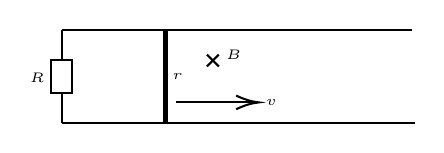
\begin{tikzpicture}[x=0.75pt,y=0.75pt,yscale=-1,xscale=1]
%uncomment if require: \path (0,300); %set diagram left start at 0, and has height of 300

%Straight Lines [id:da0541029549392007] 
\draw    (100,105) -- (269,105) ;
%Straight Lines [id:da4496264717956384] 
\draw    (100,150) -- (270,150) ;
%Shape: Resistor [id:dp8047057543211917] 
\draw   (105,119.71) -- (105,135.55) -- (95,135.55) -- (95,119.71) -- (105,119.71) -- cycle (100,115.25) -- (100,119.71) (100,135.55) -- (100,140) ;
%Straight Lines [id:da051255858179573455] 
\draw    (100,115.25) -- (100,105) ;
%Straight Lines [id:da7781373986650673] 
\draw    (100,150) -- (100,139.75) ;
%Straight Lines [id:da17409470417502937] 
\draw [line width=1.5]    (150,105) -- (150,150) ;
%Straight Lines [id:da5329011887831403] 
\draw    (155,140) -- (193,140) ;
\draw [shift={(195,140)}, rotate = 180] [color={rgb, 255:red, 0; green, 0; blue, 0 }  ][line width=0.75]    (10.93,-3.29) .. controls (6.95,-1.4) and (3.31,-0.3) .. (0,0) .. controls (3.31,0.3) and (6.95,1.4) .. (10.93,3.29)   ;
%Straight Lines [id:da6865175298817716] 
\draw    (170,117) -- (175.7,122.7) ;
%Straight Lines [id:da3716548751829467] 
\draw    (175.7,117) -- (170,122.7) ;


% Text Node
\draw (93,132.15) node [anchor=south east] [inner sep=0.75pt]  [font=\tiny]  {$R$};
% Text Node
\draw (152,127.5) node [anchor=west] [inner sep=0.75pt]  [font=\tiny]  {$r$};
% Text Node
\draw (197,140) node [anchor=west] [inner sep=0.75pt]  [font=\tiny]  {$v$};
% Text Node
\draw (177.7,117) node [anchor=west] [inner sep=0.75pt]  [font=\tiny]  {$B$};


\end{tikzpicture}

\end{center}
如图所示,杆长为$L$,电阻为$r$,两根导轨电阻不计,中间用电阻$R$连接,磁场强度为$B$。记$R_{tot} = R + r$为回路总电阻。
~\\

\noindent \uline{\textbf{通过杆截面电荷量与杆动量变化关系}}

由$F = BIL$两端同乘$\Delta t$可得安培力对杆的动量改变量\footnote{其实就是安培力对杆的冲量,但冲量符号$I$会与电流混淆,故在此用动量改变量描述}为$\Delta p = F \Delta t = BIL \Delta t = BLq$即

\begin{equation}
\boxed{\Delta p = BLq}
\label{e_dhydl}
\end{equation}

\begin{mk}{易错提醒}{}
在使用$q = I \Delta t$时,若电流$I$并非恒定不变,则$I$要取\textbf{关于时间$t$的平均值(不是有效值)}$\bar I$。
~\\

这里需要对\textcolor{magenta}{\textbf{平均值}}跟\textcolor{cyan}{\textbf{有效值}}进行区分:
\begin{itemize}
\item \textcolor{magenta}{\textbf{平均值}}是\textbf{电流}$I$关于时间$t$的平均值$\bar I$
\item \textcolor{cyan}{\textbf{有效值}}是\textbf{电流的平方}$I^2$关于时间$t$的平均值$\overline{I^2}$
\end{itemize}
这里需要注意,一般情况下,$({\bar I})^2 \neq \overline{I^2}$,即\textbf{电流平均值的平方不等于电流平方的平均值}。
~\\

在高中物理中,平均值在力学,电磁学等都具有非常广泛的运用,对于一个平均值,我们必须清楚地知道它\textbf{是什么对什么($x$还是$t$)的平均值}。切记不可将不同的平均值混为一谈。
\end{mk}
~\\

\noindent \uline{\textbf{回路中磁通量变化与回路电荷变化关系}}

由$\ms E = \frac{\Delta \Phi}{\Delta t}$跟$I = \frac{\ms E}{R_{tot}}$可得

$$I = \frac{\Delta \Phi}{R_{tot} \Delta t}$$

两端同乘$\Delta t$,有$q = I \Delta t = \frac{\Delta \Phi}{R_{tot}}$,即

\begin{equation}
\boxed{\Delta q = \frac{\Delta \Phi}{R_{tot}}}
\end{equation}

若回路是线圈之类的存在$n$匝,则

\begin{equation}
\boxed{\Delta q = \frac{n \Delta \Phi}{R_{tot}}}
\end{equation}
~\\

\noindent \uline{\textbf{杆受到外力且达到平衡时外力与杆速度关系}}

\begin{center}


\tikzset{every picture/.style={line width=0.75pt}} %set default line width to 0.75pt        

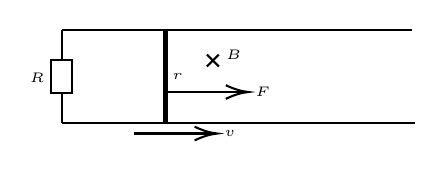
\begin{tikzpicture}[x=0.75pt,y=0.75pt,yscale=-1,xscale=1]
%uncomment if require: \path (0,300); %set diagram left start at 0, and has height of 300

%Straight Lines [id:da0541029549392007] 
\draw    (100,105) -- (269,105) ;
%Straight Lines [id:da4496264717956384] 
\draw    (100,150) -- (270,150) ;
%Shape: Resistor [id:dp8047057543211917] 
\draw   (105,119.71) -- (105,135.55) -- (95,135.55) -- (95,119.71) -- (105,119.71) -- cycle (100,115.25) -- (100,119.71) (100,135.55) -- (100,140) ;
%Straight Lines [id:da051255858179573455] 
\draw    (100,115.25) -- (100,105) ;
%Straight Lines [id:da7781373986650673] 
\draw    (100,150) -- (100,139.75) ;
%Straight Lines [id:da17409470417502937] 
\draw [line width=1.5]    (150,105) -- (150,150) ;
%Straight Lines [id:da5329011887831403] 
\draw    (150,135) -- (188,135) ;
\draw [shift={(190,135)}, rotate = 180] [color={rgb, 255:red, 0; green, 0; blue, 0 }  ][line width=0.75]    (10.93,-3.29) .. controls (6.95,-1.4) and (3.31,-0.3) .. (0,0) .. controls (3.31,0.3) and (6.95,1.4) .. (10.93,3.29)   ;
%Straight Lines [id:da6865175298817716] 
\draw    (170,117) -- (175.7,122.7) ;
%Straight Lines [id:da3716548751829467] 
\draw    (175.7,117) -- (170,122.7) ;

%Straight Lines [id:da49982842161128604] 
\draw    (135,155) -- (173,155) ;
\draw [shift={(175,155)}, rotate = 180] [color={rgb, 255:red, 0; green, 0; blue, 0 }  ][line width=0.75]    (10.93,-3.29) .. controls (6.95,-1.4) and (3.31,-0.3) .. (0,0) .. controls (3.31,0.3) and (6.95,1.4) .. (10.93,3.29)   ;

% Text Node
\draw (93,132.15) node [anchor=south east] [inner sep=0.75pt]  [font=\tiny]  {$R$};
% Text Node
\draw (152,127.5) node [anchor=west] [inner sep=0.75pt]  [font=\tiny]  {$r$};
% Text Node
\draw (192,135) node [anchor=west] [inner sep=0.75pt]  [font=\tiny]  {$F$};
% Text Node
\draw (177.7,117) node [anchor=west] [inner sep=0.75pt]  [font=\tiny]  {$B$};
% Text Node
\draw (177,155) node [anchor=west] [inner sep=0.75pt]  [font=\tiny]  {$v$};


\end{tikzpicture}

\end{center}
如图所示,杆长为$L$,电阻为$r$,两根导轨电阻不计,中间用电阻$R$连接,磁场强度为$B$,杆受到大小为$F$的外力。记$R_{tot} = R + r$为回路总电阻。

由$\ms E = BLv$跟$\ms E = I R_{tot}$得$I = \frac{BLv}{R_{tot}}$,由受力平衡有
$F = BIL = \frac{B^2 L^2 v}{R_{tot}}$,即

\begin{equation}
\boxed{F = \frac{B^2 L^2 v}{R_{tot}}}
\end{equation}

\subsection{涉及电容}

\noindent \uline{\textbf{电容所带电荷与电磁驱动的杆的最大速度}}

\begin{center}


\tikzset{every picture/.style={line width=0.75pt}} %set default line width to 0.75pt        

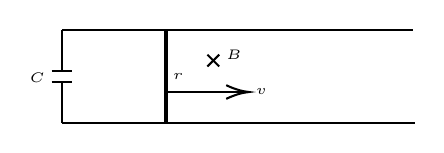
\begin{tikzpicture}[x=0.75pt,y=0.75pt,yscale=-1,xscale=1]
%uncomment if require: \path (0,300); %set diagram left start at 0, and has height of 300

%Straight Lines [id:da0541029549392007] 
\draw    (100,105) -- (269,105) ;
%Straight Lines [id:da4496264717956384] 
\draw    (100,150) -- (270,150) ;
%Straight Lines [id:da051255858179573455] 
\draw    (100,125) -- (100,105) ;
%Straight Lines [id:da7781373986650673] 
\draw    (100,150) -- (100,130) ;
%Straight Lines [id:da17409470417502937] 
\draw [line width=1.5]    (150,105) -- (150,150) ;
%Straight Lines [id:da5329011887831403] 
\draw    (150,135) -- (188,135) ;
\draw [shift={(190,135)}, rotate = 180] [color={rgb, 255:red, 0; green, 0; blue, 0 }  ][line width=0.75]    (10.93,-3.29) .. controls (6.95,-1.4) and (3.31,-0.3) .. (0,0) .. controls (3.31,0.3) and (6.95,1.4) .. (10.93,3.29)   ;
%Straight Lines [id:da6865175298817716] 
\draw    (170,117) -- (175.7,122.7) ;
%Straight Lines [id:da3716548751829467] 
\draw    (175.7,117) -- (170,122.7) ;

%Straight Lines [id:da2785671648689618] 
\draw    (95,130) -- (105,130) ;
%Straight Lines [id:da11367285351862622] 
\draw    (95,125) -- (105,125) ;

% Text Node
\draw (93,132.15) node [anchor=south east] [inner sep=0.75pt]  [font=\tiny]  {$C$};
% Text Node
\draw (152,127.5) node [anchor=west] [inner sep=0.75pt]  [font=\tiny]  {$r$};
% Text Node
\draw (177.7,117) node [anchor=west] [inner sep=0.75pt]  [font=\tiny]  {$B$};
% Text Node
\draw (192,135) node [anchor=west] [inner sep=0.75pt]  [font=\tiny]  {$v$};


\end{tikzpicture}

\end{center}
如图所示,杆长为$L$,电阻为$r$,两根导轨电阻不计,杆初速为$0$,中间用电容$C$连接,初始时带有电荷量$Q_0$,磁场强度为$B$,设某时刻杆的速度为$v$。

对于电容,有$Q = C U$,其中$U$为电容两端电压。当杆\textbf{达到末速}$v_{max}$时,\textbf{杆切割磁场产生的电动势与电容两端电压相同},即$\ms E = U$故

$$\ms E = B l v_{max} = \frac{Q}{C} = U$$

从静止初态到$v_{max}$的末态流经过杆的电荷$\Delta q = Q_0 - Q$。

由前文式\eqref{e_dhydl}可得$m v_{max} = B l \Delta q$,故有


\begin{equation}
\begin{aligned}
B l v_{max} = \frac{Q}{C} \\
\Delta q = Q_0 - Q \\
m v_{max} = B l \Delta q
\end{aligned}
\label{e_drms}
\end{equation}

联立式\eqref{e_drms},解得

\begin{equation}
\boxed{v_{max} = \frac{B L Q_0}{m + C B^2 L^2}}
\end{equation}
~\\

\noindent \uline{\textbf{有电容时受外力杆加速度}}
\begin{center}


\tikzset{every picture/.style={line width=0.75pt}} %set default line width to 0.75pt        

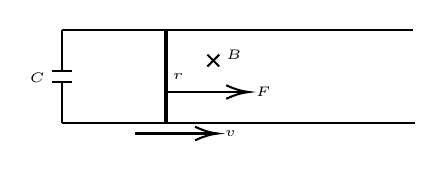
\begin{tikzpicture}[x=0.75pt,y=0.75pt,yscale=-1,xscale=1]
%uncomment if require: \path (0,300); %set diagram left start at 0, and has height of 300

%Straight Lines [id:da0541029549392007] 
\draw    (100,105) -- (269,105) ;
%Straight Lines [id:da4496264717956384] 
\draw    (100,150) -- (270,150) ;
%Straight Lines [id:da051255858179573455] 
\draw    (100,125) -- (100,105) ;
%Straight Lines [id:da7781373986650673] 
\draw    (100,150) -- (100,130) ;
%Straight Lines [id:da17409470417502937] 
\draw [line width=1.5]    (150,105) -- (150,150) ;
%Straight Lines [id:da5329011887831403] 
\draw    (150,135) -- (188,135) ;
\draw [shift={(190,135)}, rotate = 180] [color={rgb, 255:red, 0; green, 0; blue, 0 }  ][line width=0.75]    (10.93,-3.29) .. controls (6.95,-1.4) and (3.31,-0.3) .. (0,0) .. controls (3.31,0.3) and (6.95,1.4) .. (10.93,3.29)   ;
%Straight Lines [id:da6865175298817716] 
\draw    (170,117) -- (175.7,122.7) ;
%Straight Lines [id:da3716548751829467] 
\draw    (175.7,117) -- (170,122.7) ;

%Straight Lines [id:da49982842161128604] 
\draw    (135,155) -- (173,155) ;
\draw [shift={(175,155)}, rotate = 180] [color={rgb, 255:red, 0; green, 0; blue, 0 }  ][line width=0.75]    (10.93,-3.29) .. controls (6.95,-1.4) and (3.31,-0.3) .. (0,0) .. controls (3.31,0.3) and (6.95,1.4) .. (10.93,3.29)   ;
%Straight Lines [id:da2785671648689618] 
\draw    (95,130) -- (105,130) ;
%Straight Lines [id:da11367285351862622] 
\draw    (95,125) -- (105,125) ;

% Text Node
\draw (93,132.15) node [anchor=south east] [inner sep=0.75pt]  [font=\tiny]  {$C$};
% Text Node
\draw (152,127.5) node [anchor=west] [inner sep=0.75pt]  [font=\tiny]  {$r$};
% Text Node
\draw (192,135) node [anchor=west] [inner sep=0.75pt]  [font=\tiny]  {$F$};
% Text Node
\draw (177.7,117) node [anchor=west] [inner sep=0.75pt]  [font=\tiny]  {$B$};
% Text Node
\draw (177,155) node [anchor=west] [inner sep=0.75pt]  [font=\tiny]  {$v$};


\end{tikzpicture}

\end{center}

如图所示,杆长为$L$,电阻为$r$,两根导轨电阻不计,杆受到外力为$F$,中间用电容$C$连接,初始时所带有电荷量为$0$,磁场强度为$B$,设某时刻杆的速度为$v$,加速度为$a$。

取一个某时刻后微小时间$\Delta t$,则有

$$I = \frac{\Delta Q}{\Delta t} = C \frac{\Delta U}{\Delta t} = CBL \frac{\Delta v}{\Delta t} = CBLa$$

由受力分析得

$$F - BIL = ma$$

联立上面两式,解得

\begin{equation}
\boxed{a = \frac{F}{m + C B^2 L^2}}
\end{equation}

\section{“大内偏大,小外偏小”}

\subsection{含义}
高中物理中测电阻或者电源内阻时判断电表内外接时常会教如下口诀“大内偏大,小外偏小”(有时也简化为“内大大,外小小”),其含义如下所示:

\begin{theo}{“大内偏大,小外偏小”}{}

\begin{center}

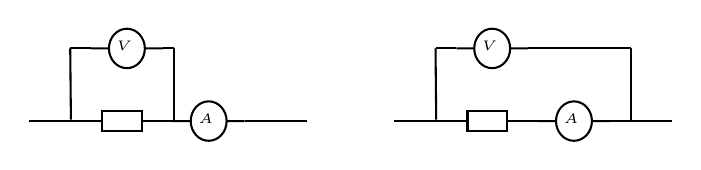
\begin{tikzpicture}[x=0.75pt,y=0.75pt,yscale=-1,xscale=1]
%uncomment if require: \path (0,300); %set diagram left start at 0, and has height of 300

%Shape: Output [id:dp5029694724185756] 
\draw   (238.05,164.5) .. controls (238.05,159.25) and (241.92,155) .. (246.7,155) .. controls (251.48,155) and (255.35,159.25) .. (255.35,164.5) .. controls (255.35,169.75) and (251.48,174) .. (246.7,174) .. controls (241.92,174) and (238.05,169.75) .. (238.05,164.5) -- cycle (229.4,164.5) -- (238.05,164.5) (264,164.5) -- (255.35,164.5) ;
%Straight Lines [id:da5974052849252933] 
\draw    (224.6,129.5) -- (230,129.5) ;
%Shape: Output [id:dp8316238314489566] 
\draw   (198.65,129.5) .. controls (198.65,124.25) and (202.52,120) .. (207.3,120) .. controls (212.08,120) and (215.95,124.25) .. (215.95,129.5) .. controls (215.95,134.75) and (212.08,139) .. (207.3,139) .. controls (202.52,139) and (198.65,134.75) .. (198.65,129.5) -- cycle (190,129.5) -- (198.65,129.5) (224.6,129.5) -- (215.95,129.5) ;
%Straight Lines [id:da8770858852700789] 
\draw    (180,129.5) -- (190,129.5) ;
%Shape: Resistor [id:dp38586331306767896] 
\draw   (195.4,159.5) -- (214.6,159.5) -- (214.6,169.5) -- (195.4,169.5) -- (195.4,159.5) -- cycle (190,164.5) -- (195.4,164.5) (214.6,164.5) -- (220,164.5) ;
%Straight Lines [id:da6656965163696436] 
\draw    (190,164.5) -- (160,164.5) ;
%Straight Lines [id:da878906269405904] 
\draw    (230,164.5) -- (220,164.5) ;
%Straight Lines [id:da9520335954325532] 
\draw    (230,129.5) -- (230,164.5) ;
%Straight Lines [id:da14449988398828695] 
\draw    (294,164.5) -- (264,164.5) ;
%Straight Lines [id:da6761861997187404] 
\draw    (180,129.5) -- (180.33,163.85) ;
%Shape: Output [id:dp49152989281976267] 
\draw   (414.05,164.5) .. controls (414.05,159.25) and (417.92,155) .. (422.7,155) .. controls (427.48,155) and (431.35,159.25) .. (431.35,164.5) .. controls (431.35,169.75) and (427.48,174) .. (422.7,174) .. controls (417.92,174) and (414.05,169.75) .. (414.05,164.5) -- cycle (405.4,164.5) -- (414.05,164.5) (440,164.5) -- (431.35,164.5) ;
%Straight Lines [id:da025922891978220397] 
\draw    (400.6,129.5) -- (450,129.5) ;
%Shape: Output [id:dp10986368699785243] 
\draw   (374.65,129.5) .. controls (374.65,124.25) and (378.52,120) .. (383.3,120) .. controls (388.08,120) and (391.95,124.25) .. (391.95,129.5) .. controls (391.95,134.75) and (388.08,139) .. (383.3,139) .. controls (378.52,139) and (374.65,134.75) .. (374.65,129.5) -- cycle (366,129.5) -- (374.65,129.5) (400.6,129.5) -- (391.95,129.5) ;
%Straight Lines [id:da6881881555017568] 
\draw    (356,129.5) -- (366,129.5) ;
%Shape: Resistor [id:dp538700598242954] 
\draw   (371.4,159.5) -- (390.6,159.5) -- (390.6,169.5) -- (371.4,169.5) -- (371.4,159.5) -- cycle (366,164.5) -- (371.4,164.5) (390.6,164.5) -- (396,164.5) ;
%Straight Lines [id:da9465905183870709] 
\draw    (366,164.5) -- (336,164.5) ;
%Straight Lines [id:da06582730048417962] 
\draw    (406,164.5) -- (396,164.5) ;
%Straight Lines [id:da4945798647049118] 
\draw    (450,129.5) -- (450,164.5) ;
%Straight Lines [id:da23103050393206437] 
\draw    (470,164.5) -- (440,164.5) ;
%Straight Lines [id:da28372038020800505] 
\draw    (356,129.5) -- (356.33,163.85) ;

% Text Node
\draw (240.4,159.5) node [anchor=north west][inner sep=0.75pt]  [font=\tiny] [align=left] {$\displaystyle A$};
% Text Node
\draw (201,124.5) node [anchor=north west][inner sep=0.75pt]  [font=\tiny] [align=left] {$\displaystyle V$};
% Text Node
\draw (416.4,159.5) node [anchor=north west][inner sep=0.75pt]  [font=\tiny] [align=left] {$\displaystyle A$};
% Text Node
\draw (377,124.5) node [anchor=north west][inner sep=0.75pt]  [font=\tiny] [align=left] {$\displaystyle V$};


\end{tikzpicture}

\end{center}

首先我们先定义“内外接”。如图所示,\textbf{电流表在被测元件与电压表回路之外,称为“外接”(左图),电流表在被测元件与电压表回路之内,称为“内接”(右图)。}

记待测元件阻值为$R_x$,电压表内阻为$R_V$,电流表内阻为$R_A$。\textbf{若$R_x > \sqrt{R_v R_A}$(即“大电阻”),则使用“内接”,测量值比准确值偏大。若$R_x < \sqrt{R_v R_A}$(即“小电阻”),则使用“外接”,测量值比准确值偏小。}

\end{theo}

\begin{mk}{易错提醒}{}
这里对于内外接判断需要注意电流表内外接与否\textbf{取决于是否在被测元件与电压表回路之内},对于测量电动势内阻,内外接的概念可能会有偏差,如下:

\begin{center}


\tikzset{every picture/.style={line width=0.75pt}} %set default line width to 0.75pt        

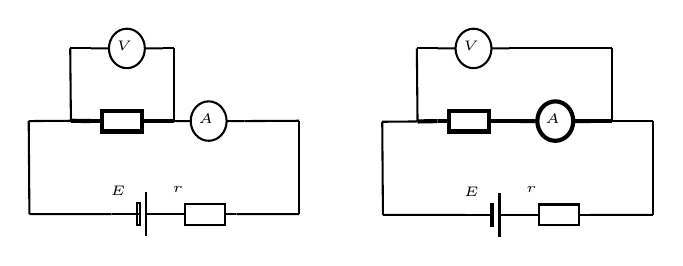
\begin{tikzpicture}[x=0.75pt,y=0.75pt,yscale=-1,xscale=1]
%uncomment if require: \path (0,300); %set diagram left start at 0, and has height of 300

%Shape: Output [id:dp5029694724185756] 
\draw  [line width=0.75]  (237.72,164.5) .. controls (237.72,159.25) and (241.59,155) .. (246.37,155) .. controls (251.14,155) and (255.02,159.25) .. (255.02,164.5) .. controls (255.02,169.75) and (251.14,174) .. (246.37,174) .. controls (241.59,174) and (237.72,169.75) .. (237.72,164.5) -- cycle (229.07,164.5) -- (237.72,164.5) (263.67,164.5) -- (255.02,164.5) ;
%Straight Lines [id:da5974052849252933] 
\draw    (224.27,129.5) -- (229.67,129.5) ;
%Shape: Output [id:dp8316238314489566] 
\draw   (198.32,129.5) .. controls (198.32,124.25) and (202.19,120) .. (206.97,120) .. controls (211.74,120) and (215.62,124.25) .. (215.62,129.5) .. controls (215.62,134.75) and (211.74,139) .. (206.97,139) .. controls (202.19,139) and (198.32,134.75) .. (198.32,129.5) -- cycle (189.67,129.5) -- (198.32,129.5) (224.27,129.5) -- (215.62,129.5) ;
%Straight Lines [id:da8770858852700789] 
\draw    (179.67,129.5) -- (189.67,129.5) ;
%Shape: Resistor [id:dp38586331306767896] 
\draw  [line width=1.5]  (195.07,159.5) -- (214.27,159.5) -- (214.27,169.5) -- (195.07,169.5) -- (195.07,159.5) -- cycle (189.67,164.5) -- (195.07,164.5) (214.27,164.5) -- (219.67,164.5) ;
%Straight Lines [id:da6656965163696436] 
\draw [line width=0.75]    (180,164.35) -- (159.67,164.5) ;
%Straight Lines [id:da878906269405904] 
\draw [line width=1.5]    (229.67,164.5) -- (219.67,164.5) ;
%Straight Lines [id:da9520335954325532] 
\draw    (229.67,129.5) -- (229.67,164.5) ;
%Straight Lines [id:da14449988398828695] 
\draw [line width=0.75]    (290,164.35) -- (263.67,164.5) ;
%Straight Lines [id:da6761861997187404] 
\draw    (179.67,129.5) -- (180,164.35) ;
%Shape: Output [id:dp49152989281976267] 
\draw  [line width=1.5]  (404.72,164.5) .. controls (404.72,159.25) and (408.59,155) .. (413.37,155) .. controls (418.14,155) and (422.02,159.25) .. (422.02,164.5) .. controls (422.02,169.75) and (418.14,174) .. (413.37,174) .. controls (408.59,174) and (404.72,169.75) .. (404.72,164.5) -- cycle (396.07,164.5) -- (404.72,164.5) (430.67,164.5) -- (422.02,164.5) ;
%Straight Lines [id:da025922891978220397] 
\draw    (391.27,129.5) -- (440.67,129.5) ;
%Shape: Output [id:dp10986368699785243] 
\draw   (365.32,129.5) .. controls (365.32,124.25) and (369.19,120) .. (373.97,120) .. controls (378.74,120) and (382.62,124.25) .. (382.62,129.5) .. controls (382.62,134.75) and (378.74,139) .. (373.97,139) .. controls (369.19,139) and (365.32,134.75) .. (365.32,129.5) -- cycle (356.67,129.5) -- (365.32,129.5) (391.27,129.5) -- (382.62,129.5) ;
%Straight Lines [id:da6881881555017568] 
\draw    (346.67,129.5) -- (356.67,129.5) ;
%Shape: Resistor [id:dp538700598242954] 
\draw  [line width=1.5]  (362.07,159.5) -- (381.27,159.5) -- (381.27,169.5) -- (362.07,169.5) -- (362.07,159.5) -- cycle (356.67,164.5) -- (362.07,164.5) (381.27,164.5) -- (386.67,164.5) ;
%Straight Lines [id:da9465905183870709] 
\draw    (347,164.68) -- (330,164.83) ;
%Straight Lines [id:da06582730048417962] 
\draw [line width=1.5]    (396.67,164.5) -- (386.67,164.5) ;
%Straight Lines [id:da4945798647049118] 
\draw    (440.67,129.5) -- (440.67,164.5) ;
%Straight Lines [id:da23103050393206437] 
\draw    (460.67,164.5) -- (440.67,164.5) ;
%Straight Lines [id:da28372038020800505] 
\draw    (346.67,129.5) -- (347,164.68) ;
%Shape: Resistor [id:dp911508638766114] 
\draw  [line width=0.75]  (235.07,204.36) -- (254.27,204.36) -- (254.27,214.36) -- (235.07,214.36) -- (235.07,204.36) -- cycle (229.67,209.36) -- (235.07,209.36) (254.27,209.36) -- (259.67,209.36) ;
%Shape: Battery [id:dp9461258790891913] 
\draw  [line width=0.75]  (199.67,209.36) -- (213.17,209.36) (216.17,198.71) -- (216.17,220) (216.17,209.36) -- (229.67,209.36) (211.97,204.04) -- (213.17,204.04) -- (213.17,214.68) -- (211.97,214.68) -- (211.97,204.04) -- cycle ;
%Straight Lines [id:da810147384196535] 
\draw [line width=0.75]    (160,209.35) -- (199.67,209.36) ;
%Straight Lines [id:da13989104266402697] 
\draw [line width=0.75]    (259.67,209.36) -- (290,209.35) ;
%Straight Lines [id:da8874909650223559] 
\draw [line width=0.75]    (159.67,164.5) -- (160,209.35) ;
%Straight Lines [id:da9588915454156486] 
\draw [line width=0.75]    (290,164.35) -- (290,209.35) ;
%Shape: Resistor [id:dp15732861505999884] 
\draw   (405.4,204.69) -- (424.6,204.69) -- (424.6,214.69) -- (405.4,214.69) -- (405.4,204.69) -- cycle (400,209.69) -- (405.4,209.69) (424.6,209.69) -- (430,209.69) ;
%Shape: Battery [id:dp10154004816535278] 
\draw   (370,209.69) -- (383.5,209.69) (386.5,199.05) -- (386.5,220.33) (386.5,209.69) -- (400,209.69) (382.3,204.37) -- (383.5,204.37) -- (383.5,215.01) -- (382.3,215.01) -- (382.3,204.37) -- cycle ;
%Straight Lines [id:da8110718718276668] 
\draw    (330.33,209.68) -- (370,209.69) ;
%Straight Lines [id:da29331953697412794] 
\draw    (430,209.69) -- (460.33,209.68) ;
%Straight Lines [id:da7332321698809419] 
\draw    (330,164.83) -- (330.33,209.68) ;
%Straight Lines [id:da5024685189170686] 
\draw    (460.33,164.68) -- (460.33,209.68) ;
%Straight Lines [id:da1925989380681068] 
\draw [line width=1.5]    (189.67,164.5) -- (180,164.35) ;
%Straight Lines [id:da2210115814506841] 
\draw [line width=1.5]    (356.67,164.5) -- (347,164.68) ;
%Straight Lines [id:da07809283398760769] 
\draw [line width=1.5]    (440.67,164.5) -- (430.67,164.5) ;

% Text Node
\draw (240.07,159.5) node [anchor=north west][inner sep=0.75pt]  [font=\tiny] [align=left] {$\displaystyle A$};
% Text Node
\draw (200.67,124.5) node [anchor=north west][inner sep=0.75pt]  [font=\tiny] [align=left] {$\displaystyle V$};
% Text Node
\draw (407.07,159.5) node [anchor=north west][inner sep=0.75pt]  [font=\tiny] [align=left] {$\displaystyle A$};
% Text Node
\draw (367.67,124.5) node [anchor=north west][inner sep=0.75pt]  [font=\tiny] [align=left] {$\displaystyle V$};
% Text Node
\draw (201.67,192.86) node [anchor=north west][inner sep=0.75pt]   [align=left] {$ $};
% Text Node
\draw (197.67,194.36) node [anchor=north west][inner sep=0.75pt]  [font=\tiny] [align=left] {$\displaystyle \ms E$};
% Text Node
\draw (227.67,194.36) node [anchor=north west][inner sep=0.75pt]  [font=\tiny] [align=left] {$\displaystyle r$};
% Text Node
\draw (372,193.19) node [anchor=north west][inner sep=0.75pt]   [align=left] {$ $};
% Text Node
\draw (368,194.69) node [anchor=north west][inner sep=0.75pt]  [font=\tiny] [align=left] {$\displaystyle \ms E$};
% Text Node
\draw (398,194.69) node [anchor=north west][inner sep=0.75pt]  [font=\tiny] [align=left] {$\displaystyle r$};


\end{tikzpicture}

\end{center}

由于我们这里要测量的值为电动势内阻,故在被测元件与电压表回路之外的电路为图中粗线所示,因此\textbf{在测量电动势时,左图为“内接”,右图为“外接”。}
\end{mk}

\subsection{证明}
“大内偏大,小外偏小”大多资料书并不会对此做解释和证明,只是填鸭子式蒙混过关。下面我们给出此定理的详细证明。
~\\

\noindent \uline{\textbf{“内接偏大、外接偏小”证明}}

对于“内接测量电阻偏大,外接测量电阻偏小”的证明,一个比较方便的方法是用等效电阻判断。我们可以认为电表就是一个可以显示其电压或电流的电阻,因此对于内接法和外接法,我们可以分别画出如下示意图(左图为外接法,右图为内接法)

\begin{center}

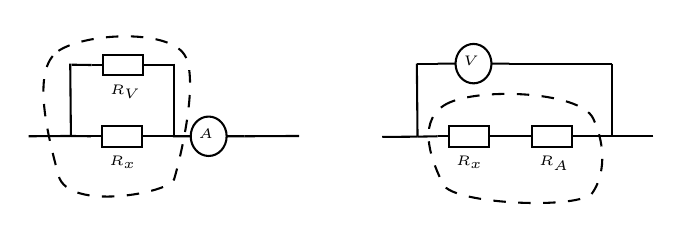
\begin{tikzpicture}[x=0.75pt,y=0.75pt,yscale=-1,xscale=1]
%uncomment if require: \path (0,300); %set diagram left start at 0, and has height of 300

%Shape: Output [id:dp5029694724185756] 
\draw  [line width=0.75]  (237.72,164.5) .. controls (237.72,159.25) and (241.59,155) .. (246.37,155) .. controls (251.14,155) and (255.02,159.25) .. (255.02,164.5) .. controls (255.02,169.75) and (251.14,174) .. (246.37,174) .. controls (241.59,174) and (237.72,169.75) .. (237.72,164.5) -- cycle (229.07,164.5) -- (237.72,164.5) (263.67,164.5) -- (255.02,164.5) ;
%Shape: Resistor [id:dp38586331306767896] 
\draw  [line width=0.75]  (195.07,159.5) -- (214.27,159.5) -- (214.27,169.5) -- (195.07,169.5) -- (195.07,159.5) -- cycle (189.67,164.5) -- (195.07,164.5) (214.27,164.5) -- (219.67,164.5) ;
%Straight Lines [id:da6656965163696436] 
\draw [line width=0.75]    (180,164.35) -- (159.67,164.5) ;
%Straight Lines [id:da878906269405904] 
\draw [line width=0.75]    (229.67,164.5) -- (219.67,164.5) ;
%Straight Lines [id:da9520335954325532] 
\draw    (229.67,129.5) -- (229.67,164.5) ;
%Straight Lines [id:da14449988398828695] 
\draw [line width=0.75]    (290,164.35) -- (263.67,164.5) ;
%Straight Lines [id:da6761861997187404] 
\draw    (179.67,129.5) -- (180,164.35) ;
%Straight Lines [id:da025922891978220397] 
\draw    (391.27,129.5) -- (440.67,129.5) ;
%Shape: Output [id:dp10986368699785243] 
\draw   (365.32,129.5) .. controls (365.32,124.25) and (369.19,120) .. (373.97,120) .. controls (378.74,120) and (382.62,124.25) .. (382.62,129.5) .. controls (382.62,134.75) and (378.74,139) .. (373.97,139) .. controls (369.19,139) and (365.32,134.75) .. (365.32,129.5) -- cycle (356.67,129.5) -- (365.32,129.5) (391.27,129.5) -- (382.62,129.5) ;
%Straight Lines [id:da6881881555017568] 
\draw    (346.67,129.5) -- (356.67,129.5) ;
%Shape: Resistor [id:dp538700598242954] 
\draw  [line width=0.75]  (362.07,159.5) -- (381.27,159.5) -- (381.27,169.5) -- (362.07,169.5) -- (362.07,159.5) -- cycle (356.67,164.5) -- (362.07,164.5) (381.27,164.5) -- (386.67,164.5) ;
%Straight Lines [id:da9465905183870709] 
\draw    (347,164.68) -- (330,164.83) ;
%Straight Lines [id:da06582730048417962] 
\draw [line width=0.75]    (396.67,164.5) -- (386.67,164.5) ;
%Straight Lines [id:da4945798647049118] 
\draw    (440.67,129.5) -- (440.67,164.5) ;
%Straight Lines [id:da23103050393206437] 
\draw    (460.67,164.5) -- (440.67,164.5) ;
%Straight Lines [id:da28372038020800505] 
\draw    (346.67,129.5) -- (347,164.68) ;
%Straight Lines [id:da1925989380681068] 
\draw [line width=0.75]    (189.67,164.5) -- (180,164.35) ;
%Straight Lines [id:da2210115814506841] 
\draw [line width=0.75]    (356.67,164.5) -- (347,164.68) ;
%Straight Lines [id:da07809283398760769] 
\draw [line width=0.75]    (440.67,164.5) -- (426.67,164.5) ;
%Shape: Resistor [id:dp23145512054728878] 
\draw  [line width=0.75]  (195.4,125.17) -- (214.6,125.17) -- (214.6,135.17) -- (195.4,135.17) -- (195.4,125.17) -- cycle (190,130.17) -- (195.4,130.17) (214.6,130.17) -- (220,130.17) ;
%Straight Lines [id:da5456148753878571] 
\draw [line width=0.75]    (230,130.17) -- (220,130.17) ;
%Straight Lines [id:da4430188841728988] 
\draw [line width=0.75]    (190,130.17) -- (180.33,130.02) ;
%Shape: Resistor [id:dp7255506677378272] 
\draw  [line width=0.75]  (402.07,159.5) -- (421.27,159.5) -- (421.27,169.5) -- (402.07,169.5) -- (402.07,159.5) -- cycle (396.67,164.5) -- (402.07,164.5) (421.27,164.5) -- (426.67,164.5) ;
%Shape: Polygon Curved [id:ds8586201944695224] 
\draw  [dash pattern={on 4.5pt off 4.5pt}] (174,123.35) .. controls (187.67,114.35) and (229,112.68) .. (235.33,126.35) .. controls (241.67,140.02) and (231.67,179.02) .. (229.67,185.35) .. controls (227.67,191.68) and (178.67,201.02) .. (174,183.35) .. controls (169.33,165.68) and (160.33,132.35) .. (174,123.35) -- cycle ;
%Shape: Polygon Curved [id:ds12750654307195575] 
\draw  [dash pattern={on 4.5pt off 4.5pt}] (359.67,149.68) .. controls (373.33,140.68) and (425.33,142.35) .. (431.67,156.02) .. controls (438,169.68) and (437,183.35) .. (431.33,191.68) .. controls (425.67,200.02) and (364,197.35) .. (359.33,187.68) .. controls (354.67,178.02) and (346,158.68) .. (359.67,149.68) -- cycle ;

% Text Node
\draw (240.07,159.5) node [anchor=north west][inner sep=0.75pt]  [font=\tiny] [align=left] {$\displaystyle A$};
% Text Node
\draw (367.67,124.5) node [anchor=north west][inner sep=0.75pt]  [font=\tiny] [align=left] {$\displaystyle V$};
% Text Node
\draw (197.07,172.5) node [anchor=north west][inner sep=0.75pt]  [font=\tiny] [align=left] {$\displaystyle R_{x}$};
% Text Node
\draw (197.4,138.17) node [anchor=north west][inner sep=0.75pt]  [font=\tiny] [align=left] {$\displaystyle R_{V}$};
% Text Node
\draw (364.07,172.5) node [anchor=north west][inner sep=0.75pt]  [font=\tiny] [align=left] {$\displaystyle R_{x}$};
% Text Node
\draw (404.07,172.5) node [anchor=north west][inner sep=0.75pt]  [font=\tiny] [align=left] {$\displaystyle R_{A}$};


\end{tikzpicture}

\end{center}

上图中,我们可以将在内测的电阻等效为一个电阻(如图中虚线所示),该电阻为实际上测量得出的电阻,即电路实际上测量的是虚线内等效的电阻阻值。因此,设待测电阻阻值为$R_x$,电压表内阻$R_V$,电流表内阻$R_A$,内接法测量的阻值为$R_{in}$,外接法测量的阻值为$R_{out}$,则

\begin{equation}
\boxed{R_{out} = \frac{R_V R_x}{R_V + R_x} < R_x ,\quad R_{in} = R_A + R_x > R_x}
\end{equation}

即“内接偏大、外接偏小”,QED。
~\\

\noindent \uline{\textbf{“大电阻选内接、小电阻选外接”证明}}

由前文可知内接时内阻测量偏大、外接内阻测量偏小。记$\Delta R_{in}$为内接时测量值与准确值偏差。$\Delta R_{out}$为外接时测量值与准确值偏差。因此

$$\Delta R_{in} = R_A + R_x - R_x = R_A ,\quad \Delta R_{out} = R_x - \frac{R_x R_V}{R_x + R_V} = \frac{R_x^2}{R_x + R_V}$$

由此我们可以看出,当$R_x$越大时,易证明$\Delta R_{out}$单调递增,因此当$\Delta R_{out} > \Delta R_{in}$时,即电阻足够大时,内接偏差小,选择内接;当$\Delta R_{out} < \Delta R_{in}$时,即电阻足够小时,外接偏差小,选择外接,即“大电阻选内接、小电阻选外接”,QED。
~\\

\noindent \uline{\textbf{大电阻、小电阻判断标准}}

现在我们计算大小电阻的判断标准。易知当$\Delta R_{in} = \Delta R_{out}$时的$R_x$为大小电阻分界线,故

$$R_A = \frac{R_x^2}{R_x + R_V}$$

$$\frac{R_x^2}{R_V} = R_A + R_x \frac{R_A}{R_V}$$

这里有一个近似,一般而言电流表内阻$R_A$远小于电压表内阻$R_V$,故$\frac{R_A}{R_V}$约等于$0$,这一项舍掉,故

\begin{equation}
\boxed{R_x = \sqrt{R_A R_V}}
\end{equation}

因此,若$R_x > \sqrt{R_A R_V}$,我们认为其为大电阻,选内接;若$R_x < \sqrt{R_A R_V}$,我们认为其为小电阻,选外接;若$R_x = \sqrt{R_A R_V}$,内外接均可(虽然一般不会出现这种情况)。

\begin{mk}{易错提醒}{}
“大内偏大,小外偏小”一般用于在两个电表均未知其准确内阻时使用,或在两个电表均已知其准确内阻时使用\footnote{此时内外接其实均可,内外接都可以给分,但习题答案一般仍旧遵循“大内偏大,小外偏小”的原则给出解析}。\textbf{若有一个电表准确内阻已知另一个未知,则可不遵循“大内偏大、小外偏小”的原则选择内外接,而是将精确的电表放“外侧”,在之后的计算中通过已知的准确内阻消除电表内阻的影响。}对于不同的习题,应灵活运用。
\end{mk}

又有“大内偏大,小外偏小”定理几乎在任意一道电学实验题均可运用,且老师讲题时以及答案一般会运用此方法给出详解。故在此不再给出例题。

\section{电源输出功率性质}
\label{s_wdlzdgl}

现有一个电动势为$\ms E$、内阻为$r$的电源,跟一个电阻为$R$的可变电阻串联,现推导电源输出功率功率与电阻阻值关系。

\begin{subequations}
\begin{align*}
I &= \frac{\ms E}{r + R} \\
P &= I^2 R = \frac{\ms E^2 R}{(r + R)^2}
\end{align*}
\end{subequations}

上面$P = \frac{\ms E^2 R}{(r + R)^2}$中$P$关于$R$的函数图像如下图所示(取$\ms E = 1$、$r = 1$)

\begin{figure}[htbp]
\centering
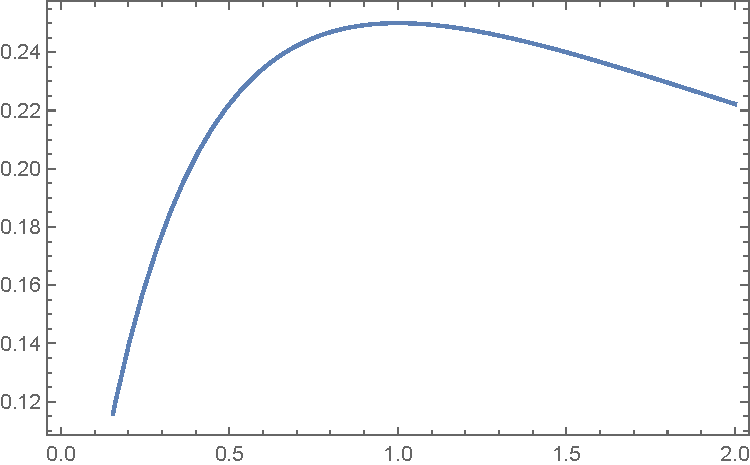
\includegraphics[width=0.5\textwidth]{pic_eled/zdgl_p1.pdf}
\end{figure}

可见存在$R$,使得$P$取得最大值。对$P = \frac{\ms E^2 R}{(r + R)^2}$求导,得

$$P^{\prime}(R) = \frac{\ms E^2}{(r+R)^2}-\frac{2 R \ms E^2}{(r+R)^3} = \frac{\ms E^2 (r-R)}{(r+R)^3}$$

可见,当$R=r$时,$P^{\prime} = 0$,此时$P$最大。由图可知,$R$越接近$r$,电源输出功率$P$越大。并且,若$P$已知,我们可以从$P$中反解出功率相同的两个$R$的关系,化简得到

$$P R^2 + (2 r P - \ms E^2)R + P r^2 = 0$$

由韦达(Vieta)定理:$R$的两根满足$R_1 R_2 = r^2$,即$r = \sqrt{R_1 R_2}$,故

\begin{theo}{电源输出功率性质}{}
当外电路总电阻$R$等于电源内阻$r$时,电源输出功率最大;

外电路总电阻$R$越接近电源内阻$r$,电源输出功率越大;

若两个不同的外电路总电阻对应同一电源输出功率,则这两个外电路总电阻满足$r = \sqrt{R_1 R_2}$。
\end{theo}

运用此定理,结合后文\secref{s_dxy},我们可以很快地求出变化电阻的功率最大问题。

\begin{ep}{练习题(有删减)}{}
\begin{center}
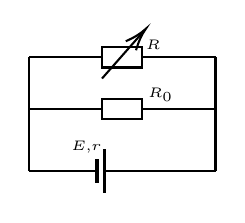
\begin{tikzpicture}[x=0.75pt,y=0.75pt,yscale=-1,xscale=1]
%uncomment if require: \path (0,300); %set diagram left start at 0, and has height of 300

%Shape: Battery [id:dp2916012360245832] 
\draw   (262.5,144) -- (276,144) (279,133.36) -- (279,154.64) (279,144) -- (292.5,144) (274.8,138.68) -- (276,138.68) -- (276,149.32) -- (274.8,149.32) -- (274.8,138.68) -- cycle ;
%Straight Lines [id:da2734255254924993] 
\draw    (242.5,89) -- (242.5,144) ;
%Straight Lines [id:da8342089479991157] 
\draw    (332.5,89) -- (332.5,144) ;
%Straight Lines [id:da4571525926989708] 
\draw    (242.5,144) -- (262.5,144) ;
%Straight Lines [id:da08274074907134321] 
\draw    (292.5,144) -- (332.5,144) ;
%Shape: Resistor [id:dp8558892883342235] 
\draw   (277.9,109) -- (297.1,109) -- (297.1,119) -- (277.9,119) -- (277.9,109) -- cycle (272.5,114) -- (277.9,114) (297.1,114) -- (302.5,114) ;
%Straight Lines [id:da7537185022486395] 
\draw    (272.5,114) -- (242.5,114) ;
%Straight Lines [id:da8797643160506492] 
\draw    (332.5,114) -- (302.5,114) ;
%Shape: Resistor [id:dp5429151855494494] 
\draw   (277.9,84) -- (297.1,84) -- (297.1,94) -- (277.9,94) -- (277.9,84) -- cycle (272.5,89) -- (277.9,89) (297.1,89) -- (302.5,89) ;
%Straight Lines [id:da9804503401878168] 
\draw    (272.5,89) -- (242.5,89) ;
%Straight Lines [id:da5427185273385342] 
\draw    (332.5,89) -- (302.5,89) ;
%Straight Lines [id:da37813397906193025] 
\draw    (277.81,99.32) -- (297.64,76.82) ;
\draw [shift={(298.96,75.32)}, rotate = 131.4] [color={rgb, 255:red, 0; green, 0; blue, 0 }  ][line width=0.75]    (10.93,-3.29) .. controls (6.95,-1.4) and (3.31,-0.3) .. (0,0) .. controls (3.31,0.3) and (6.95,1.4) .. (10.93,3.29)   ;

% Text Node
\draw (264.5,127.05) node [anchor=north west][inner sep=0.75pt]   [align=left] {$ $};
% Text Node
\draw (261.5,128) node [anchor=north west][inner sep=0.75pt]  [font=\tiny] [align=left] {$\displaystyle E$,$\displaystyle r$};
% Text Node
\draw (298.5,102.55) node [anchor=north west][inner sep=0.75pt]  [font=\tiny] [align=left] {$\displaystyle R_{0}$};
% Text Node
\draw (297.5,79.05) node [anchor=north west][inner sep=0.75pt]  [font=\tiny] [align=left] {$\displaystyle R$};


\end{tikzpicture}
\end{center}
如图所示,电源电动势$E=2V$,内阻$r=1\Omega$,电阻$R_0=2\Omega$,可变电阻$R$可从$0\Omega$到$10\Omega$内任意调节。问当可变电阻$R$等于多少时,$R$上消耗功率最大,并求出最大消耗功率。
~\\

\begin{center}
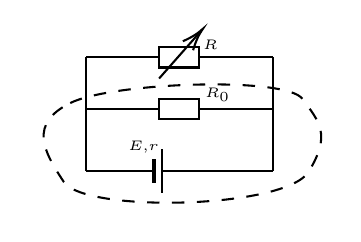
\begin{tikzpicture}[x=0.75pt,y=0.75pt,yscale=-1,xscale=1]
%uncomment if require: \path (0,300); %set diagram left start at 0, and has height of 300

%Shape: Battery [id:dp2916012360245832] 
\draw   (262.5,144) -- (276,144) (279,133.36) -- (279,154.64) (279,144) -- (292.5,144) (274.8,138.68) -- (276,138.68) -- (276,149.32) -- (274.8,149.32) -- (274.8,138.68) -- cycle ;
%Straight Lines [id:da2734255254924993] 
\draw    (242.5,89) -- (242.5,144) ;
%Straight Lines [id:da8342089479991157] 
\draw    (332.5,89) -- (332.5,144) ;
%Straight Lines [id:da4571525926989708] 
\draw    (242.5,144) -- (262.5,144) ;
%Straight Lines [id:da08274074907134321] 
\draw    (292.5,144) -- (332.5,144) ;
%Shape: Resistor [id:dp8558892883342235] 
\draw   (277.9,109) -- (297.1,109) -- (297.1,119) -- (277.9,119) -- (277.9,109) -- cycle (272.5,114) -- (277.9,114) (297.1,114) -- (302.5,114) ;
%Straight Lines [id:da7537185022486395] 
\draw    (272.5,114) -- (242.5,114) ;
%Straight Lines [id:da8797643160506492] 
\draw    (332.5,114) -- (302.5,114) ;
%Shape: Resistor [id:dp5429151855494494] 
\draw   (277.9,84) -- (297.1,84) -- (297.1,94) -- (277.9,94) -- (277.9,84) -- cycle (272.5,89) -- (277.9,89) (297.1,89) -- (302.5,89) ;
%Straight Lines [id:da9804503401878168] 
\draw    (272.5,89) -- (242.5,89) ;
%Straight Lines [id:da5427185273385342] 
\draw    (332.5,89) -- (302.5,89) ;
%Straight Lines [id:da37813397906193025] 
\draw    (277.81,99.32) -- (297.64,76.82) ;
\draw [shift={(298.96,75.32)}, rotate = 131.4] [color={rgb, 255:red, 0; green, 0; blue, 0 }  ][line width=0.75]    (10.93,-3.29) .. controls (6.95,-1.4) and (3.31,-0.3) .. (0,0) .. controls (3.31,0.3) and (6.95,1.4) .. (10.93,3.29)   ;
%Shape: Polygon Curved [id:ds525720693471261] 
\draw  [dash pattern={on 4.5pt off 4.5pt}] (235,111.13) .. controls (255,101.13) and (338.92,98.14) .. (346.92,109.14) .. controls (354.92,120.14) and (360.92,126.14) .. (349.92,144.14) .. controls (338.92,162.14) and (241.92,164.14) .. (231.92,149.14) .. controls (221.92,134.14) and (215,121.13) .. (235,111.13) -- cycle ;

% Text Node
\draw (264.5,127.05) node [anchor=north west][inner sep=0.75pt]   [align=left] {$ $};
% Text Node
\draw (261.5,128) node [anchor=north west][inner sep=0.75pt]  [font=\tiny] [align=left] {$\displaystyle E$,$\displaystyle r$};
% Text Node
\draw (298.5,102.55) node [anchor=north west][inner sep=0.75pt]  [font=\tiny] [align=left] {$\displaystyle R_{0}$};
% Text Node
\draw (297.5,79.05) node [anchor=north west][inner sep=0.75pt]  [font=\tiny] [align=left] {$\displaystyle R$};
\end{tikzpicture}

\end{center}
如图所示,根据后文\secref{s_dxy},运用\theoref{dwndl},将虚线内电路等效成新的带有内阻的电源,记$\ms E = E$,则有

$$\ms E^{\prime} = \frac{\ms E R_0}{R_0 + r} = \frac{4}{3} V ,\quad r^{\prime} = \frac{R_0 r}{R_0 + r} = \frac{2}{3} \Omega$$

根据前文电源输出功率性质的讨论,可知,当$R=\frac{2}{3} \Omega$时,其功率最大。故最大功率值为$P_{max} = \frac{(\ms E^{\prime} / 2)^2}{r^{\prime}} = \frac{2}{3} W$

\end{ep}

\section{等效源}
\label{s_dxy}

\subsection{电压源与电流源\quad \dag}

在高中中,\textbf{一个没有电阻的理想电源,其输出电压不随着外电路改变而改变,始终保持一个恒定值,我们称此理想电源为理想电压源}。

同样的,根据如上进行类比,\textbf{若有这么一个理想电源,其输出的电流输出电压不随着外电路改变而改变,始终保持一个恒定值,我们称此理想电源为理想电流源}。

但在现实生活中,由于电源存在内阻,其输出电压或者电流会随着外电路变化而变化,故不存在完全理想的电源。此时我们可以将理想电压源串联一个电阻组成包含内阻的电压源,将理想电流源并联一个电阻组成包含内阻的电流源,即对于包含内阻的电压源与电流源,其等效的电路图如下图所示

\begin{center}


\begin{tikzpicture}[x=0.75pt,y=0.75pt,yscale=-1.4,xscale=1.4]
%uncomment if require: \path (0,300); %set diagram left start at 0, and has height of 300

%Shape: Resistor [id:dp7232411406538839] 
\draw   (155.4,185) -- (174.6,185) -- (174.6,195) -- (155.4,195) -- (155.4,185) -- cycle (150,190) -- (155.4,190) (174.6,190) -- (180,190) ;
%Shape: Battery [id:dp6693718019533714] 
\draw   (120,190) -- (133.5,190) (136.5,179.36) -- (136.5,200.64) (136.5,190) -- (150,190) (132.3,184.68) -- (133.5,184.68) -- (133.5,195.32) -- (132.3,195.32) -- (132.3,184.68) -- cycle ;
%Straight Lines [id:da16042882813115766] 
\draw    (100,140) -- (100,190) ;
%Straight Lines [id:da9402822543750411] 
\draw    (190,140) -- (190,190) ;
%Straight Lines [id:da12067780236857573] 
\draw    (100,190) -- (120,190) ;
%Straight Lines [id:da32759114986333504] 
\draw    (180,190) -- (190,190) ;
%Shape: Resistor [id:dp12513559180930134] 
\draw   (295.4,165) -- (314.6,165) -- (314.6,175) -- (295.4,175) -- (295.4,165) -- cycle (290,170) -- (295.4,170) (314.6,170) -- (320,170) ;
%Straight Lines [id:da8542668820839858] 
\draw    (260,139.36) -- (260,189.36) ;
%Straight Lines [id:da980396874368167] 
\draw    (350,139.36) -- (350,189.36) ;
%Straight Lines [id:da7073460320803453] 
\draw    (260,189.36) -- (290,189.5) ;
%Straight Lines [id:da37259186085045526] 
\draw    (324.6,189.5) -- (350,189.36) ;
%Shape: Output [id:dp7159850466470945] 
\draw   (298.65,189.5) .. controls (298.65,184.25) and (302.52,180) .. (307.3,180) .. controls (312.08,180) and (315.95,184.25) .. (315.95,189.5) .. controls (315.95,194.75) and (312.08,199) .. (307.3,199) .. controls (302.52,199) and (298.65,194.75) .. (298.65,189.5) -- cycle (290,189.5) -- (298.65,189.5) (324.6,189.5) -- (315.95,189.5) ;
%Straight Lines [id:da774504718728555] 
\draw    (290,170) -- (260,170) ;
%Straight Lines [id:da2518342963725635] 
\draw    (350,170) -- (320,170) ;
%Straight Lines [id:da6515640173772954] 
\draw    (298.65,189.5) -- (313.95,189.5) ;
\draw [shift={(315.95,189.5)}, rotate = 180] [color={rgb, 255:red, 0; green, 0; blue, 0 }  ][line width=0.75]    (10.93,-3.29) .. controls (6.95,-1.4) and (3.31,-0.3) .. (0,0) .. controls (3.31,0.3) and (6.95,1.4) .. (10.93,3.29)   ;
%Shape: Rectangle [id:dp025798222389296965] 
\draw  [dash pattern={on 4.5pt off 4.5pt}] (110,170) -- (180,170) -- (180,210) -- (110,210) -- cycle ;
%Shape: Rectangle [id:dp000655868679727778] 
\draw  [dash pattern={on 4.5pt off 4.5pt}] (254.6,150) -- (355,150) -- (355,210) -- (254.6,210) -- cycle ;

% Text Node
\draw (121,222) node [anchor=north west][inner sep=0.75pt]  [font=\tiny] [align=left] {电压源};
% Text Node
\draw (281,222) node [anchor=north west][inner sep=0.75pt]  [font=\tiny] [align=left] {电流源};
% Text Node
\draw (122,173.5) node [anchor=north west][inner sep=0.75pt]   [align=left] {$ $};
% Text Node
\draw (118,175) node [anchor=north west][inner sep=0.75pt]  [font=\tiny] [align=left] {$\displaystyle \ms E$};
% Text Node
\draw (148,175) node [anchor=north west][inner sep=0.75pt]  [font=\tiny] [align=left] {$\displaystyle r$};
% Text Node
\draw (288,155) node [anchor=north west][inner sep=0.75pt]  [font=\tiny] [align=left] {$\displaystyle r$};
% Text Node
\draw (281,174) node [anchor=north west][inner sep=0.75pt]  [font=\tiny] [align=left] {$\displaystyle I_{0}$};
\end{tikzpicture}

\end{center}

电压源中$\ms E$为电源电动势,$r$为电源内阻;电流源中$I_0$为理想电流源恒定输出电流,$r$为电源内阻。

\begin{mk}{符号约定}{}
在本章中,为了突出内阻,如无说明,则电源内阻会在电源外画出,即将电源电动势和内阻分开绘画
\end{mk}

\subsection{电压源与电流源间关系\quad \dag}
\label{dyydlygx}

电压源与电流源可以相互转化替代,记电压源电动势为$\ms E$,内阻为$r_{\ms E}$,电流源中理想电流源输出电流$I_0$,内阻$r_I$现粗略推导两个相互等效的电压源与电流源间关系:

\begin{itemize}
\item 当两个电源短路时,由短路电流相等得$\frac{\ms E}{r_{\ms E}} = I_0$
\item 当两个电源开路时,由开路电压相等得$I_0 r_I = \ms E$
\end{itemize}

由上面两个式子联立\footnote{这便是在绘制电压源和电流源内部等效示意图时不区分电压源电流源内阻统一用$r$的原因},解得$r = r_{\ms E} = r_{I}$、$\ms E = I_0 r $,故有

\begin{theo}{电压源与电流源间关系}{}
对于两个相互等效的电压源和电流源,满足
$$r = r_{\ms E} = r_{I} ,\quad \ms E = I_0 r$$
\end{theo}

\subsection{戴维宁定理与诺顿定理}

对于一个复杂的电路网络,我们总可以将某个电阻或者某段电路外的其他电路等效为一个电压源或电流源。现取如下电路:

\begin{center}

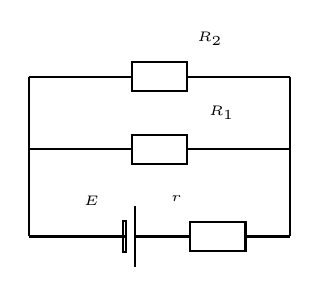
\begin{tikzpicture}[x=0.75pt,y=0.75pt,yscale=-1.4,xscale=1.4]
%uncomment if require: \path (0,300); %set diagram left start at 0, and has height of 300

%Shape: Resistor [id:dp514309969460313] 
\draw   (265.9,120) -- (285.1,120) -- (285.1,130) -- (265.9,130) -- (265.9,120) -- cycle (260.5,125) -- (265.9,125) (285.1,125) -- (290.5,125) ;
%Shape: Battery [id:dp2916012360245832] 
\draw   (230.5,125) -- (244,125) (247,114.36) -- (247,135.64) (247,125) -- (260.5,125) (242.8,119.68) -- (244,119.68) -- (244,130.32) -- (242.8,130.32) -- (242.8,119.68) -- cycle ;
%Straight Lines [id:da2734255254924993] 
\draw    (210.5,70) -- (210.5,125) ;
%Straight Lines [id:da8342089479991157] 
\draw    (300.5,70) -- (300.5,125) ;
%Straight Lines [id:da4571525926989708] 
\draw    (210.5,125) -- (230.5,125) ;
%Straight Lines [id:da08274074907134321] 
\draw    (290.5,125) -- (300.5,125) ;
%Shape: Resistor [id:dp8558892883342235] 
\draw   (245.9,90) -- (265.1,90) -- (265.1,100) -- (245.9,100) -- (245.9,90) -- cycle (240.5,95) -- (245.9,95) (265.1,95) -- (270.5,95) ;
%Straight Lines [id:da7537185022486395] 
\draw    (240.5,95) -- (210.5,95) ;
%Straight Lines [id:da8797643160506492] 
\draw    (300.5,95) -- (270.5,95) ;
%Shape: Resistor [id:dp5429151855494494] 
\draw   (245.9,65) -- (265.1,65) -- (265.1,75) -- (245.9,75) -- (245.9,65) -- cycle (240.5,70) -- (245.9,70) (265.1,70) -- (270.5,70) ;
%Straight Lines [id:da9804503401878168] 
\draw    (240.5,70) -- (210.5,70) ;
%Straight Lines [id:da5427185273385342] 
\draw    (300.5,70) -- (270.5,70) ;

% Text Node
\draw (232.5,108.5) node [anchor=north west][inner sep=0.75pt]   [align=left] {$ $};
% Text Node
\draw (228.5,110) node [anchor=north west][inner sep=0.75pt]  [font=\tiny] [align=left] {$\displaystyle \ms E$};
% Text Node
\draw (258.5,110) node [anchor=north west][inner sep=0.75pt]  [font=\tiny] [align=left] {$\displaystyle r$};
% Text Node
\draw (271.5,79) node [anchor=north west][inner sep=0.75pt]  [font=\tiny] [align=left] {$\displaystyle R_{1}$};
% Text Node
\draw (267.5,53.5) node [anchor=north west][inner sep=0.75pt]  [font=\tiny] [align=left] {$\displaystyle R_{2}$};


\end{tikzpicture}

\end{center}

如果我们想将除了$R_2$外的电路等效为一个电压源,则我们可以使用戴维宁\footnote{有些教材又称其为戴维南定理}(Thevenin)定理(又称等效电压源定理)

\begin{theo}[label=dwndl]{戴维宁定理}{}
对于一个二端有源电路网络,若电路中只有线性元件\footnote{这里线性元件一般指纯电阻,或稳定交流电下的电容和电感(他们在交流电下具有容抗和感抗,可等效为电阻(不考虑相位变化情况下),但在高中一般不要求分析具有容抗和感抗的交流电路,故一般情况下只需考虑纯电阻,对于下文诺顿定理同理},则我们可以将其等效为一个电压源,其\textbf{等效电动势等于两端的开路电压,等效内阻等于去除电动势后两端的电阻}。

这里“二端有源电路网络”中所指的“网络”泛指电路中其中一部分,“有源”指这部分电路中包含电源,“二端”指这段电路只有两个端口。对于下面的诺顿定理同理。
\end{theo}

对于上面的电路,以下标eq\footnote{equivalent的简写}代表等效的值,根据戴维宁定理有

\begin{center}

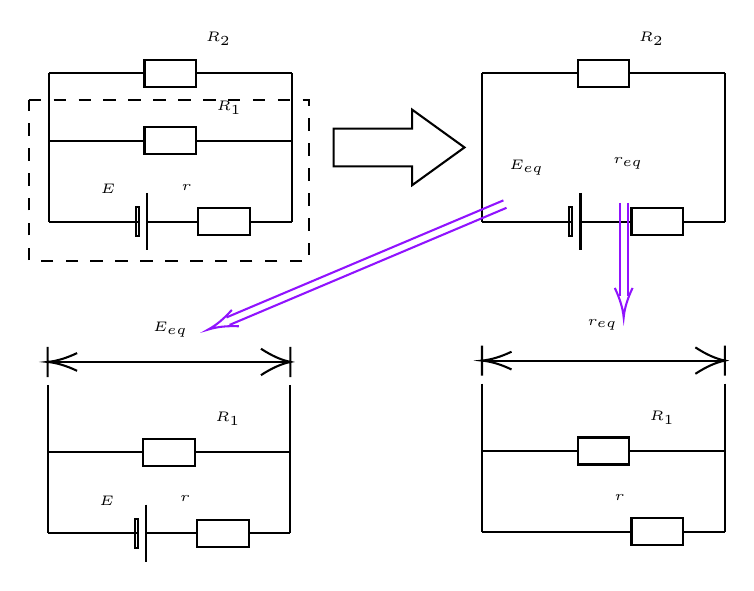
\begin{tikzpicture}[x=0.75pt,y=0.75pt,yscale=-1.3,xscale=1.3]
%uncomment if require: \path (0,300); %set diagram left start at 0, and has height of 300

%Shape: Resistor [id:dp7232411406538839] 
\draw   (245.9,100) -- (265.1,100) -- (265.1,110) -- (245.9,110) -- (245.9,100) -- cycle (240.5,105) -- (245.9,105) (265.1,105) -- (270.5,105) ;
%Shape: Battery [id:dp6693718019533714] 
\draw   (210.5,105) -- (224,105) (227,94.36) -- (227,115.64) (227,105) -- (240.5,105) (222.8,99.68) -- (224,99.68) -- (224,110.32) -- (222.8,110.32) -- (222.8,99.68) -- cycle ;
%Straight Lines [id:da16042882813115766] 
\draw    (190.5,50) -- (190.5,105) ;
%Straight Lines [id:da9402822543750411] 
\draw    (280.5,50) -- (280.5,105) ;
%Straight Lines [id:da12067780236857573] 
\draw    (190.5,105) -- (210.5,105) ;
%Straight Lines [id:da32759114986333504] 
\draw    (270.5,105) -- (280.5,105) ;
%Shape: Resistor [id:dp044708648259699446] 
\draw   (225.9,70) -- (245.1,70) -- (245.1,80) -- (225.9,80) -- (225.9,70) -- cycle (220.5,75) -- (225.9,75) (245.1,75) -- (250.5,75) ;
%Straight Lines [id:da8149590161538551] 
\draw    (220.5,75) -- (190.5,75) ;
%Straight Lines [id:da37292062821096206] 
\draw    (280.5,75) -- (250.5,75) ;
%Shape: Resistor [id:dp8915224058603441] 
\draw   (225.9,45) -- (245.1,45) -- (245.1,55) -- (225.9,55) -- (225.9,45) -- cycle (220.5,50) -- (225.9,50) (245.1,50) -- (250.5,50) ;
%Straight Lines [id:da8050738969027882] 
\draw    (220.5,50) -- (190.5,50) ;
%Straight Lines [id:da41847017454589475] 
\draw    (280.5,50) -- (250.5,50) ;
%Shape: Resistor [id:dp8946522623697388] 
\draw   (406.4,100) -- (425.6,100) -- (425.6,110) -- (406.4,110) -- (406.4,100) -- cycle (401,105) -- (406.4,105) (425.6,105) -- (431,105) ;
%Shape: Battery [id:dp4946459974897708] 
\draw   (371,105) -- (384.5,105) (387.5,94.36) -- (387.5,115.64) (387.5,105) -- (401,105) (383.3,99.68) -- (384.5,99.68) -- (384.5,110.32) -- (383.3,110.32) -- (383.3,99.68) -- cycle ;
%Straight Lines [id:da8491657091150393] 
\draw    (351,50) -- (351,105) ;
%Straight Lines [id:da8293033184283518] 
\draw    (441,50) -- (441,105) ;
%Straight Lines [id:da6903389383039646] 
\draw    (351,105) -- (371,105) ;
%Straight Lines [id:da4919692394445716] 
\draw    (431,105) -- (441,105) ;
%Shape: Resistor [id:dp9226843247374981] 
\draw   (386.4,45) -- (405.6,45) -- (405.6,55) -- (386.4,55) -- (386.4,45) -- cycle (381,50) -- (386.4,50) (405.6,50) -- (411,50) ;
%Straight Lines [id:da5240532491363821] 
\draw    (381,50) -- (351,50) ;
%Straight Lines [id:da8200773875832033] 
\draw    (441,50) -- (411,50) ;
%Right Arrow [id:dp12563132066413996] 
\draw   (296,70.5) -- (325.1,70.5) -- (325.1,63.5) -- (344.5,77.5) -- (325.1,91.5) -- (325.1,84.5) -- (296,84.5) -- cycle ;
%Shape: Rectangle [id:dp8119351522330263] 
\draw  [dash pattern={on 4.5pt off 4.5pt}] (183,60) -- (287,60) -- (287,119.5) -- (183,119.5) -- cycle ;
%Shape: Resistor [id:dp9181595801961024] 
\draw   (245.4,215.5) -- (264.6,215.5) -- (264.6,225.5) -- (245.4,225.5) -- (245.4,215.5) -- cycle (240,220.5) -- (245.4,220.5) (264.6,220.5) -- (270,220.5) ;
%Shape: Battery [id:dp8638451126944211] 
\draw   (210,220.5) -- (223.5,220.5) (226.5,209.86) -- (226.5,231.14) (226.5,220.5) -- (240,220.5) (222.3,215.18) -- (223.5,215.18) -- (223.5,225.82) -- (222.3,225.82) -- (222.3,215.18) -- cycle ;
%Straight Lines [id:da9493469917798139] 
\draw    (190,165.5) -- (190,220.5) ;
%Straight Lines [id:da9469350410050841] 
\draw    (280,165.5) -- (280,220.5) ;
%Straight Lines [id:da9707422227961422] 
\draw    (190,220.5) -- (210,220.5) ;
%Straight Lines [id:da47902505858245004] 
\draw    (270,220.5) -- (280,220.5) ;
%Shape: Resistor [id:dp44228410120226136] 
\draw   (225.4,185.5) -- (244.6,185.5) -- (244.6,195.5) -- (225.4,195.5) -- (225.4,185.5) -- cycle (220,190.5) -- (225.4,190.5) (244.6,190.5) -- (250,190.5) ;
%Straight Lines [id:da7513382191815712] 
\draw    (220,190.5) -- (190,190.5) ;
%Straight Lines [id:da4997577437287888] 
\draw    (280,190.5) -- (250,190.5) ;
%Straight Lines [id:da29586923725139136] 
\draw    (190,157) -- (280,157) ;
\draw [shift={(280,157)}, rotate = 180] [color={rgb, 255:red, 0; green, 0; blue, 0 }  ][line width=0.75]    (0,5.59) -- (0,-5.59)(10.93,-4.9) .. controls (6.95,-2.3) and (3.31,-0.67) .. (0,0) .. controls (3.31,0.67) and (6.95,2.3) .. (10.93,4.9)   ;
\draw [shift={(190,157)}, rotate = 0] [color={rgb, 255:red, 0; green, 0; blue, 0 }  ][line width=0.75]    (0,5.59) -- (0,-5.59)(10.93,-3.29) .. controls (6.95,-1.4) and (3.31,-0.3) .. (0,0) .. controls (3.31,0.3) and (6.95,1.4) .. (10.93,3.29)   ;
%Shape: Resistor [id:dp0668394417226108] 
\draw   (406.4,215) -- (425.6,215) -- (425.6,225) -- (406.4,225) -- (406.4,215) -- cycle (401,220) -- (406.4,220) (425.6,220) -- (431,220) ;
%Straight Lines [id:da585027680617425] 
\draw    (351,165) -- (351,220) ;
%Straight Lines [id:da24202593084033786] 
\draw    (441,165) -- (441,220) ;
%Straight Lines [id:da7950606810490672] 
\draw    (351,220) -- (401,220) ;
%Straight Lines [id:da9338085769888853] 
\draw    (431,220) -- (441,220) ;
%Shape: Resistor [id:dp9351098294796791] 
\draw   (386.4,185) -- (405.6,185) -- (405.6,195) -- (386.4,195) -- (386.4,185) -- cycle (381,190) -- (386.4,190) (405.6,190) -- (411,190) ;
%Straight Lines [id:da7426770619592475] 
\draw    (381,190) -- (351,190) ;
%Straight Lines [id:da4939519386694273] 
\draw    (441,190) -- (411,190) ;
%Straight Lines [id:da5374904022522706] 
\draw    (351,156.5) -- (441,156.5) ;
\draw [shift={(441,156.5)}, rotate = 180] [color={rgb, 255:red, 0; green, 0; blue, 0 }  ][line width=0.75]    (0,5.59) -- (0,-5.59)(10.93,-4.9) .. controls (6.95,-2.3) and (3.31,-0.67) .. (0,0) .. controls (3.31,0.67) and (6.95,2.3) .. (10.93,4.9)   ;
\draw [shift={(351,156.5)}, rotate = 0] [color={rgb, 255:red, 0; green, 0; blue, 0 }  ][line width=0.75]    (0,5.59) -- (0,-5.59)(10.93,-3.29) .. controls (6.95,-1.4) and (3.31,-0.3) .. (0,0) .. controls (3.31,0.3) and (6.95,1.4) .. (10.93,3.29)   ;
%Straight Lines [id:da48480372543600314] 
\draw [color={rgb, 255:red, 144; green, 19; blue, 254 }  ,draw opacity=1 ]   (360.08,99.88) -- (257.45,143.27)(358.92,97.12) -- (256.28,140.5) ;
\draw [shift={(249.5,145)}, rotate = 337.08] [color={rgb, 255:red, 144; green, 19; blue, 254 }  ,draw opacity=1 ][line width=0.75]    (10.93,-3.29) .. controls (6.95,-1.4) and (3.31,-0.3) .. (0,0) .. controls (3.31,0.3) and (6.95,1.4) .. (10.93,3.29)   ;
%Straight Lines [id:da6108098931367383] 
\draw [color={rgb, 255:red, 144; green, 19; blue, 254 }  ,draw opacity=1 ]   (405,98) -- (405,132.5)(402,98) -- (402,132.5) ;
\draw [shift={(403.5,140.5)}, rotate = 270] [color={rgb, 255:red, 144; green, 19; blue, 254 }  ,draw opacity=1 ][line width=0.75]    (10.93,-3.29) .. controls (6.95,-1.4) and (3.31,-0.3) .. (0,0) .. controls (3.31,0.3) and (6.95,1.4) .. (10.93,3.29)   ;

% Text Node
\draw (212.5,88.5) node [anchor=north west][inner sep=0.75pt]   [align=left] {$ $};
% Text Node
\draw (208.5,90) node [anchor=north west][inner sep=0.75pt]  [font=\tiny] [align=left] {$\displaystyle \ms E$};
% Text Node
\draw (238.5,90) node [anchor=north west][inner sep=0.75pt]  [font=\tiny] [align=left] {$\displaystyle r$};
% Text Node
\draw (251.5,59) node [anchor=north west][inner sep=0.75pt]  [font=\tiny] [align=left] {$\displaystyle R_{1}$};
% Text Node
\draw (247.5,33.5) node [anchor=north west][inner sep=0.75pt]  [font=\tiny] [align=left] {$\displaystyle R_{2}$};
% Text Node
\draw (373,88.5) node [anchor=north west][inner sep=0.75pt]   [align=left] {$ $};
% Text Node
\draw (360,81) node [anchor=north west][inner sep=0.75pt]  [font=\tiny] [align=left] {$\displaystyle \ms E_{eq}$};
% Text Node
\draw (398.5,80) node [anchor=north west][inner sep=0.75pt]  [font=\tiny] [align=left] {$\displaystyle r_{eq}$};
% Text Node
\draw (408,33.5) node [anchor=north west][inner sep=0.75pt]  [font=\tiny] [align=left] {$\displaystyle R_{2}$};
% Text Node
\draw (212,204) node [anchor=north west][inner sep=0.75pt]   [align=left] {$ $};
% Text Node
\draw (208,205.5) node [anchor=north west][inner sep=0.75pt]  [font=\tiny] [align=left] {$\displaystyle \ms E$};
% Text Node
\draw (238,205.5) node [anchor=north west][inner sep=0.75pt]  [font=\tiny] [align=left] {$\displaystyle r$};
% Text Node
\draw (251,174.5) node [anchor=north west][inner sep=0.75pt]  [font=\tiny] [align=left] {$\displaystyle R_{1}$};
% Text Node
\draw (228,141) node [anchor=north west][inner sep=0.75pt]  [font=\tiny] [align=left] {$\displaystyle \ms E_{eq}$};
% Text Node
\draw (399,205) node [anchor=north west][inner sep=0.75pt]  [font=\tiny] [align=left] {$\displaystyle r$};
% Text Node
\draw (412,174) node [anchor=north west][inner sep=0.75pt]  [font=\tiny] [align=left] {$\displaystyle R_{1}$};
% Text Node
\draw (389,140) node [anchor=north west][inner sep=0.75pt]  [font=\tiny] [align=left] {$\displaystyle r_{eq}$};


\end{tikzpicture}

\end{center}

\begin{subequations}
\begin{align*}
\ms E_{eq} &= \frac{\ms E R_1}{r + R_1} \\
r_{eq} &= \frac{r R_1}{r + R_1}
\end{align*}
\end{subequations}

同理,如果我们想将除了$R_2$外的电路等效为一个电压源,则我们可以使用诺顿(Norton)定理(又称等效电流源定理)

\begin{theo}{诺顿定理}{}
对于一个二端有源电路网络,若电路中只有线性元件,则我们可以将其等效为一个电流源,其\textbf{等效理想电流源电流等于两端短路时电流,等效内阻等于去除电动势后两端的电阻}。
\end{theo}

对于上面的电路,以下标eq代表等效的值,根据诺顿定理有

\begin{center}
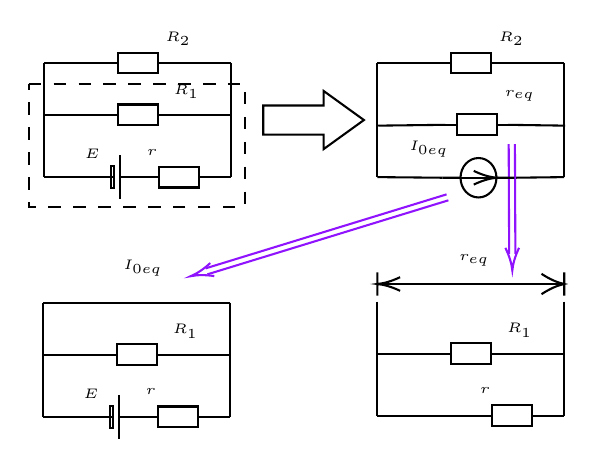
\begin{tikzpicture}[x=0.75pt,y=0.75pt,yscale=-1,xscale=1]
%uncomment if require: \path (0,300); %set diagram left start at 0, and has height of 300

%Shape: Resistor [id:dp7232411406538839] 
\draw   (245.9,100) -- (265.1,100) -- (265.1,110) -- (245.9,110) -- (245.9,100) -- cycle (240.5,105) -- (245.9,105) (265.1,105) -- (270.5,105) ;
%Shape: Battery [id:dp6693718019533714] 
\draw   (210.5,105) -- (224,105) (227,94.36) -- (227,115.64) (227,105) -- (240.5,105) (222.8,99.68) -- (224,99.68) -- (224,110.32) -- (222.8,110.32) -- (222.8,99.68) -- cycle ;
%Straight Lines [id:da16042882813115766] 
\draw    (190.5,50) -- (190.5,105) ;
%Straight Lines [id:da9402822543750411] 
\draw    (280.5,50) -- (280.5,105) ;
%Straight Lines [id:da12067780236857573] 
\draw    (190.5,105) -- (210.5,105) ;
%Straight Lines [id:da32759114986333504] 
\draw    (270.5,105) -- (280.5,105) ;
%Shape: Resistor [id:dp044708648259699446] 
\draw   (225.9,70) -- (245.1,70) -- (245.1,80) -- (225.9,80) -- (225.9,70) -- cycle (220.5,75) -- (225.9,75) (245.1,75) -- (250.5,75) ;
%Straight Lines [id:da8149590161538551] 
\draw    (220.5,75) -- (190.5,75) ;
%Straight Lines [id:da37292062821096206] 
\draw    (280.5,75) -- (250.5,75) ;
%Shape: Resistor [id:dp8915224058603441] 
\draw   (225.9,45) -- (245.1,45) -- (245.1,55) -- (225.9,55) -- (225.9,45) -- cycle (220.5,50) -- (225.9,50) (245.1,50) -- (250.5,50) ;
%Straight Lines [id:da8050738969027882] 
\draw    (220.5,50) -- (190.5,50) ;
%Straight Lines [id:da41847017454589475] 
\draw    (280.5,50) -- (250.5,50) ;
%Shape: Resistor [id:dp8946522623697388] 
\draw   (389.2,74.8) -- (408.4,74.8) -- (408.4,84.8) -- (389.2,84.8) -- (389.2,74.8) -- cycle (383.8,79.8) -- (389.2,79.8) (408.4,79.8) -- (413.8,79.8) ;
%Straight Lines [id:da8491657091150393] 
\draw    (351,50) -- (351,105) ;
%Straight Lines [id:da8293033184283518] 
\draw    (441,50) -- (441,105) ;
%Straight Lines [id:da6903389383039646] 
\draw    (351,105) -- (382.4,105.3) ;
%Straight Lines [id:da4919692394445716] 
\draw    (417,105.3) -- (441,105) ;
%Shape: Resistor [id:dp9226843247374981] 
\draw   (386.4,45) -- (405.6,45) -- (405.6,55) -- (386.4,55) -- (386.4,45) -- cycle (381,50) -- (386.4,50) (405.6,50) -- (411,50) ;
%Straight Lines [id:da5240532491363821] 
\draw    (381,50) -- (351,50) ;
%Straight Lines [id:da8200773875832033] 
\draw    (441,50) -- (411,50) ;
%Right Arrow [id:dp12563132066413996] 
\draw   (296,70.5) -- (325.1,70.5) -- (325.1,63.5) -- (344.5,77.5) -- (325.1,91.5) -- (325.1,84.5) -- (296,84.5) -- cycle ;
%Shape: Rectangle [id:dp8119351522330263] 
\draw  [dash pattern={on 4.5pt off 4.5pt}] (183,60) -- (287,60) -- (287,119.5) -- (183,119.5) -- cycle ;
%Shape: Resistor [id:dp9181595801961024] 
\draw   (245.4,215.5) -- (264.6,215.5) -- (264.6,225.5) -- (245.4,225.5) -- (245.4,215.5) -- cycle (240,220.5) -- (245.4,220.5) (264.6,220.5) -- (270,220.5) ;
%Shape: Battery [id:dp8638451126944211] 
\draw   (210,220.5) -- (223.5,220.5) (226.5,209.86) -- (226.5,231.14) (226.5,220.5) -- (240,220.5) (222.3,215.18) -- (223.5,215.18) -- (223.5,225.82) -- (222.3,225.82) -- (222.3,215.18) -- cycle ;
%Straight Lines [id:da9493469917798139] 
\draw    (190,165.5) -- (190,220.5) ;
%Straight Lines [id:da9469350410050841] 
\draw    (280,165.5) -- (280,220.5) ;
%Straight Lines [id:da9707422227961422] 
\draw    (190,220.5) -- (210,220.5) ;
%Straight Lines [id:da47902505858245004] 
\draw    (270,220.5) -- (280,220.5) ;
%Shape: Resistor [id:dp44228410120226136] 
\draw   (225.4,185.5) -- (244.6,185.5) -- (244.6,195.5) -- (225.4,195.5) -- (225.4,185.5) -- cycle (220,190.5) -- (225.4,190.5) (244.6,190.5) -- (250,190.5) ;
%Straight Lines [id:da7513382191815712] 
\draw    (220,190.5) -- (190,190.5) ;
%Straight Lines [id:da4997577437287888] 
\draw    (280,190.5) -- (250,190.5) ;
%Shape: Resistor [id:dp0668394417226108] 
\draw   (406.4,215) -- (425.6,215) -- (425.6,225) -- (406.4,225) -- (406.4,215) -- cycle (401,220) -- (406.4,220) (425.6,220) -- (431,220) ;
%Straight Lines [id:da585027680617425] 
\draw    (351,165) -- (351,220) ;
%Straight Lines [id:da24202593084033786] 
\draw    (441,165) -- (441,220) ;
%Straight Lines [id:da7950606810490672] 
\draw    (351,220) -- (401,220) ;
%Straight Lines [id:da9338085769888853] 
\draw    (431,220) -- (441,220) ;
%Shape: Resistor [id:dp9351098294796791] 
\draw   (386.4,185) -- (405.6,185) -- (405.6,195) -- (386.4,195) -- (386.4,185) -- cycle (381,190) -- (386.4,190) (405.6,190) -- (411,190) ;
%Straight Lines [id:da7426770619592475] 
\draw    (381,190) -- (351,190) ;
%Straight Lines [id:da4939519386694273] 
\draw    (441,190) -- (411,190) ;
%Straight Lines [id:da5374904022522706] 
\draw    (351,156.5) -- (441,156.5) ;
\draw [shift={(441,156.5)}, rotate = 180] [color={rgb, 255:red, 0; green, 0; blue, 0 }  ][line width=0.75]    (0,5.59) -- (0,-5.59)(10.93,-4.9) .. controls (6.95,-2.3) and (3.31,-0.67) .. (0,0) .. controls (3.31,0.67) and (6.95,2.3) .. (10.93,4.9)   ;
\draw [shift={(351,156.5)}, rotate = 0] [color={rgb, 255:red, 0; green, 0; blue, 0 }  ][line width=0.75]    (0,5.59) -- (0,-5.59)(10.93,-3.29) .. controls (6.95,-1.4) and (3.31,-0.3) .. (0,0) .. controls (3.31,0.3) and (6.95,1.4) .. (10.93,3.29)   ;
%Straight Lines [id:da48480372543600314] 
\draw [color={rgb, 255:red, 144; green, 19; blue, 254 }  ,draw opacity=1 ]   (385.19,116.18) -- (269.09,151.84)(384.31,113.32) -- (268.21,148.97) ;
\draw [shift={(261,152.75)}, rotate = 342.93] [color={rgb, 255:red, 144; green, 19; blue, 254 }  ,draw opacity=1 ][line width=0.75]    (10.93,-3.29) .. controls (6.95,-1.4) and (3.31,-0.3) .. (0,0) .. controls (3.31,0.3) and (6.95,1.4) .. (10.93,3.29)   ;
%Straight Lines [id:da6108098931367383] 
\draw [color={rgb, 255:red, 144; green, 19; blue, 254 }  ,draw opacity=1 ]   (417.25,89.09) -- (417.47,141.99)(414.25,89.11) -- (414.47,142.01) ;
\draw [shift={(416,150)}, rotate = 269.76] [color={rgb, 255:red, 144; green, 19; blue, 254 }  ,draw opacity=1 ][line width=0.75]    (10.93,-3.29) .. controls (6.95,-1.4) and (3.31,-0.3) .. (0,0) .. controls (3.31,0.3) and (6.95,1.4) .. (10.93,3.29)   ;
%Shape: Output [id:dp3254919178538347] 
\draw   (391.05,105.3) .. controls (391.05,100.05) and (394.92,95.8) .. (399.7,95.8) .. controls (404.48,95.8) and (408.35,100.05) .. (408.35,105.3) .. controls (408.35,110.55) and (404.48,114.8) .. (399.7,114.8) .. controls (394.92,114.8) and (391.05,110.55) .. (391.05,105.3) -- cycle (382.4,105.3) -- (391.05,105.3) (417,105.3) -- (408.35,105.3) ;
%Straight Lines [id:da2727693576449006] 
\draw    (391.05,105.3) -- (406.35,105.3) ;
\draw [shift={(408.35,105.3)}, rotate = 180] [color={rgb, 255:red, 0; green, 0; blue, 0 }  ][line width=0.75]    (10.93,-3.29) .. controls (6.95,-1.4) and (3.31,-0.3) .. (0,0) .. controls (3.31,0.3) and (6.95,1.4) .. (10.93,3.29)   ;
%Straight Lines [id:da028581311463260928] 
\draw    (351.4,80.2) -- (383.8,79.8) ;
%Straight Lines [id:da8344804917733968] 
\draw    (413.8,79.8) -- (441.4,80.2) ;
%Straight Lines [id:da8732003928059893] 
\draw    (190,165.5) -- (280,165.5) ;

% Text Node
\draw (212.5,88.5) node [anchor=north west][inner sep=0.75pt]   [align=left] {$ $};
% Text Node
\draw (208.5,90) node [anchor=north west][inner sep=0.75pt]  [font=\tiny] [align=left] {$\displaystyle \ms E$};
% Text Node
\draw (238.5,90) node [anchor=north west][inner sep=0.75pt]  [font=\tiny] [align=left] {$\displaystyle r$};
% Text Node
\draw (251.5,59) node [anchor=north west][inner sep=0.75pt]  [font=\tiny] [align=left] {$\displaystyle R_{1}$};
% Text Node
\draw (247.5,33.5) node [anchor=north west][inner sep=0.75pt]  [font=\tiny] [align=left] {$\displaystyle R_{2}$};
% Text Node
\draw (410.95,61.6) node [anchor=north west][inner sep=0.75pt]  [font=\tiny] [align=left] {$\displaystyle r_{eq}$};
% Text Node
\draw (408,33.5) node [anchor=north west][inner sep=0.75pt]  [font=\tiny] [align=left] {$\displaystyle R_{2}$};
% Text Node
\draw (212,204) node [anchor=north west][inner sep=0.75pt]   [align=left] {$ $};
% Text Node
\draw (208,205.5) node [anchor=north west][inner sep=0.75pt]  [font=\tiny] [align=left] {$\displaystyle \ms E$};
% Text Node
\draw (238,205.5) node [anchor=north west][inner sep=0.75pt]  [font=\tiny] [align=left] {$\displaystyle r$};
% Text Node
\draw (251,174.5) node [anchor=north west][inner sep=0.75pt]  [font=\tiny] [align=left] {$\displaystyle R_{1}$};
% Text Node
\draw (227.25,143.5) node [anchor=north west][inner sep=0.75pt]  [font=\tiny] [align=left] {$\displaystyle I_{0eq}$};
% Text Node
\draw (399,205) node [anchor=north west][inner sep=0.75pt]  [font=\tiny] [align=left] {$\displaystyle r$};
% Text Node
\draw (412,174) node [anchor=north west][inner sep=0.75pt]  [font=\tiny] [align=left] {$\displaystyle R_{1}$};
% Text Node
\draw (389,140.75) node [anchor=north west][inner sep=0.75pt]  [font=\tiny] [align=left] {$\displaystyle r_{eq}$};
% Text Node
\draw (365,86.25) node [anchor=north west][inner sep=0.75pt]  [font=\tiny] [align=left] {$\displaystyle I_{0eq}$};


\end{tikzpicture}
\end{center}

\begin{subequations}
\begin{align*}
I_{0 eq} &= \frac{\ms E}{r} \\
r_{eq} &= \frac{r R_1}{r + R_1}
\end{align*}
\end{subequations}

\begin{mk}{思考}{}
试运用前文\theoref{dyydlygx} 证明戴维宁定理跟诺顿定理的等效性。
\end{mk}

在高考中,戴维宁定理可以帮助我们快速分析出电学实验题中的误差,而诺顿定理在高考中运用的较少,但为了论述的完整,故仍旧介绍了诺顿定理。一般而言能够熟练运用戴维宁定理即可。

\subsection{等效源在电路分析中作用}

在对闭合电路的一些具体问题的分析之中,运用等效源,通过将电源与电路中的某一部分看为一个整体,将其等效为一个新的电源,可使问题的分析变得清晰,求解过程变得简单。

\begin{ep}{自编题}{}
试分别分析测量电池电动势时内接法和外接法测量值与实际值偏大还是偏小?

~\\
\textbf{由于电表存在内阻,我们可以认为电表就是一个可以显示其电压或电流的电阻,将其分为理想电表和内阻的串并联}。由此易知,\textbf{对于电压表,其可等效为内阻与理想电压表并联;对于电流表,其可等效为内阻与理想电流表串联}。

对于内接法,我们将影响测量的内侧的电流表进行等效,其电路图以及等效电路图如图所示:

\begin{center}
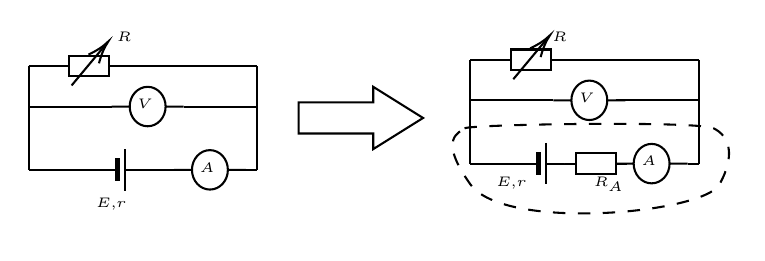
\begin{tikzpicture}[x=0.75pt,y=0.75pt,yscale=-1,xscale=1]
%uncomment if require: \path (0,300); %set diagram left start at 0, and has height of 300

%Straight Lines [id:da9223803374157449] 
\draw    (200,160) -- (230,160) ;
%Straight Lines [id:da4800046187933087] 
\draw    (310,129.5) -- (280,129.5) ;
%Shape: Battery [id:dp11572428456821915] 
\draw   (230,160) -- (243.5,160) (246.5,150) -- (246.5,170) (246.5,160) -- (260,160) (242.3,155) -- (243.5,155) -- (243.5,165) -- (242.3,165) -- (242.3,155) -- cycle ;
%Straight Lines [id:da5053925872800769] 
\draw    (200,110) -- (200,160) ;
%Straight Lines [id:da4775642533714568] 
\draw    (304.6,160) -- (310,160) ;
%Straight Lines [id:da025516599512321214] 
\draw    (310,110) -- (310,160) ;
%Shape: Output [id:dp20535874065942084] 
\draw   (278.65,160) .. controls (278.65,154.75) and (282.52,150.5) .. (287.3,150.5) .. controls (292.08,150.5) and (295.95,154.75) .. (295.95,160) .. controls (295.95,165.25) and (292.08,169.5) .. (287.3,169.5) .. controls (282.52,169.5) and (278.65,165.25) .. (278.65,160) -- cycle (270,160) -- (278.65,160) (304.6,160) -- (295.95,160) ;
%Straight Lines [id:da8691520573396538] 
\draw    (260,160) -- (270,160) ;
%Straight Lines [id:da22747916883790165] 
\draw    (200,110) -- (214,110) ;
%Shape: Resistor [id:dp2800596618552471] 
\draw   (219.4,115) -- (238.6,115) -- (238.6,105) -- (219.4,105) -- (219.4,115) -- cycle (214,110) -- (219.4,110) (238.6,110) -- (244,110) ;
%Straight Lines [id:da15708168083551777] 
\draw    (220.67,119.33) -- (237.04,99.7) ;
\draw [shift={(238.33,98.16)}, rotate = 129.83] [color={rgb, 255:red, 0; green, 0; blue, 0 }  ][line width=0.75]    (10.93,-3.29) .. controls (6.95,-1.4) and (3.31,-0.3) .. (0,0) .. controls (3.31,0.3) and (6.95,1.4) .. (10.93,3.29)   ;

%Straight Lines [id:da11312699458388331] 
\draw    (244,110) -- (310,110) ;
%Straight Lines [id:da6739961140053903] 
\draw    (274.6,129.5) -- (280,129.5) ;
%Shape: Output [id:dp7899198086186321] 
\draw   (248.65,129.5) .. controls (248.65,124.25) and (252.52,120) .. (257.3,120) .. controls (262.08,120) and (265.95,124.25) .. (265.95,129.5) .. controls (265.95,134.75) and (262.08,139) .. (257.3,139) .. controls (252.52,139) and (248.65,134.75) .. (248.65,129.5) -- cycle (240,129.5) -- (248.65,129.5) (274.6,129.5) -- (265.95,129.5) ;
%Straight Lines [id:da613270518508825] 
\draw    (230,129.5) -- (240,129.5) ;
%Straight Lines [id:da16840770867474064] 
\draw    (230,129.5) -- (200,129.5) ;
%Right Arrow [id:dp7706619739903626] 
\draw   (330,127.5) -- (366,127.5) -- (366,120) -- (390,135) -- (366,150) -- (366,142.5) -- (330,142.5) -- cycle ;
%Straight Lines [id:da4168340291806618] 
\draw    (412.81,157) -- (432.81,157) ;
%Shape: Battery [id:dp07811227108971108] 
\draw   (432.81,157) -- (446.31,157) (449.31,147) -- (449.31,167) (449.31,157) -- (462.81,157) (445.11,152) -- (446.31,152) -- (446.31,162) -- (445.11,162) -- (445.11,152) -- cycle ;
%Straight Lines [id:da5277780096339191] 
\draw    (412.81,107) -- (412.81,157) ;
%Straight Lines [id:da6252032764865012] 
\draw    (517.41,157) -- (522.81,157) ;
%Straight Lines [id:da2775418013876463] 
\draw    (522.81,107) -- (522.81,157) ;
%Shape: Output [id:dp4334794925404719] 
\draw   (491.46,157) .. controls (491.46,151.75) and (495.33,147.5) .. (500.11,147.5) .. controls (504.88,147.5) and (508.76,151.75) .. (508.76,157) .. controls (508.76,162.25) and (504.88,166.5) .. (500.11,166.5) .. controls (495.33,166.5) and (491.46,162.25) .. (491.46,157) -- cycle (482.81,157) -- (491.46,157) (517.41,157) -- (508.76,157) ;
%Straight Lines [id:da012898191912185553] 
\draw    (412.81,107) -- (426.81,107) ;
%Shape: Resistor [id:dp43127197925661176] 
\draw   (432.21,112) -- (451.41,112) -- (451.41,102) -- (432.21,102) -- (432.21,112) -- cycle (426.81,107) -- (432.21,107) (451.41,107) -- (456.81,107) ;
%Straight Lines [id:da20629449411629652] 
\draw    (433.47,116.33) -- (449.85,96.7) ;
\draw [shift={(451.13,95.16)}, rotate = 129.83] [color={rgb, 255:red, 0; green, 0; blue, 0 }  ][line width=0.75]    (10.93,-3.29) .. controls (6.95,-1.4) and (3.31,-0.3) .. (0,0) .. controls (3.31,0.3) and (6.95,1.4) .. (10.93,3.29)   ;

%Straight Lines [id:da4199064010002851] 
\draw    (456.81,107) -- (522.81,107) ;
%Straight Lines [id:da025073331712180957] 
\draw    (482.81,126.5) -- (516.81,126.5) ;
%Shape: Output [id:dp8875989383892691] 
\draw   (461.46,126.5) .. controls (461.46,121.25) and (465.33,117) .. (470.11,117) .. controls (474.88,117) and (478.76,121.25) .. (478.76,126.5) .. controls (478.76,131.75) and (474.88,136) .. (470.11,136) .. controls (465.33,136) and (461.46,131.75) .. (461.46,126.5) -- cycle (452.81,126.5) -- (461.46,126.5) (487.41,126.5) -- (478.76,126.5) ;
%Straight Lines [id:da808640618957692] 
\draw    (442.81,126.5) -- (452.81,126.5) ;
%Straight Lines [id:da3805424335033789] 
\draw    (442.81,126.5) -- (412.81,126.5) ;
%Shape: Resistor [id:dp27249147366061965] 
\draw  [color={rgb, 255:red, 0; green, 0; blue, 0 }  ,draw opacity=1 ][fill={rgb, 255:red, 255; green, 255; blue, 255 }  ,fill opacity=1 ][line width=0.75]  (463.61,152) -- (482.81,152) -- (482.81,162) -- (463.61,162) -- (463.61,152) -- cycle (458.21,157) -- (463.61,157) (482.81,157) -- (488.21,157) ;
%Straight Lines [id:da5032822234989214] 
\draw    (516.81,126.5) -- (522.81,126.5) ;
%Shape: Polygon Curved [id:ds2894822220000477] 
\draw  [dash pattern={on 4.5pt off 4.5pt}] (410,140) .. controls (412,138.09) and (522.33,136.25) .. (530,140) .. controls (537.67,143.75) and (540.61,152.91) .. (532.81,167) .. controls (525,181.09) and (429.14,189.75) .. (412.81,167) .. controls (396.47,144.25) and (408,141.91) .. (410,140) -- cycle ;

% Text Node
\draw (281,155) node [anchor=north west][inner sep=0.75pt]  [font=\tiny] [align=left] {$\displaystyle A$};
% Text Node
\draw (251,124.5) node [anchor=north west][inner sep=0.75pt]  [font=\tiny] [align=left] {$\displaystyle V$};
% Text Node
\draw (493.81,152) node [anchor=north west][inner sep=0.75pt]  [font=\tiny] [align=left] {$\displaystyle A$};
% Text Node
\draw (463.81,121.5) node [anchor=north west][inner sep=0.75pt]  [font=\tiny] [align=left] {$\displaystyle V$};
% Text Node
\draw (231,172) node [anchor=north west][inner sep=0.75pt]  [font=\tiny] [align=left] {$\displaystyle \ms E$,$\displaystyle r$};
% Text Node
\draw (241,92) node [anchor=north west][inner sep=0.75pt]  [font=\tiny] [align=left] {$\displaystyle R$};
% Text Node
\draw (450.81,92) node [anchor=north west][inner sep=0.75pt]  [font=\tiny] [align=left] {$\displaystyle R$};
% Text Node
\draw (423.81,162) node [anchor=north west][inner sep=0.75pt]  [font=\tiny] [align=left] {$\displaystyle \ms E$,$\displaystyle r$};
% Text Node
\draw (470.81,162) node [anchor=north west][inner sep=0.75pt]  [font=\tiny] [align=left] {$\displaystyle R_{A}$};
\end{tikzpicture}
\end{center}

将电源及其内阻和电流表内阻等效成新电源,则根据\theoref{dwndl},新电源电动势及内阻为
$$ \ms E^{\prime} = \ms E ,\quad r^{\prime} = r + R_A $$

因此\textbf{电动势测量值与真实值相等,内阻测量值比真实值偏大。}

同理,对于外界法,我们将影响测量的内侧的电压表进行等效,其电路图及等效电路图如图所示

\begin{center}
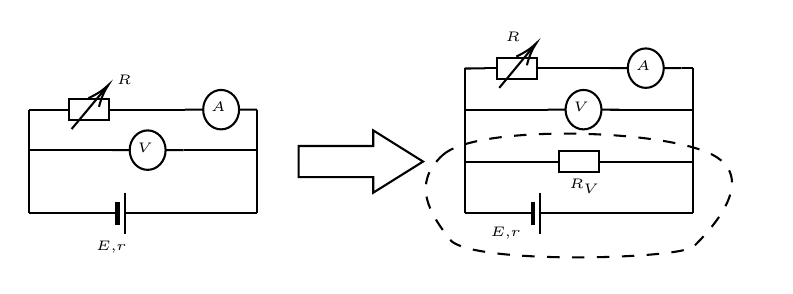
\begin{tikzpicture}[x=0.75pt,y=0.75pt,yscale=-1,xscale=1]
%uncomment if require: \path (0,300); %set diagram left start at 0, and has height of 300

%Straight Lines [id:da9223803374157449] 
\draw    (200,160) -- (230,160) ;
%Straight Lines [id:da4800046187933087] 
\draw    (310,129.5) -- (280,129.5) ;
%Shape: Battery [id:dp11572428456821915] 
\draw   (230,160) -- (243.5,160) (246.5,150) -- (246.5,170) (246.5,160) -- (260,160) (242.3,155) -- (243.5,155) -- (243.5,165) -- (242.3,165) -- (242.3,155) -- cycle ;
%Straight Lines [id:da5053925872800769] 
\draw    (200,110) -- (200,160) ;
%Straight Lines [id:da4775642533714568] 
\draw    (260,160) -- (310,160) ;
%Straight Lines [id:da025516599512321214] 
\draw    (310,110) -- (310,160) ;
%Shape: Output [id:dp20535874065942084] 
\draw   (284.05,110) .. controls (284.05,104.75) and (287.92,100.5) .. (292.7,100.5) .. controls (297.48,100.5) and (301.35,104.75) .. (301.35,110) .. controls (301.35,115.25) and (297.48,119.5) .. (292.7,119.5) .. controls (287.92,119.5) and (284.05,115.25) .. (284.05,110) -- cycle (275.4,110) -- (284.05,110) (310,110) -- (301.35,110) ;
%Straight Lines [id:da22747916883790165] 
\draw    (200,110) -- (214,110) ;
%Shape: Resistor [id:dp2800596618552471] 
\draw   (219.4,115) -- (238.6,115) -- (238.6,105) -- (219.4,105) -- (219.4,115) -- cycle (214,110) -- (219.4,110) (238.6,110) -- (244,110) ;
%Straight Lines [id:da15708168083551777] 
\draw    (220.67,119.33) -- (237.04,99.7) ;
\draw [shift={(238.33,98.16)}, rotate = 129.83] [color={rgb, 255:red, 0; green, 0; blue, 0 }  ][line width=0.75]    (10.93,-3.29) .. controls (6.95,-1.4) and (3.31,-0.3) .. (0,0) .. controls (3.31,0.3) and (6.95,1.4) .. (10.93,3.29)   ;

%Straight Lines [id:da11312699458388331] 
\draw    (244,110) -- (275.4,110) ;
%Straight Lines [id:da6739961140053903] 
\draw    (274.6,129.5) -- (280,129.5) ;
%Shape: Output [id:dp7899198086186321] 
\draw   (248.65,129.5) .. controls (248.65,124.25) and (252.52,120) .. (257.3,120) .. controls (262.08,120) and (265.95,124.25) .. (265.95,129.5) .. controls (265.95,134.75) and (262.08,139) .. (257.3,139) .. controls (252.52,139) and (248.65,134.75) .. (248.65,129.5) -- cycle (240,129.5) -- (248.65,129.5) (274.6,129.5) -- (265.95,129.5) ;
%Straight Lines [id:da613270518508825] 
\draw    (230,129.5) -- (240,129.5) ;
%Straight Lines [id:da16840770867474064] 
\draw    (230,129.5) -- (200,129.5) ;
%Right Arrow [id:dp7706619739903626] 
\draw   (330,127.5) -- (366,127.5) -- (366,120) -- (390,135) -- (366,150) -- (366,142.5) -- (330,142.5) -- cycle ;
%Straight Lines [id:da4168340291806618] 
\draw    (410,160) -- (430,160) ;
%Shape: Battery [id:dp07811227108971108] 
\draw   (430,160) -- (443.5,160) (446.5,150) -- (446.5,170) (446.5,160) -- (460,160) (442.3,155) -- (443.5,155) -- (443.5,165) -- (442.3,165) -- (442.3,155) -- cycle ;
%Straight Lines [id:da5277780096339191] 
\draw    (410,90) -- (410,160) ;
%Straight Lines [id:da6252032764865012] 
\draw    (460,160) -- (520,160) ;
%Straight Lines [id:da2775418013876463] 
\draw    (520,90) -- (520,160) ;
%Shape: Output [id:dp4334794925404719] 
\draw   (488.65,90) .. controls (488.65,84.75) and (492.52,80.5) .. (497.3,80.5) .. controls (502.08,80.5) and (505.95,84.75) .. (505.95,90) .. controls (505.95,95.25) and (502.08,99.5) .. (497.3,99.5) .. controls (492.52,99.5) and (488.65,95.25) .. (488.65,90) -- cycle (480,90) -- (488.65,90) (514.6,90) -- (505.95,90) ;
%Straight Lines [id:da012898191912185553] 
\draw    (410,90.19) -- (420,90.06) ;
%Shape: Resistor [id:dp43127197925661176] 
\draw   (425.43,95.12) -- (444.74,95.12) -- (444.74,85) -- (425.43,85) -- (425.43,95.12) -- cycle (420,90.06) -- (425.43,90.06) (444.74,90.06) -- (450.17,90.06) ;
%Straight Lines [id:da20629449411629652] 
\draw    (426.7,99.5) -- (443.19,79.63) ;
\draw [shift={(444.46,78.09)}, rotate = 129.67] [color={rgb, 255:red, 0; green, 0; blue, 0 }  ][line width=0.75]    (10.93,-3.29) .. controls (6.95,-1.4) and (3.31,-0.3) .. (0,0) .. controls (3.31,0.3) and (6.95,1.4) .. (10.93,3.29)   ;

%Straight Lines [id:da4199064010002851] 
\draw    (450,90) -- (480,90) ;
%Straight Lines [id:da025073331712180957] 
\draw    (480,110) -- (520,110) ;
%Shape: Output [id:dp8875989383892691] 
\draw   (458.65,110) .. controls (458.65,104.75) and (462.52,100.5) .. (467.3,100.5) .. controls (472.08,100.5) and (475.95,104.75) .. (475.95,110) .. controls (475.95,115.25) and (472.08,119.5) .. (467.3,119.5) .. controls (462.52,119.5) and (458.65,115.25) .. (458.65,110) -- cycle (450,110) -- (458.65,110) (484.6,110) -- (475.95,110) ;
%Straight Lines [id:da808640618957692] 
\draw    (440,110) -- (450,110) ;
%Straight Lines [id:da3805424335033789] 
\draw    (440,110) -- (410,110) ;
%Shape: Resistor [id:dp27249147366061965] 
\draw  [color={rgb, 255:red, 0; green, 0; blue, 0 }  ,draw opacity=1 ][fill={rgb, 255:red, 255; green, 255; blue, 255 }  ,fill opacity=1 ][line width=0.75]  (455.4,130) -- (474.6,130) -- (474.6,140) -- (455.4,140) -- (455.4,130) -- cycle (450,135) -- (455.4,135) (474.6,135) -- (480,135) ;
%Straight Lines [id:da5032822234989214] 
\draw    (480,135) -- (520,135) ;
%Shape: Polygon Curved [id:ds2894822220000477] 
\draw  [dash pattern={on 4.5pt off 4.5pt}] (399.5,131.84) .. controls (415.01,117.67) and (499.33,119) .. (526.84,130.5) .. controls (554.34,142.01) and (526.84,169.5) .. (520.5,175.84) .. controls (514.17,182.17) and (412.17,184.84) .. (402.84,172.5) .. controls (393.5,160.17) and (384,146) .. (399.5,131.84) -- cycle ;
%Straight Lines [id:da8501291218143447] 
\draw    (410,135) -- (450,135) ;
%Straight Lines [id:da21442590370161208] 
\draw    (514.6,90) -- (520,90) ;

% Text Node
\draw (286.4,105) node [anchor=north west][inner sep=0.75pt]  [font=\tiny] [align=left] {$\displaystyle A$};
% Text Node
\draw (251,124.5) node [anchor=north west][inner sep=0.75pt]  [font=\tiny] [align=left] {$\displaystyle V$};
% Text Node
\draw (491,85.17) node [anchor=north west][inner sep=0.75pt]  [font=\tiny] [align=left] {$\displaystyle A$};
% Text Node
\draw (461,105) node [anchor=north west][inner sep=0.75pt]  [font=\tiny] [align=left] {$\displaystyle V$};
% Text Node
\draw (231,172) node [anchor=north west][inner sep=0.75pt]  [font=\tiny] [align=left] {$\displaystyle \ms E$,$\displaystyle r$};
% Text Node
\draw (241,92) node [anchor=north west][inner sep=0.75pt]  [font=\tiny] [align=left] {$\displaystyle R$};
% Text Node
\draw (428.33,71) node [anchor=north west][inner sep=0.75pt]  [font=\tiny] [align=left] {$\displaystyle R$};
% Text Node
\draw (421,165) node [anchor=north west][inner sep=0.75pt]  [font=\tiny] [align=left] {$\displaystyle \ms E$,$\displaystyle r$};
% Text Node
\draw (459,142) node [anchor=north west][inner sep=0.75pt]  [font=\tiny] [align=left] {$\displaystyle R_{V}$};
\end{tikzpicture}

\end{center}

将电源及其内阻和电压表内阻等效成新电源,则根据\theoref{dwndl},新电源电动势及内阻为
$$ \ms E^{\prime} = \frac{ \ms E R_V}{R_V + r} ,\quad r^{\prime} = \frac{r R_V}{r + R_V} $$

因此\textbf{电动势测量值比真实值偏小,内阻测量值比真实值偏小。}
\end{ep}

对于选择题,若遇到$\frac{\Delta U}{\Delta I}$且其对应的电阻正在变化,则一般情况下可以使用等效源进行等效,其$\frac{\Delta U}{\Delta I}$等于新内阻。具体可见如下例题。

\begin{ep}{练习题}{}

\begin{center}
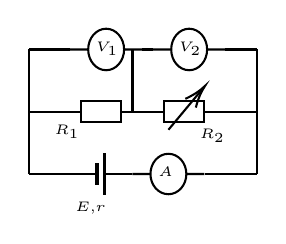
\begin{tikzpicture}[x=0.75pt,y=0.75pt,yscale=-1,xscale=1]
%uncomment if require: \path (0,300); %set diagram left start at 0, and has height of 300

%Straight Lines [id:da14551039289024326] 
\draw    (130,220) -- (150,220) ;
%Straight Lines [id:da3295959610713812] 
\draw    (150,160) -- (130,160) ;
%Shape: Battery [id:dp8317998227732923] 
\draw   (150,220) -- (163.5,220) (166.5,210) -- (166.5,230) (166.5,220) -- (180,220) (162.3,215) -- (163.5,215) -- (163.5,225) -- (162.3,225) -- (162.3,215) -- cycle ;
%Straight Lines [id:da6993800641983081] 
\draw    (130,160) -- (130,220) ;
%Straight Lines [id:da47030402702453067] 
\draw    (215,220) -- (240,220) ;
%Straight Lines [id:da10115275650248856] 
\draw    (240,160) -- (240,220) ;
%Shape: Output [id:dp34471276111404703] 
\draw   (188.65,220) .. controls (188.65,214.62) and (192.52,210.26) .. (197.3,210.26) .. controls (202.08,210.26) and (205.95,214.62) .. (205.95,220) .. controls (205.95,225.38) and (202.08,229.74) .. (197.3,229.74) .. controls (192.52,229.74) and (188.65,225.38) .. (188.65,220) -- cycle (180,220) -- (188.65,220) (214.6,220) -- (205.95,220) ;
%Straight Lines [id:da2535463577123036] 
\draw    (220,190) -- (240,190) ;
%Shape: Resistor [id:dp2889455083490655] 
\draw   (195.4,195) -- (214.6,195) -- (214.6,185) -- (195.4,185) -- (195.4,195) -- cycle (190,190) -- (195.4,190) (214.6,190) -- (220,190) ;
%Straight Lines [id:da6959465546040076] 
\draw    (197.33,198.67) -- (213.71,179.03) ;
\draw [shift={(214.99,177.5)}, rotate = 129.83] [color={rgb, 255:red, 0; green, 0; blue, 0 }  ][line width=0.75]    (10.93,-3.29) .. controls (6.95,-1.4) and (3.31,-0.3) .. (0,0) .. controls (3.31,0.3) and (6.95,1.4) .. (10.93,3.29)   ;
%Straight Lines [id:da7548896744967672] 
\draw    (224.6,160) -- (240,160) ;
%Straight Lines [id:da05255225869571456] 
\draw    (184.6,160) -- (190,160) ;
%Shape: Output [id:dp7402485705608346] 
\draw   (158.65,160) .. controls (158.65,154.48) and (162.52,150) .. (167.3,150) .. controls (172.08,150) and (175.95,154.48) .. (175.95,160) .. controls (175.95,165.52) and (172.08,170) .. (167.3,170) .. controls (162.52,170) and (158.65,165.52) .. (158.65,160) -- cycle (150,160) -- (158.65,160) (184.6,160) -- (175.95,160) ;
%Straight Lines [id:da7775464807313777] 
\draw    (180,190) -- (190,190) ;
%Straight Lines [id:da5256323795807551] 
\draw    (150,190) -- (130,190) ;
%Shape: Resistor [id:dp7893409265728679] 
\draw  [color={rgb, 255:red, 0; green, 0; blue, 0 }  ,draw opacity=1 ][fill={rgb, 255:red, 255; green, 255; blue, 255 }  ,fill opacity=1 ][line width=0.75]  (155.4,185) -- (174.6,185) -- (174.6,195) -- (155.4,195) -- (155.4,185) -- cycle (150,190) -- (155.4,190) (174.6,190) -- (180,190) ;
%Shape: Output [id:dp686244368823177] 
\draw   (198.65,160) .. controls (198.65,154.48) and (202.52,150) .. (207.3,150) .. controls (212.08,150) and (215.95,154.48) .. (215.95,160) .. controls (215.95,165.52) and (212.08,170) .. (207.3,170) .. controls (202.52,170) and (198.65,165.52) .. (198.65,160) -- cycle (190,160) -- (198.65,160) (224.6,160) -- (215.95,160) ;
%Straight Lines [id:da6913018383920955] 
\draw    (180,160) -- (180,190) ;

% Text Node
\draw (191,215) node [anchor=north west][inner sep=0.75pt]  [font=\tiny] [align=left] {$\displaystyle A$};
% Text Node
\draw (161,155) node [anchor=north west][inner sep=0.75pt]  [font=\tiny] [align=left] {$\displaystyle V_{1}$};
% Text Node
\draw (151,232) node [anchor=north west][inner sep=0.75pt]  [font=\tiny] [align=left] {$\displaystyle E$,$\displaystyle r$};
% Text Node
\draw (141,195) node [anchor=north west][inner sep=0.75pt]  [font=\tiny] [align=left] {$\displaystyle R_{1}$};
% Text Node
\draw (201,155) node [anchor=north west][inner sep=0.75pt]  [font=\tiny] [align=left] {$\displaystyle V_{2}$};
% Text Node
\draw (211,197) node [anchor=north west][inner sep=0.75pt]  [font=\tiny] [align=left] {$\displaystyle R_{2}$};
\end{tikzpicture}
\end{center}

如图所示的电路中,各电表为理想电表,电源内阻不能忽略,当可变电阻$R_2$减小了$\Delta R$过程中,设$V_1$、$V_2$、$A$的读数分别是$U_1$、$U_2$、$I$;$V_1$、$V_2$、$A$的读数的变化量分别为$\Delta U_1$、$\Delta U_2$、$\Delta I$,则下列说法正确的是()

\begin{enumerate}[label=(\Alph*)]
  \item $U_2$与$I$的比值减小,$U_2$与$I$的乘积也一定减小
  \item $U_1$与$I$的比值不变,$U_1$与$I$的乘积也一定不变
  \item $\Delta U_2$与$\Delta I$的比值等于$\Delta U_1$与$\Delta I$的比值
  \item $\Delta U_1$与$\Delta I$的比值等于任何时刻$U_1$与$I$的比值
\end{enumerate}

~\\
$R_2$变小,根据“串反并同”(见\secref{s_cfbt})知,$U_1$增大,$U_2$减小,$I$增大,故$U_1$与$I$乘积不为定值。选项B错误。

将除了$R_2$外其他部分等效成新电源,则新电源$\ms E^{\prime} = \ms E = E$、$r^{\prime} = r + R_1$。由\secref{s_wdlzdgl}知,$R_2$越接近$r + R_1$,其功率越大。但体中并未知道初始时$R_2$阻值与$r + R_1$关系,故无从判断$U_2 I$的变化趋势,故选项A错误。

根据上面电路等效知,$U_2$相当于测等效后电源路端电压,$I$相当于测电路电流,故$\frac{\Delta U_2}{\Delta I} = r + R_1$,而$\frac{\Delta U_1}{\Delta I} = R_1$,故选项C错误。

$\frac{U_1}{I} = \frac{\Delta U_1}{\Delta I} = R_1$,$R_1$为定值,故选项D正确。综上所述,答案为$D$。
\end{ep}

\section{“串反并同”及“广义串并联”判断}
\label{s_cfbt}

在电路分析中有这样一条实用的定理

\begin{theo}{“串反并同”}{}
\textbf{在电源内阻不可忽略的情况下,若只有单个电阻变化},则与该电阻广义串联的电阻或电表(电表本质上也是内阻,不过可以显示电学值而已),其电压、电流、功率的变化与电阻的变化相反,即\textbf{“串反”};与该电阻广义并联的电阻或电表,其电压、电流、功率的变化与电阻的变化相同,即\textbf{“并同”}
\end{theo}

这里需要对所谓的“广义串联”以及“广义并联” 进行定义和解释说明。

\begin{defi}[label=gycbl]{“广义串联”和“广义并联”}{}
电路中若经过电阻A的电流在一个完整回路内\textbf{可以流过}电阻B,则这两电阻为\textbf{等效串联}。

电路中若经过电阻A的电流在一个完整回路内\textbf{不可能流过}电阻B,则这两电阻为\textbf{等效并联}。
\end{defi}

上面的定理可能有些抽象,下面有一种可操作的方法,\textbf{并不完全严谨,但在高中阶段绝大部分可用}。

\begin{center}
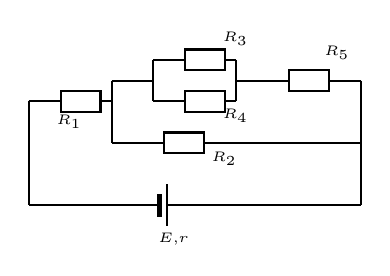
\begin{tikzpicture}[x=0.75pt,y=0.75pt,yscale=-1,xscale=1]
%uncomment if require: \path (0,300); %set diagram left start at 0, and has height of 300

%Shape: Battery [id:dp41038864580231404] 
\draw   (160,130) -- (173.5,130) (176.5,120) -- (176.5,140) (176.5,130) -- (190,130) (172.3,125) -- (173.5,125) -- (173.5,135) -- (172.3,135) -- (172.3,125) -- cycle ;
%Straight Lines [id:da3163365738659809] 
\draw    (190,130) -- (270,130) ;
%Straight Lines [id:da05173675712222314] 
\draw    (110,80) -- (110,130) ;
%Straight Lines [id:da47804297862757794] 
\draw    (110,80) -- (120,80) ;
%Straight Lines [id:da9057643206618209] 
\draw    (150,70) -- (150,100) ;
%Shape: Resistor [id:dp9965546099949054] 
\draw   (125.4,75) -- (144.6,75) -- (144.6,85) -- (125.4,85) -- (125.4,75) -- cycle (120,80) -- (125.4,80) (144.6,80) -- (150,80) ;
%Straight Lines [id:da0755765621865847] 
\draw    (170,60) -- (170,80) ;
%Straight Lines [id:da5506543591062112] 
\draw    (110,130) -- (160,130) ;
%Shape: Resistor [id:dp5943525570087891] 
\draw   (175.4,95) -- (194.6,95) -- (194.6,105) -- (175.4,105) -- (175.4,95) -- cycle (170,100) -- (175.4,100) (194.6,100) -- (200,100) ;
%Straight Lines [id:da20458298027628818] 
\draw    (150,100) -- (170,100) ;
%Straight Lines [id:da4442305975937406] 
\draw    (200,100) -- (270,100) ;
%Straight Lines [id:da35717809113951704] 
\draw    (150,70) -- (170,70) ;
%Straight Lines [id:da3625645367127812] 
\draw    (170,80) -- (180,80) ;
%Shape: Resistor [id:dp27044674641893796] 
\draw   (185.4,75) -- (204.6,75) -- (204.6,85) -- (185.4,85) -- (185.4,75) -- cycle (180,80) -- (185.4,80) (204.6,80) -- (210,80) ;
%Shape: Resistor [id:dp9888935439946336] 
\draw   (185.4,55) -- (204.6,55) -- (204.6,65) -- (185.4,65) -- (185.4,55) -- cycle (180,60) -- (185.4,60) (204.6,60) -- (210,60) ;
%Straight Lines [id:da2570097891204668] 
\draw    (170,60) -- (180,60) ;
%Straight Lines [id:da8597169745318671] 
\draw    (210,60) -- (210,80) ;
%Straight Lines [id:da6968281670670353] 
\draw    (210,70) -- (230,70) ;
%Shape: Resistor [id:dp9106011423679721] 
\draw   (235.4,65) -- (254.6,65) -- (254.6,75) -- (235.4,75) -- (235.4,65) -- cycle (230,70) -- (235.4,70) (254.6,70) -- (260,70) ;
%Straight Lines [id:da7437742845966437] 
\draw    (260,70) -- (270,70) ;
%Straight Lines [id:da46641133055265294] 
\draw    (270,70) -- (270,130) ;

% Text Node
\draw (171,142) node [anchor=north west][inner sep=0.75pt]  [font=\tiny] [align=left] {$\displaystyle \ms E$,$\displaystyle r$};
% Text Node
\draw (122,85) node [anchor=north west][inner sep=0.75pt]  [font=\tiny] [align=left] {$\displaystyle R_{1}$};
% Text Node
\draw (196.6,103) node [anchor=north west][inner sep=0.75pt]  [font=\tiny] [align=left] {$\displaystyle R_{2}$};
% Text Node
\draw (202,45) node [anchor=north west][inner sep=0.75pt]  [font=\tiny] [align=left] {$\displaystyle R_{3}$};
% Text Node
\draw (202,82) node [anchor=north west][inner sep=0.75pt]  [font=\tiny] [align=left] {$\displaystyle R_{4}$};
% Text Node
\draw (251,52) node [anchor=north west][inner sep=0.75pt]  [font=\tiny] [align=left] {$\displaystyle R_{5}$};


\end{tikzpicture}

\end{center}

如图所示,现有一如上较复杂的电路,对于$R_1$和$R_5$,我们\textbf{可以用一个经过电源的回路将这两个电阻相连,若连接此两电阻可以经过电源,我们认为其为等效串联},如下左图所示。

\begin{minipage}[b]{0.45\linewidth}
\begin{center}

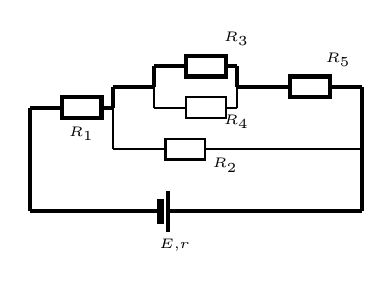
\begin{tikzpicture}[x=0.75pt,y=0.75pt,yscale=-1,xscale=1]
%uncomment if require: \path (0,300); %set diagram left start at 0, and has height of 300

%Shape: Battery [id:dp41038864580231404] 
\draw  [color={rgb, 255:red, 0; green, 0; blue, 0 }  ,draw opacity=1 ][line width=1.5]  (160,130) -- (173.5,130) (176.5,120) -- (176.5,140) (176.5,130) -- (190,130) (172.3,125) -- (173.5,125) -- (173.5,135) -- (172.3,135) -- (172.3,125) -- cycle ;
%Straight Lines [id:da3163365738659809] 
\draw [color={rgb, 255:red, 0; green, 0; blue, 0 }  ,draw opacity=1 ][line width=1.5]    (190,130) -- (270,130) ;
%Straight Lines [id:da05173675712222314] 
\draw [color={rgb, 255:red, 0; green, 0; blue, 0 }  ,draw opacity=1 ][line width=1.5]    (110,80) -- (110,130) ;
%Straight Lines [id:da47804297862757794] 
\draw [color={rgb, 255:red, 0; green, 0; blue, 0 }  ,draw opacity=1 ][line width=1.5]    (110,80) -- (120,80) ;
%Straight Lines [id:da9057643206618209] 
\draw [color={rgb, 255:red, 0; green, 0; blue, 0 }  ,draw opacity=1 ][line width=1.5]    (150,70) -- (150,80) ;
%Shape: Resistor [id:dp9965546099949054] 
\draw  [color={rgb, 255:red, 0; green, 0; blue, 0 }  ,draw opacity=1 ][line width=1.5]  (125.4,75) -- (144.6,75) -- (144.6,85) -- (125.4,85) -- (125.4,75) -- cycle (120,80) -- (125.4,80) (144.6,80) -- (150,80) ;
%Straight Lines [id:da0755765621865847] 
\draw [color={rgb, 255:red, 0; green, 0; blue, 0 }  ,draw opacity=1 ][line width=1.5]    (170,60) -- (170,70) ;
%Straight Lines [id:da5506543591062112] 
\draw [color={rgb, 255:red, 0; green, 0; blue, 0 }  ,draw opacity=1 ][line width=1.5]    (110,130) -- (160,130) ;
%Shape: Resistor [id:dp5943525570087891] 
\draw  [color={rgb, 255:red, 0; green, 0; blue, 0 }  ,draw opacity=1 ] (175.4,95) -- (194.6,95) -- (194.6,105) -- (175.4,105) -- (175.4,95) -- cycle (170,100) -- (175.4,100) (194.6,100) -- (200,100) ;
%Straight Lines [id:da20458298027628818] 
\draw [color={rgb, 255:red, 0; green, 0; blue, 0 }  ,draw opacity=1 ]   (150,100) -- (170,100) ;
%Straight Lines [id:da4442305975937406] 
\draw [color={rgb, 255:red, 0; green, 0; blue, 0 }  ,draw opacity=1 ]   (200,100) -- (270,100) ;
%Straight Lines [id:da35717809113951704] 
\draw [color={rgb, 255:red, 0; green, 0; blue, 0 }  ,draw opacity=1 ][line width=1.5]    (150,70) -- (170,70) ;
%Straight Lines [id:da3625645367127812] 
\draw [color={rgb, 255:red, 0; green, 0; blue, 0 }  ,draw opacity=1 ]   (170,80) -- (180,80) ;
%Shape: Resistor [id:dp27044674641893796] 
\draw  [color={rgb, 255:red, 0; green, 0; blue, 0 }  ,draw opacity=1 ] (185.4,75) -- (204.6,75) -- (204.6,85) -- (185.4,85) -- (185.4,75) -- cycle (180,80) -- (185.4,80) (204.6,80) -- (210,80) ;
%Shape: Resistor [id:dp9888935439946336] 
\draw  [color={rgb, 255:red, 0; green, 0; blue, 0 }  ,draw opacity=1 ][line width=1.5]  (185.4,55) -- (204.6,55) -- (204.6,65) -- (185.4,65) -- (185.4,55) -- cycle (180,60) -- (185.4,60) (204.6,60) -- (210,60) ;
%Straight Lines [id:da2570097891204668] 
\draw [color={rgb, 255:red, 0; green, 0; blue, 0 }  ,draw opacity=1 ][line width=1.5]    (170,60) -- (180,60) ;
%Straight Lines [id:da8597169745318671] 
\draw [color={rgb, 255:red, 0; green, 0; blue, 0 }  ,draw opacity=1 ][line width=1.5]    (210,60) -- (210,70) ;
%Straight Lines [id:da6968281670670353] 
\draw [color={rgb, 255:red, 0; green, 0; blue, 0 }  ,draw opacity=1 ][line width=1.5]    (210,70) -- (230,70) ;
%Shape: Resistor [id:dp9106011423679721] 
\draw  [color={rgb, 255:red, 0; green, 0; blue, 0 }  ,draw opacity=1 ][fill={rgb, 255:red, 255; green, 255; blue, 255 }  ,fill opacity=1 ][line width=1.5]  (235.4,65) -- (254.6,65) -- (254.6,75) -- (235.4,75) -- (235.4,65) -- cycle (230,70) -- (235.4,70) (254.6,70) -- (260,70) ;
%Straight Lines [id:da7437742845966437] 
\draw [color={rgb, 255:red, 0; green, 0; blue, 0 }  ,draw opacity=1 ][line width=1.5]    (260,70) -- (270,70) ;
%Straight Lines [id:da46641133055265294] 
\draw [color={rgb, 255:red, 0; green, 0; blue, 0 }  ,draw opacity=1 ][line width=1.5]    (270,70) -- (270,100) -- (270,130) ;
%Straight Lines [id:da7904655950974608] 
\draw [color={rgb, 255:red, 0; green, 0; blue, 0 }  ,draw opacity=1 ]   (210,70) -- (210,80) ;
%Straight Lines [id:da09045289558828129] 
\draw [color={rgb, 255:red, 0; green, 0; blue, 0 }  ,draw opacity=1 ]   (170,70) -- (170,80) ;
%Straight Lines [id:da8466930385719886] 
\draw [color={rgb, 255:red, 0; green, 0; blue, 0 }  ,draw opacity=1 ]   (150,80) -- (150,100) ;

% Text Node
\draw (171,142) node [anchor=north west][inner sep=0.75pt]  [font=\tiny] [align=left] {$\displaystyle \ms E$,$\displaystyle r$};
% Text Node
\draw (127.4,88) node [anchor=north west][inner sep=0.75pt]  [font=\tiny] [align=left] {$\displaystyle R_{1}$};
% Text Node
\draw (196.6,103) node [anchor=north west][inner sep=0.75pt]  [font=\tiny] [align=left] {$\displaystyle R_{2}$};
% Text Node
\draw (202,42) node [anchor=north west][inner sep=0.75pt]  [font=\tiny] [align=left] {$\displaystyle R_{3}$};
% Text Node
\draw (202,82) node [anchor=north west][inner sep=0.75pt]  [font=\tiny] [align=left] {$\displaystyle R_{4}$};
% Text Node
\draw (251,52) node [anchor=north west][inner sep=0.75pt]  [font=\tiny] [align=left] {$\displaystyle R_{5}$};
\end{tikzpicture}
\end{center}
\end{minipage}
\hfill
\begin{minipage}[b]{0.45\linewidth}
\begin{center}
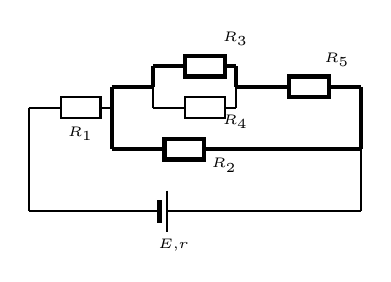
\begin{tikzpicture}[x=0.75pt,y=0.75pt,yscale=-1,xscale=1]
%uncomment if require: \path (0,300); %set diagram left start at 0, and has height of 300

%Shape: Battery [id:dp41038864580231404] 
\draw  [color={rgb, 255:red, 0; green, 0; blue, 0 }  ,draw opacity=1 ][line width=0.75]  (160,130) -- (173.5,130) (176.5,120) -- (176.5,140) (176.5,130) -- (190,130) (172.3,125) -- (173.5,125) -- (173.5,135) -- (172.3,135) -- (172.3,125) -- cycle ;
%Straight Lines [id:da3163365738659809] 
\draw [color={rgb, 255:red, 0; green, 0; blue, 0 }  ,draw opacity=1 ][line width=0.75]    (190,130) -- (270,130) ;
%Straight Lines [id:da05173675712222314] 
\draw [color={rgb, 255:red, 0; green, 0; blue, 0 }  ,draw opacity=1 ][line width=0.75]    (110,80) -- (110,130) ;
%Straight Lines [id:da47804297862757794] 
\draw [color={rgb, 255:red, 0; green, 0; blue, 0 }  ,draw opacity=1 ][line width=0.75]    (110,80) -- (120,80) ;
%Straight Lines [id:da9057643206618209] 
\draw [color={rgb, 255:red, 0; green, 0; blue, 0 }  ,draw opacity=1 ][line width=1.5]    (150,70) -- (150,80) ;
%Shape: Resistor [id:dp9965546099949054] 
\draw  [color={rgb, 255:red, 0; green, 0; blue, 0 }  ,draw opacity=1 ][line width=0.75]  (125.4,75) -- (144.6,75) -- (144.6,85) -- (125.4,85) -- (125.4,75) -- cycle (120,80) -- (125.4,80) (144.6,80) -- (150,80) ;
%Straight Lines [id:da0755765621865847] 
\draw [color={rgb, 255:red, 0; green, 0; blue, 0 }  ,draw opacity=1 ][line width=1.5]    (170,60) -- (170,70) ;
%Straight Lines [id:da5506543591062112] 
\draw [color={rgb, 255:red, 0; green, 0; blue, 0 }  ,draw opacity=1 ][line width=0.75]    (110,130) -- (160,130) ;
%Shape: Resistor [id:dp5943525570087891] 
\draw  [color={rgb, 255:red, 0; green, 0; blue, 0 }  ,draw opacity=1 ][line width=1.5]  (175.4,95) -- (194.6,95) -- (194.6,105) -- (175.4,105) -- (175.4,95) -- cycle (170,100) -- (175.4,100) (194.6,100) -- (200,100) ;
%Straight Lines [id:da20458298027628818] 
\draw [color={rgb, 255:red, 0; green, 0; blue, 0 }  ,draw opacity=1 ][line width=1.5]    (150,100) -- (170,100) ;
%Straight Lines [id:da4442305975937406] 
\draw [color={rgb, 255:red, 0; green, 0; blue, 0 }  ,draw opacity=1 ][line width=1.5]    (200,100) -- (270,100) ;
%Straight Lines [id:da35717809113951704] 
\draw [color={rgb, 255:red, 0; green, 0; blue, 0 }  ,draw opacity=1 ][line width=1.5]    (150,70) -- (170,70) ;
%Straight Lines [id:da3625645367127812] 
\draw [color={rgb, 255:red, 0; green, 0; blue, 0 }  ,draw opacity=1 ][line width=0.75]    (170,80) -- (180,80) ;
%Shape: Resistor [id:dp27044674641893796] 
\draw  [color={rgb, 255:red, 0; green, 0; blue, 0 }  ,draw opacity=1 ][line width=0.75]  (185.4,75) -- (204.6,75) -- (204.6,85) -- (185.4,85) -- (185.4,75) -- cycle (180,80) -- (185.4,80) (204.6,80) -- (210,80) ;
%Shape: Resistor [id:dp9888935439946336] 
\draw  [color={rgb, 255:red, 0; green, 0; blue, 0 }  ,draw opacity=1 ][line width=1.5]  (185.4,55) -- (204.6,55) -- (204.6,65) -- (185.4,65) -- (185.4,55) -- cycle (180,60) -- (185.4,60) (204.6,60) -- (210,60) ;
%Straight Lines [id:da2570097891204668] 
\draw [color={rgb, 255:red, 0; green, 0; blue, 0 }  ,draw opacity=1 ][line width=1.5]    (170,60) -- (180,60) ;
%Straight Lines [id:da8597169745318671] 
\draw [color={rgb, 255:red, 0; green, 0; blue, 0 }  ,draw opacity=1 ][line width=1.5]    (210,60) -- (210,70) ;
%Straight Lines [id:da6968281670670353] 
\draw [color={rgb, 255:red, 0; green, 0; blue, 0 }  ,draw opacity=1 ][line width=1.5]    (210,70) -- (230,70) ;
%Shape: Resistor [id:dp9106011423679721] 
\draw  [color={rgb, 255:red, 0; green, 0; blue, 0 }  ,draw opacity=1 ][fill={rgb, 255:red, 255; green, 255; blue, 255 }  ,fill opacity=1 ][line width=1.5]  (235.4,65) -- (254.6,65) -- (254.6,75) -- (235.4,75) -- (235.4,65) -- cycle (230,70) -- (235.4,70) (254.6,70) -- (260,70) ;
%Straight Lines [id:da7437742845966437] 
\draw [color={rgb, 255:red, 0; green, 0; blue, 0 }  ,draw opacity=1 ][line width=1.5]    (260,70) -- (270,70) ;
%Straight Lines [id:da46641133055265294] 
\draw [color={rgb, 255:red, 0; green, 0; blue, 0 }  ,draw opacity=1 ][line width=1.5]    (270,70) -- (270,100) ;
%Straight Lines [id:da7904655950974608] 
\draw [color={rgb, 255:red, 0; green, 0; blue, 0 }  ,draw opacity=1 ][line width=0.75]    (210,70) -- (210,80) ;
%Straight Lines [id:da09045289558828129] 
\draw [color={rgb, 255:red, 0; green, 0; blue, 0 }  ,draw opacity=1 ][line width=0.75]    (170,70) -- (170,80) ;
%Straight Lines [id:da8466930385719886] 
\draw [color={rgb, 255:red, 0; green, 0; blue, 0 }  ,draw opacity=1 ][line width=1.5]    (150,80) -- (150,100) ;
%Straight Lines [id:da9186238470693386] 
\draw [color={rgb, 255:red, 0; green, 0; blue, 0 }  ,draw opacity=1 ][line width=0.75]    (270,100) -- (270,130) ;

% Text Node
\draw (171,142) node [anchor=north west][inner sep=0.75pt]  [font=\tiny] [align=left] {$\displaystyle \ms E$,$\displaystyle r$};
% Text Node
\draw (127.4,88) node [anchor=north west][inner sep=0.75pt]  [font=\tiny] [align=left] {$\displaystyle R_{1}$};
% Text Node
\draw (196.6,103) node [anchor=north west][inner sep=0.75pt]  [font=\tiny] [align=left] {$\displaystyle R_{2}$};
% Text Node
\draw (202,42) node [anchor=north west][inner sep=0.75pt]  [font=\tiny] [align=left] {$\displaystyle R_{3}$};
% Text Node
\draw (202,82) node [anchor=north west][inner sep=0.75pt]  [font=\tiny] [align=left] {$\displaystyle R_{4}$};
% Text Node
\draw (251,52) node [anchor=north west][inner sep=0.75pt]  [font=\tiny] [align=left] {$\displaystyle R_{5}$};

\end{tikzpicture}
\end{center}
\end{minipage}

对于$R_2$和$R_5$,我们\textbf{不可能用一个经过电源的回路将这两个电阻相连,若连接此两电阻不可以经过电源,我们认为其为等效并联},如上右图所示。\footnote{这里对于如电桥类问题并不适用,因为随着电桥某一桥臂电阻的改变,其经过中间的电阻的电流方向会发生改变,从而改变其等效串并联关系。在此情况下只能根据前文\defiref{gycbl}分情况进行判断。}

如果对于两个电阻,有多种回路将这两个电阻相连,如下图所示,对于$R_1$和$R_5$,可以绘出如下两个回路将两个电阻相连,其中一个经过电源,另一个不经过电源。\textbf{对于这个情况,只要有一个回路经过了电源,那么就可以认为其为广义串联。}

\begin{center}

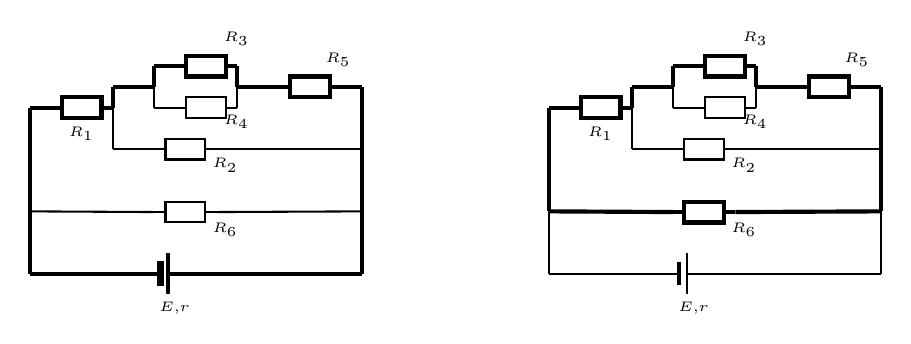
\begin{tikzpicture}[x=0.75pt,y=0.75pt,yscale=-1,xscale=1]
%uncomment if require: \path (0,300); %set diagram left start at 0, and has height of 300

%Shape: Battery [id:dp41038864580231404] 
\draw  [color={rgb, 255:red, 0; green, 0; blue, 0 }  ,draw opacity=1 ][line width=1.5]  (150,200) -- (163.5,200) (166.5,190) -- (166.5,210) (166.5,200) -- (180,200) (162.3,195) -- (163.5,195) -- (163.5,205) -- (162.3,205) -- (162.3,195) -- cycle ;
%Straight Lines [id:da3163365738659809] 
\draw [color={rgb, 255:red, 0; green, 0; blue, 0 }  ,draw opacity=1 ][line width=1.5]    (180,200) -- (260,200) ;
%Straight Lines [id:da05173675712222314] 
\draw [color={rgb, 255:red, 0; green, 0; blue, 0 }  ,draw opacity=1 ][line width=1.5]    (100,120) -- (100,200) ;
%Straight Lines [id:da47804297862757794] 
\draw [color={rgb, 255:red, 0; green, 0; blue, 0 }  ,draw opacity=1 ][line width=1.5]    (100,120) -- (110,120) ;
%Straight Lines [id:da9057643206618209] 
\draw [color={rgb, 255:red, 0; green, 0; blue, 0 }  ,draw opacity=1 ][line width=1.5]    (140,110) -- (140,120) ;
%Shape: Resistor [id:dp9965546099949054] 
\draw  [color={rgb, 255:red, 0; green, 0; blue, 0 }  ,draw opacity=1 ][line width=1.5]  (115.4,115) -- (134.6,115) -- (134.6,125) -- (115.4,125) -- (115.4,115) -- cycle (110,120) -- (115.4,120) (134.6,120) -- (140,120) ;
%Straight Lines [id:da0755765621865847] 
\draw [color={rgb, 255:red, 0; green, 0; blue, 0 }  ,draw opacity=1 ][line width=1.5]    (160,100) -- (160,110) ;
%Straight Lines [id:da5506543591062112] 
\draw [color={rgb, 255:red, 0; green, 0; blue, 0 }  ,draw opacity=1 ][line width=1.5]    (100,200) -- (150,200) ;
%Shape: Resistor [id:dp5943525570087891] 
\draw  [color={rgb, 255:red, 0; green, 0; blue, 0 }  ,draw opacity=1 ][line width=0.75]  (165.4,135) -- (184.6,135) -- (184.6,145) -- (165.4,145) -- (165.4,135) -- cycle (160,140) -- (165.4,140) (184.6,140) -- (190,140) ;
%Straight Lines [id:da20458298027628818] 
\draw [color={rgb, 255:red, 0; green, 0; blue, 0 }  ,draw opacity=1 ][line width=0.75]    (140,140) -- (160,140) ;
%Straight Lines [id:da4442305975937406] 
\draw [color={rgb, 255:red, 0; green, 0; blue, 0 }  ,draw opacity=1 ][line width=0.75]    (190,140) -- (260,140) ;
%Straight Lines [id:da35717809113951704] 
\draw [color={rgb, 255:red, 0; green, 0; blue, 0 }  ,draw opacity=1 ][line width=1.5]    (140,110) -- (160,110) ;
%Straight Lines [id:da3625645367127812] 
\draw [color={rgb, 255:red, 0; green, 0; blue, 0 }  ,draw opacity=1 ][line width=0.75]    (160,120) -- (170,120) ;
%Shape: Resistor [id:dp27044674641893796] 
\draw  [color={rgb, 255:red, 0; green, 0; blue, 0 }  ,draw opacity=1 ][line width=0.75]  (175.4,115) -- (194.6,115) -- (194.6,125) -- (175.4,125) -- (175.4,115) -- cycle (170,120) -- (175.4,120) (194.6,120) -- (200,120) ;
%Shape: Resistor [id:dp9888935439946336] 
\draw  [color={rgb, 255:red, 0; green, 0; blue, 0 }  ,draw opacity=1 ][line width=1.5]  (175.4,95) -- (194.6,95) -- (194.6,105) -- (175.4,105) -- (175.4,95) -- cycle (170,100) -- (175.4,100) (194.6,100) -- (200,100) ;
%Straight Lines [id:da2570097891204668] 
\draw [color={rgb, 255:red, 0; green, 0; blue, 0 }  ,draw opacity=1 ][line width=1.5]    (160,100) -- (170,100) ;
%Straight Lines [id:da8597169745318671] 
\draw [color={rgb, 255:red, 0; green, 0; blue, 0 }  ,draw opacity=1 ][line width=1.5]    (200,100) -- (200,110) ;
%Straight Lines [id:da6968281670670353] 
\draw [color={rgb, 255:red, 0; green, 0; blue, 0 }  ,draw opacity=1 ][line width=1.5]    (200,110) -- (220,110) ;
%Shape: Resistor [id:dp9106011423679721] 
\draw  [color={rgb, 255:red, 0; green, 0; blue, 0 }  ,draw opacity=1 ][fill={rgb, 255:red, 255; green, 255; blue, 255 }  ,fill opacity=1 ][line width=1.5]  (225.4,105) -- (244.6,105) -- (244.6,115) -- (225.4,115) -- (225.4,105) -- cycle (220,110) -- (225.4,110) (244.6,110) -- (250,110) ;
%Straight Lines [id:da7437742845966437] 
\draw [color={rgb, 255:red, 0; green, 0; blue, 0 }  ,draw opacity=1 ][line width=1.5]    (250,110) -- (260,110) ;
%Straight Lines [id:da46641133055265294] 
\draw [color={rgb, 255:red, 0; green, 0; blue, 0 }  ,draw opacity=1 ][line width=1.5]    (260,110) -- (260,140) ;
%Straight Lines [id:da7904655950974608] 
\draw [color={rgb, 255:red, 0; green, 0; blue, 0 }  ,draw opacity=1 ][line width=0.75]    (200,110) -- (200,120) ;
%Straight Lines [id:da09045289558828129] 
\draw [color={rgb, 255:red, 0; green, 0; blue, 0 }  ,draw opacity=1 ][line width=0.75]    (160,110) -- (160,120) ;
%Straight Lines [id:da8466930385719886] 
\draw [color={rgb, 255:red, 0; green, 0; blue, 0 }  ,draw opacity=1 ][line width=0.75]    (140,120) -- (140,140) ;
%Straight Lines [id:da9186238470693386] 
\draw [color={rgb, 255:red, 0; green, 0; blue, 0 }  ,draw opacity=1 ][line width=1.5]    (260,140) -- (260,170) -- (260,200) ;
%Shape: Resistor [id:dp7743010446542762] 
\draw  [color={rgb, 255:red, 0; green, 0; blue, 0 }  ,draw opacity=1 ][line width=0.75]  (165.4,165.33) -- (184.6,165.33) -- (184.6,175.33) -- (165.4,175.33) -- (165.4,165.33) -- cycle (160,170.33) -- (165.4,170.33) (184.6,170.33) -- (190,170.33) ;
%Straight Lines [id:da49531474597430103] 
\draw [color={rgb, 255:red, 0; green, 0; blue, 0 }  ,draw opacity=1 ][line width=0.75]    (100,170) -- (160,170.33) ;
%Straight Lines [id:da295802229690765] 
\draw [color={rgb, 255:red, 0; green, 0; blue, 0 }  ,draw opacity=1 ][line width=0.75]    (190,170.33) -- (260,170) ;
%Shape: Battery [id:dp21438829949628424] 
\draw  [color={rgb, 255:red, 0; green, 0; blue, 0 }  ,draw opacity=1 ][line width=0.75]  (400,200) -- (413.5,200) (416.5,190) -- (416.5,210) (416.5,200) -- (430,200) (412.3,195) -- (413.5,195) -- (413.5,205) -- (412.3,205) -- (412.3,195) -- cycle ;
%Straight Lines [id:da5422220253090375] 
\draw [color={rgb, 255:red, 0; green, 0; blue, 0 }  ,draw opacity=1 ][line width=0.75]    (430,200) -- (510,200) ;
%Straight Lines [id:da3345656290393828] 
\draw [color={rgb, 255:red, 0; green, 0; blue, 0 }  ,draw opacity=1 ][line width=1.5]    (350,120) -- (350,170) ;
%Straight Lines [id:da9218491560734923] 
\draw [color={rgb, 255:red, 0; green, 0; blue, 0 }  ,draw opacity=1 ][line width=1.5]    (350,120) -- (360,120) ;
%Straight Lines [id:da05910857835576011] 
\draw [color={rgb, 255:red, 0; green, 0; blue, 0 }  ,draw opacity=1 ][line width=1.5]    (390,110) -- (390,120) ;
%Shape: Resistor [id:dp5844795040319717] 
\draw  [color={rgb, 255:red, 0; green, 0; blue, 0 }  ,draw opacity=1 ][line width=1.5]  (365.4,115) -- (384.6,115) -- (384.6,125) -- (365.4,125) -- (365.4,115) -- cycle (360,120) -- (365.4,120) (384.6,120) -- (390,120) ;
%Straight Lines [id:da34103379296083935] 
\draw [color={rgb, 255:red, 0; green, 0; blue, 0 }  ,draw opacity=1 ][line width=1.5]    (410,100) -- (410,110) ;
%Straight Lines [id:da1389634467176808] 
\draw [color={rgb, 255:red, 0; green, 0; blue, 0 }  ,draw opacity=1 ][line width=0.75]    (350,200) -- (400,200) ;
%Shape: Resistor [id:dp3486134027487422] 
\draw  [color={rgb, 255:red, 0; green, 0; blue, 0 }  ,draw opacity=1 ][line width=0.75]  (415.4,135) -- (434.6,135) -- (434.6,145) -- (415.4,145) -- (415.4,135) -- cycle (410,140) -- (415.4,140) (434.6,140) -- (440,140) ;
%Straight Lines [id:da35393799851262453] 
\draw [color={rgb, 255:red, 0; green, 0; blue, 0 }  ,draw opacity=1 ][line width=0.75]    (390,140) -- (410,140) ;
%Straight Lines [id:da5235864546499926] 
\draw [color={rgb, 255:red, 0; green, 0; blue, 0 }  ,draw opacity=1 ][line width=0.75]    (440,140) -- (510,140) ;
%Straight Lines [id:da1786703994427281] 
\draw [color={rgb, 255:red, 0; green, 0; blue, 0 }  ,draw opacity=1 ][line width=1.5]    (390,110) -- (410,110) ;
%Straight Lines [id:da2581200495495104] 
\draw [color={rgb, 255:red, 0; green, 0; blue, 0 }  ,draw opacity=1 ][line width=0.75]    (410,120) -- (420,120) ;
%Shape: Resistor [id:dp35308148981638676] 
\draw  [color={rgb, 255:red, 0; green, 0; blue, 0 }  ,draw opacity=1 ][line width=0.75]  (425.4,115) -- (444.6,115) -- (444.6,125) -- (425.4,125) -- (425.4,115) -- cycle (420,120) -- (425.4,120) (444.6,120) -- (450,120) ;
%Shape: Resistor [id:dp11373317493821555] 
\draw  [color={rgb, 255:red, 0; green, 0; blue, 0 }  ,draw opacity=1 ][line width=1.5]  (425.4,95) -- (444.6,95) -- (444.6,105) -- (425.4,105) -- (425.4,95) -- cycle (420,100) -- (425.4,100) (444.6,100) -- (450,100) ;
%Straight Lines [id:da4077457408934002] 
\draw [color={rgb, 255:red, 0; green, 0; blue, 0 }  ,draw opacity=1 ][line width=1.5]    (410,100) -- (420,100) ;
%Straight Lines [id:da2520265830597921] 
\draw [color={rgb, 255:red, 0; green, 0; blue, 0 }  ,draw opacity=1 ][line width=1.5]    (450,100) -- (450,110) ;
%Straight Lines [id:da35239844900214257] 
\draw [color={rgb, 255:red, 0; green, 0; blue, 0 }  ,draw opacity=1 ][line width=1.5]    (450,110) -- (470,110) ;
%Shape: Resistor [id:dp35464885852764816] 
\draw  [color={rgb, 255:red, 0; green, 0; blue, 0 }  ,draw opacity=1 ][fill={rgb, 255:red, 255; green, 255; blue, 255 }  ,fill opacity=1 ][line width=1.5]  (475.4,105) -- (494.6,105) -- (494.6,115) -- (475.4,115) -- (475.4,105) -- cycle (470,110) -- (475.4,110) (494.6,110) -- (500,110) ;
%Straight Lines [id:da014196159024891353] 
\draw [color={rgb, 255:red, 0; green, 0; blue, 0 }  ,draw opacity=1 ][line width=1.5]    (500,110) -- (510,110) ;
%Straight Lines [id:da44802775040766374] 
\draw [color={rgb, 255:red, 0; green, 0; blue, 0 }  ,draw opacity=1 ][line width=1.5]    (510,110) -- (510,140) ;
%Straight Lines [id:da5485925662271229] 
\draw [color={rgb, 255:red, 0; green, 0; blue, 0 }  ,draw opacity=1 ][line width=0.75]    (450,110) -- (450,120) ;
%Straight Lines [id:da026702400335047782] 
\draw [color={rgb, 255:red, 0; green, 0; blue, 0 }  ,draw opacity=1 ][line width=0.75]    (410,110) -- (410,120) ;
%Straight Lines [id:da44512522003518495] 
\draw [color={rgb, 255:red, 0; green, 0; blue, 0 }  ,draw opacity=1 ][line width=0.75]    (390,120) -- (390,140) ;
%Straight Lines [id:da7973757661068601] 
\draw [color={rgb, 255:red, 0; green, 0; blue, 0 }  ,draw opacity=1 ][line width=1.5]    (510,140) -- (510,170) ;
%Shape: Resistor [id:dp9123856221579909] 
\draw  [color={rgb, 255:red, 0; green, 0; blue, 0 }  ,draw opacity=1 ][line width=1.5]  (415.4,165.33) -- (434.6,165.33) -- (434.6,175.33) -- (415.4,175.33) -- (415.4,165.33) -- cycle (410,170.33) -- (415.4,170.33) (434.6,170.33) -- (440,170.33) ;
%Straight Lines [id:da6548936972790516] 
\draw [color={rgb, 255:red, 0; green, 0; blue, 0 }  ,draw opacity=1 ][line width=1.5]    (350,170) -- (410,170.33) ;
%Straight Lines [id:da30508875855489204] 
\draw [color={rgb, 255:red, 0; green, 0; blue, 0 }  ,draw opacity=1 ][line width=1.5]    (440,170.33) -- (510,170) ;
%Straight Lines [id:da2334301925578779] 
\draw [color={rgb, 255:red, 0; green, 0; blue, 0 }  ,draw opacity=1 ][line width=0.75]    (510,170) -- (510,200) ;
%Straight Lines [id:da10288926384067398] 
\draw [color={rgb, 255:red, 0; green, 0; blue, 0 }  ,draw opacity=1 ][line width=0.75]    (350,170) -- (350,200) ;

% Text Node
\draw (161,212) node [anchor=north west][inner sep=0.75pt]  [font=\tiny] [align=left] {$\displaystyle \ms E$,$\displaystyle r$};
% Text Node
\draw (117.4,128) node [anchor=north west][inner sep=0.75pt]  [font=\tiny] [align=left] {$\displaystyle R_{1}$};
% Text Node
\draw (186.6,143) node [anchor=north west][inner sep=0.75pt]  [font=\tiny] [align=left] {$\displaystyle R_{2}$};
% Text Node
\draw (192,82) node [anchor=north west][inner sep=0.75pt]  [font=\tiny] [align=left] {$\displaystyle R_{3}$};
% Text Node
\draw (192,122) node [anchor=north west][inner sep=0.75pt]  [font=\tiny] [align=left] {$\displaystyle R_{4}$};
% Text Node
\draw (241,92) node [anchor=north west][inner sep=0.75pt]  [font=\tiny] [align=left] {$\displaystyle R_{5}$};
% Text Node
\draw (186.6,174) node [anchor=north west][inner sep=0.75pt]  [font=\tiny] [align=left] {$\displaystyle R_{6}$};
% Text Node
\draw (411,212) node [anchor=north west][inner sep=0.75pt]  [font=\tiny] [align=left] {$\displaystyle 
\ms E$,$\displaystyle r$};
% Text Node
\draw (367.4,128) node [anchor=north west][inner sep=0.75pt]  [font=\tiny] [align=left] {$\displaystyle R_{1}$};
% Text Node
\draw (436.6,143) node [anchor=north west][inner sep=0.75pt]  [font=\tiny] [align=left] {$\displaystyle R_{2}$};
% Text Node
\draw (442,82) node [anchor=north west][inner sep=0.75pt]  [font=\tiny] [align=left] {$\displaystyle R_{3}$};
% Text Node
\draw (442,122) node [anchor=north west][inner sep=0.75pt]  [font=\tiny] [align=left] {$\displaystyle R_{4}$};
% Text Node
\draw (491,92) node [anchor=north west][inner sep=0.75pt]  [font=\tiny] [align=left] {$\displaystyle R_{5}$};
% Text Node
\draw (436.6,174) node [anchor=north west][inner sep=0.75pt]  [font=\tiny] [align=left] {$\displaystyle R_{6}$};


\end{tikzpicture}

\end{center}

这里需要注意,串反并同存在使用条件,如下

\begin{mk}{易错提醒}{}
当且仅当\textbf{电源存在内阻}以及\textbf{只有单个电阻变化}时,才可以运用“串反并同”。
\end{mk}

当然,根据前文\theoref{dwndl},可以通过将不存在内阻的理想电压源跟外电路的电阻等效成具有内阻的电源而使用串反并同,具体可见如下例题。

\begin{ep}{2009·广东}{}

\begin{center}

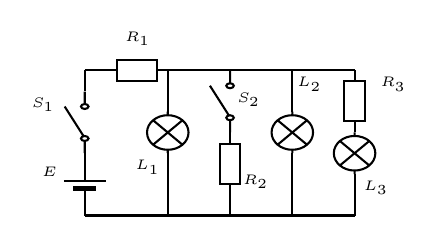
\begin{tikzpicture}[x=0.75pt,y=0.75pt,yscale=-1,xscale=1]
%uncomment if require: \path (0,300); %set diagram left start at 0, and has height of 300

%Shape: Battery [id:dp797984114545808] 
\draw   (100,170) -- (100,156.5) (90,153.5) -- (110,153.5) (100,153.5) -- (100,140) (95,157.7) -- (95,156.5) -- (105,156.5) -- (105,157.7) -- (95,157.7) -- cycle ;
%Shape: Simple Switch [id:dp4334800063265021] 
\draw   (100,140) -- (100,134.07) (100,116.29) -- (100,110.37) (99.39,131.7) -- (90.32,117.48) (100,118.66) .. controls (99,118.66) and (98.18,118.13) .. (98.18,117.48) .. controls (98.18,116.82) and (99,116.29) .. (100,116.29) .. controls (101,116.29) and (101.82,116.82) .. (101.82,117.48) .. controls (101.82,118.13) and (101,118.66) .. (100,118.66) -- cycle (100,134.07) .. controls (99,134.07) and (98.18,133.54) .. (98.18,132.89) .. controls (98.18,132.23) and (99,131.7) .. (100,131.7) .. controls (101,131.7) and (101.82,132.23) .. (101.82,132.89) .. controls (101.82,133.54) and (101,134.07) .. (100,134.07) -- cycle ;
%Shape: Resistor [id:dp901312688402967] 
\draw   (115.4,95) -- (134.6,95) -- (134.6,105) -- (115.4,105) -- (115.4,95) -- cycle (110,100) -- (115.4,100) (134.6,100) -- (140,100) ;
%Straight Lines [id:da2657385353492341] 
\draw    (100,110) -- (100,100) ;
%Straight Lines [id:da5416440059996896] 
\draw    (100,100) -- (110,100) ;
%Shape: Light Bulb [id:dp598022898779403] 
\draw   (140,138.33) .. controls (134.48,138.33) and (130,134.6) .. (130,130) .. controls (130,125.4) and (134.48,121.67) .. (140,121.67) .. controls (145.52,121.67) and (150,125.4) .. (150,130) .. controls (150,134.6) and (145.52,138.33) .. (140,138.33) -- cycle (132.88,135.93) -- (147.12,124.07) (132.88,124.07) -- (147.12,135.93) (140,140) -- (140,138.33) (140,121.67) -- (140,120) ;
%Straight Lines [id:da4277642056179305] 
\draw    (140,100) -- (140,120) ;
%Straight Lines [id:da9223803374157449] 
\draw    (100,170) -- (230,170) ;
%Straight Lines [id:da4800046187933087] 
\draw    (140,140) -- (140,170) ;
%Straight Lines [id:da5325118901733754] 
\draw    (140,100) -- (230,100) ;
%Shape: Light Bulb [id:dp8429011424978414] 
\draw   (200,138.33) .. controls (194.48,138.33) and (190,134.6) .. (190,130) .. controls (190,125.4) and (194.48,121.67) .. (200,121.67) .. controls (205.52,121.67) and (210,125.4) .. (210,130) .. controls (210,134.6) and (205.52,138.33) .. (200,138.33) -- cycle (192.88,135.93) -- (207.12,124.07) (192.88,124.07) -- (207.12,135.93) (200,140) -- (200,138.33) (200,121.67) -- (200,120) ;
%Straight Lines [id:da06826023906061329] 
\draw    (200,100) -- (200,120) ;
%Straight Lines [id:da15676855229008013] 
\draw    (200,140) -- (200,170) ;
%Shape: Simple Switch [id:dp5417474493250272] 
\draw   (170,130) -- (170,124.07) (170,106.29) -- (170,100.37) (169.39,121.7) -- (160.32,107.48) (170,108.66) .. controls (169,108.66) and (168.18,108.13) .. (168.18,107.48) .. controls (168.18,106.82) and (169,106.29) .. (170,106.29) .. controls (171,106.29) and (171.82,106.82) .. (171.82,107.48) .. controls (171.82,108.13) and (171,108.66) .. (170,108.66) -- cycle (170,124.07) .. controls (169,124.07) and (168.18,123.54) .. (168.18,122.89) .. controls (168.18,122.23) and (169,121.7) .. (170,121.7) .. controls (171,121.7) and (171.82,122.23) .. (171.82,122.89) .. controls (171.82,123.54) and (171,124.07) .. (170,124.07) -- cycle ;
%Shape: Resistor [id:dp5887325110380754] 
\draw   (165,154.6) -- (165,135.4) -- (175,135.4) -- (175,154.6) -- (165,154.6) -- cycle (170,160) -- (170,154.6) (170,135.4) -- (170,130) ;
%Straight Lines [id:da997349339495381] 
\draw    (170,160) -- (170,170) ;
%Straight Lines [id:da908902191522615] 
\draw    (230,150) -- (230,170) ;
%Shape: Light Bulb [id:dp15511171823131908] 
\draw   (230,148.33) .. controls (224.48,148.33) and (220,144.6) .. (220,140) .. controls (220,135.4) and (224.48,131.67) .. (230,131.67) .. controls (235.52,131.67) and (240,135.4) .. (240,140) .. controls (240,144.6) and (235.52,148.33) .. (230,148.33) -- cycle (222.88,145.93) -- (237.12,134.07) (222.88,134.07) -- (237.12,145.93) (230,150) -- (230,148.33) (230,131.67) -- (230,130) ;
%Shape: Resistor [id:dp2189689923867002] 
\draw   (225,124.6) -- (225,105.4) -- (235,105.4) -- (235,124.6) -- (225,124.6) -- cycle (230,130) -- (230,124.6) (230,105.4) -- (230,100) ;

% Text Node
\draw (78,145) node [anchor=north west][inner sep=0.75pt]  [font=\tiny] [align=left] {$\displaystyle E$};
% Text Node
\draw (73,112) node [anchor=north west][inner sep=0.75pt]  [font=\tiny] [align=left] {$\displaystyle S_{1}$};
% Text Node
\draw (172,109.29) node [anchor=north west][inner sep=0.75pt]  [font=\tiny] [align=left] {$\displaystyle S_{2}$};
% Text Node
\draw (118,80) node [anchor=north west][inner sep=0.75pt]  [font=\tiny] [align=left] {$\displaystyle R_{1}$};
% Text Node
\draw (174.8,148.8) node [anchor=north west][inner sep=0.75pt]  [font=\tiny] [align=left] {$\displaystyle R_{2}$};
% Text Node
\draw (241,102) node [anchor=north west][inner sep=0.75pt]  [font=\tiny] [align=left] {$\displaystyle R_{3}$};
% Text Node
\draw (123,142) node [anchor=north west][inner sep=0.75pt]  [font=\tiny] [align=left] {$\displaystyle L_{1}$};
% Text Node
\draw (201,102) node [anchor=north west][inner sep=0.75pt]  [font=\tiny] [align=left] {$\displaystyle L_{2}$};
% Text Node
\draw (233,152) node [anchor=north west][inner sep=0.75pt]  [font=\tiny] [align=left] {$\displaystyle L_{3}$};


\end{tikzpicture}

\end{center}

如图所示,电动势为$E$、内阻不计的电源与三个灯泡和三个电阻相接,只合上开关$S_1$,三个灯泡都能正常工作,如果再合上$S_2$,则下列表述正确的是()

\begin{enumerate}[label=(\Alph*)]
  \item 电源输出功率减小
  \item $L_1$上消耗的功率增大
  \item 通过$R_1$上的电流增大
  \item 通过$R_3$上的电流增大
\end{enumerate}

~\\
\textbf{闭合$S_2$,可以认为$S_2$所在支路电阻由无穷大变为$R_2$},电路总电阻$R_{tot}$变小。注意到\textbf{电源内阻不计},故输出功率$P=\frac{\ms E^2}{R_{tot}}$变大($\ms E = E$,下同),A错误。

\textbf{虽然电源内阻不计,但我们可以运用\secref{s_dxy},将电动势$\ms E$与$R_1$等效成一个电动势为$\ms E$,内阻为$R_1$的内阻,从而满足“串反并同”使用条件。}

\begin{center}
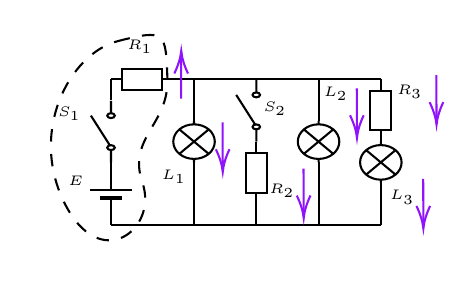
\begin{tikzpicture}[x=0.75pt,y=0.75pt,yscale=-1,xscale=1]
%uncomment if require: \path (0,300); %set diagram left start at 0, and has height of 300

%Shape: Battery [id:dp797984114545808] 
\draw   (100,170) -- (100,156.5) (90,153.5) -- (110,153.5) (100,153.5) -- (100,140) (95,157.7) -- (95,156.5) -- (105,156.5) -- (105,157.7) -- (95,157.7) -- cycle ;
%Shape: Simple Switch [id:dp4334800063265021] 
\draw   (100,140) -- (100,134.07) (100,116.29) -- (100,110.37) (99.39,131.7) -- (90.32,117.48) (100,118.66) .. controls (99,118.66) and (98.18,118.13) .. (98.18,117.48) .. controls (98.18,116.82) and (99,116.29) .. (100,116.29) .. controls (101,116.29) and (101.82,116.82) .. (101.82,117.48) .. controls (101.82,118.13) and (101,118.66) .. (100,118.66) -- cycle (100,134.07) .. controls (99,134.07) and (98.18,133.54) .. (98.18,132.89) .. controls (98.18,132.23) and (99,131.7) .. (100,131.7) .. controls (101,131.7) and (101.82,132.23) .. (101.82,132.89) .. controls (101.82,133.54) and (101,134.07) .. (100,134.07) -- cycle ;
%Shape: Resistor [id:dp901312688402967] 
\draw   (105.4,95) -- (124.6,95) -- (124.6,105) -- (105.4,105) -- (105.4,95) -- cycle (100,100) -- (105.4,100) (124.6,100) -- (130,100) ;
%Straight Lines [id:da2657385353492341] 
\draw    (100,110) -- (100,100) ;
%Straight Lines [id:da5416440059996896] 
\draw    (100,100) ;
%Shape: Light Bulb [id:dp598022898779403] 
\draw   (140,138.33) .. controls (134.48,138.33) and (130,134.6) .. (130,130) .. controls (130,125.4) and (134.48,121.67) .. (140,121.67) .. controls (145.52,121.67) and (150,125.4) .. (150,130) .. controls (150,134.6) and (145.52,138.33) .. (140,138.33) -- cycle (132.88,135.93) -- (147.12,124.07) (132.88,124.07) -- (147.12,135.93) (140,140) -- (140,138.33) (140,121.67) -- (140,120) ;
%Straight Lines [id:da4277642056179305] 
\draw    (140,100) -- (140,120) ;
%Straight Lines [id:da9223803374157449] 
\draw    (100,170) -- (230,170) ;
%Straight Lines [id:da4800046187933087] 
\draw    (140,140) -- (140,170) ;
%Straight Lines [id:da5325118901733754] 
\draw    (130,100) -- (230,100) ;
%Shape: Light Bulb [id:dp8429011424978414] 
\draw   (200,138.33) .. controls (194.48,138.33) and (190,134.6) .. (190,130) .. controls (190,125.4) and (194.48,121.67) .. (200,121.67) .. controls (205.52,121.67) and (210,125.4) .. (210,130) .. controls (210,134.6) and (205.52,138.33) .. (200,138.33) -- cycle (192.88,135.93) -- (207.12,124.07) (192.88,124.07) -- (207.12,135.93) (200,140) -- (200,138.33) (200,121.67) -- (200,120) ;
%Straight Lines [id:da06826023906061329] 
\draw    (200,100) -- (200,120) ;
%Straight Lines [id:da15676855229008013] 
\draw    (200,140) -- (200,170) ;
%Shape: Simple Switch [id:dp5417474493250272] 
\draw   (170,130) -- (170,124.07) (170,106.29) -- (170,100.37) (169.39,121.7) -- (160.32,107.48) (170,108.66) .. controls (169,108.66) and (168.18,108.13) .. (168.18,107.48) .. controls (168.18,106.82) and (169,106.29) .. (170,106.29) .. controls (171,106.29) and (171.82,106.82) .. (171.82,107.48) .. controls (171.82,108.13) and (171,108.66) .. (170,108.66) -- cycle (170,124.07) .. controls (169,124.07) and (168.18,123.54) .. (168.18,122.89) .. controls (168.18,122.23) and (169,121.7) .. (170,121.7) .. controls (171,121.7) and (171.82,122.23) .. (171.82,122.89) .. controls (171.82,123.54) and (171,124.07) .. (170,124.07) -- cycle ;
%Shape: Resistor [id:dp5887325110380754] 
\draw   (165,154.6) -- (165,135.4) -- (175,135.4) -- (175,154.6) -- (165,154.6) -- cycle (170,160) -- (170,154.6) (170,135.4) -- (170,130) ;
%Straight Lines [id:da997349339495381] 
\draw    (170,160) -- (170,170) ;
%Straight Lines [id:da908902191522615] 
\draw    (230,150) -- (230,170) ;
%Shape: Light Bulb [id:dp15511171823131908] 
\draw   (230,148.33) .. controls (224.48,148.33) and (220,144.6) .. (220,140) .. controls (220,135.4) and (224.48,131.67) .. (230,131.67) .. controls (235.52,131.67) and (240,135.4) .. (240,140) .. controls (240,144.6) and (235.52,148.33) .. (230,148.33) -- cycle (222.88,145.93) -- (237.12,134.07) (222.88,134.07) -- (237.12,145.93) (230,150) -- (230,148.33) (230,131.67) -- (230,130) ;
%Shape: Resistor [id:dp2189689923867002] 
\draw   (225,124.6) -- (225,105.4) -- (235,105.4) -- (235,124.6) -- (225,124.6) -- cycle (230,130) -- (230,124.6) (230,105.4) -- (230,100) ;
%Shape: Polygon Curved [id:ds9951042770971332] 
\draw  [dash pattern={on 4.5pt off 4.5pt}] (103.2,81.6) .. controls (126.4,75.6) and (126.37,77.19) .. (127.17,99.59) .. controls (127.97,121.99) and (107.6,128) .. (115.2,150) .. controls (122.8,172) and (94.85,194.15) .. (77.6,159.6) .. controls (60.35,125.05) and (80,87.6) .. (103.2,81.6) -- cycle ;
%Straight Lines [id:da43974811049545215] 
\draw [color={rgb, 255:red, 144; green, 19; blue, 254 }  ,draw opacity=1 ]   (192.75,143) -- (192.83,164.92) ;
\draw [shift={(192.84,166.92)}, rotate = 269.79] [color={rgb, 255:red, 144; green, 19; blue, 254 }  ,draw opacity=1 ][line width=0.75]    (10.93,-3.29) .. controls (6.95,-1.4) and (3.31,-0.3) .. (0,0) .. controls (3.31,0.3) and (6.95,1.4) .. (10.93,3.29)   ;
%Straight Lines [id:da6028004259046089] 
\draw [color={rgb, 255:red, 144; green, 19; blue, 254 }  ,draw opacity=1 ]   (218.41,104.33) -- (218.5,126.25) ;
\draw [shift={(218.5,128.25)}, rotate = 269.79] [color={rgb, 255:red, 144; green, 19; blue, 254 }  ,draw opacity=1 ][line width=0.75]    (10.93,-3.29) .. controls (6.95,-1.4) and (3.31,-0.3) .. (0,0) .. controls (3.31,0.3) and (6.95,1.4) .. (10.93,3.29)   ;
%Straight Lines [id:da18779689260168553] 
\draw [color={rgb, 255:red, 144; green, 19; blue, 254 }  ,draw opacity=1 ]   (250.41,148) -- (250.5,169.92) ;
\draw [shift={(250.5,171.92)}, rotate = 269.79] [color={rgb, 255:red, 144; green, 19; blue, 254 }  ,draw opacity=1 ][line width=0.75]    (10.93,-3.29) .. controls (6.95,-1.4) and (3.31,-0.3) .. (0,0) .. controls (3.31,0.3) and (6.95,1.4) .. (10.93,3.29)   ;
%Straight Lines [id:da47575786229871486] 
\draw [color={rgb, 255:red, 144; green, 19; blue, 254 }  ,draw opacity=1 ]   (256.75,98) -- (256.83,119.92) ;
\draw [shift={(256.84,121.92)}, rotate = 269.79] [color={rgb, 255:red, 144; green, 19; blue, 254 }  ,draw opacity=1 ][line width=0.75]    (10.93,-3.29) .. controls (6.95,-1.4) and (3.31,-0.3) .. (0,0) .. controls (3.31,0.3) and (6.95,1.4) .. (10.93,3.29)   ;
%Straight Lines [id:da9611002858605389] 
\draw [color={rgb, 255:red, 144; green, 19; blue, 254 }  ,draw opacity=1 ]   (153.75,120.67) -- (153.83,142.59) ;
\draw [shift={(153.84,144.59)}, rotate = 269.79] [color={rgb, 255:red, 144; green, 19; blue, 254 }  ,draw opacity=1 ][line width=0.75]    (10.93,-3.29) .. controls (6.95,-1.4) and (3.31,-0.3) .. (0,0) .. controls (3.31,0.3) and (6.95,1.4) .. (10.93,3.29)   ;
%Straight Lines [id:da5346762576536745] 
\draw [color={rgb, 255:red, 144; green, 19; blue, 254 }  ,draw opacity=1 ]   (133.75,109.33) -- (133.83,88.25) ;
\draw [shift={(133.84,86.25)}, rotate = 90.22] [color={rgb, 255:red, 144; green, 19; blue, 254 }  ,draw opacity=1 ][line width=0.75]    (10.93,-3.29) .. controls (6.95,-1.4) and (3.31,-0.3) .. (0,0) .. controls (3.31,0.3) and (6.95,1.4) .. (10.93,3.29)   ;

% Text Node
\draw (78,145) node [anchor=north west][inner sep=0.75pt]  [font=\tiny] [align=left] {$\displaystyle E$};
% Text Node
\draw (73,112) node [anchor=north west][inner sep=0.75pt]  [font=\tiny] [align=left] {$\displaystyle S_{1}$};
% Text Node
\draw (172,109.29) node [anchor=north west][inner sep=0.75pt]  [font=\tiny] [align=left] {$\displaystyle S_{2}$};
% Text Node
\draw (106.33,79.67) node [anchor=north west][inner sep=0.75pt]  [font=\tiny] [align=left] {$\displaystyle R_{1}$};
% Text Node
\draw (174.8,148.8) node [anchor=north west][inner sep=0.75pt]  [font=\tiny] [align=left] {$\displaystyle R_{2}$};
% Text Node
\draw (236.33,101) node [anchor=north west][inner sep=0.75pt]  [font=\tiny] [align=left] {$\displaystyle R_{3}$};
% Text Node
\draw (123,142) node [anchor=north west][inner sep=0.75pt]  [font=\tiny] [align=left] {$\displaystyle L_{1}$};
% Text Node
\draw (201,102) node [anchor=north west][inner sep=0.75pt]  [font=\tiny] [align=left] {$\displaystyle L_{2}$};
% Text Node
\draw (233,152) node [anchor=north west][inner sep=0.75pt]  [font=\tiny] [align=left] {$\displaystyle L_{3}$};

\end{tikzpicture}
\end{center}

如图,当$S_2$所在支路电阻减小时,其各部分电压、电流变化根据“串反并同”如图所示。因此B、D错误,C正确。综上所述,答案为C。

\end{ep}

涉及到与电容器有关的电路问题时,我们可以把电容器当成一个理想的电压表,从而使用“串反并同”。\textbf{但需注意,电容器本质上是断路(在直流电路中),因此跟电容器处在同一支路中串联的电阻改变并不影响电容器两端电压!}具体可见如下例题。

\begin{ep}{2014·天津}{}

\begin{center}
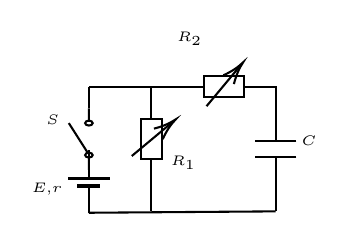
\begin{tikzpicture}[x=0.75pt,y=0.75pt,yscale=-1,xscale=1]
%uncomment if require: \path (0,300); %set diagram left start at 0, and has height of 300

%Shape: Battery [id:dp9725213714143768] 
\draw   (120,180.67) -- (120,167.17) (110,164.17) -- (130,164.17) (120,164.17) -- (120,150.67) (115,168.37) -- (115,167.17) -- (125,167.17) -- (125,168.37) -- (115,168.37) -- cycle ;
%Shape: Simple Switch [id:dp9513460496272634] 
\draw   (120,160) -- (120,154.07) (120,136.29) -- (120,130.37) (119.39,151.7) -- (110.32,137.48) (120,138.66) .. controls (119,138.66) and (118.18,138.13) .. (118.18,137.48) .. controls (118.18,136.82) and (119,136.29) .. (120,136.29) .. controls (121,136.29) and (121.82,136.82) .. (121.82,137.48) .. controls (121.82,138.13) and (121,138.66) .. (120,138.66) -- cycle (120,154.07) .. controls (119,154.07) and (118.18,153.54) .. (118.18,152.89) .. controls (118.18,152.23) and (119,151.7) .. (120,151.7) .. controls (121,151.7) and (121.82,152.23) .. (121.82,152.89) .. controls (121.82,153.54) and (121,154.07) .. (120,154.07) -- cycle ;
%Straight Lines [id:da13406352029154833] 
\draw    (120,130) -- (120,120) ;
%Shape: Resistor [id:dp7782080231234687] 
\draw   (145,154.6) -- (145,135.4) -- (155,135.4) -- (155,154.6) -- (145,154.6) -- cycle (150,160) -- (150,154.6) (150,135.4) -- (150,130) ;
%Straight Lines [id:da13059673417265527] 
\draw    (140.67,153.33) -- (160.3,136.96) ;
\draw [shift={(161.84,135.67)}, rotate = 140.17] [color={rgb, 255:red, 0; green, 0; blue, 0 }  ][line width=0.75]    (10.93,-3.29) .. controls (6.95,-1.4) and (3.31,-0.3) .. (0,0) .. controls (3.31,0.3) and (6.95,1.4) .. (10.93,3.29)   ;

%Straight Lines [id:da15333654490325355] 
\draw    (120,120) -- (170,120) ;
%Straight Lines [id:da8531691012035736] 
\draw    (150,130) -- (150,120) ;
%Straight Lines [id:da4440724028211367] 
\draw    (150,180) -- (150,160) ;
%Shape: Resistor [id:dp2809007889817905] 
\draw   (175.4,125) -- (194.6,125) -- (194.6,115) -- (175.4,115) -- (175.4,125) -- cycle (170,120) -- (175.4,120) (194.6,120) -- (200,120) ;
%Straight Lines [id:da8392657712741902] 
\draw    (176.67,129.33) -- (193.04,109.7) ;
\draw [shift={(194.33,108.16)}, rotate = 129.83] [color={rgb, 255:red, 0; green, 0; blue, 0 }  ][line width=0.75]    (10.93,-3.29) .. controls (6.95,-1.4) and (3.31,-0.3) .. (0,0) .. controls (3.31,0.3) and (6.95,1.4) .. (10.93,3.29)   ;

%Straight Lines [id:da5062655598048114] 
\draw    (200,120) -- (210,120) -- (210,140) ;
%Shape: Contact [id:dp3034505709269577] 
\draw   (210,140) -- (210,146) (210,160) -- (210,154) (220,146) -- (200,146) (220,154) -- (200,154) ;
%Straight Lines [id:da6904084679904827] 
\draw    (210,180) -- (210,160) ;
%Straight Lines [id:da5835108292810021] 
\draw    (120,180.67) -- (210,180) ;

% Text Node
\draw (91,165) node [anchor=north west][inner sep=0.75pt]  [font=\tiny] [align=left] {$\displaystyle E$,$\displaystyle r$};
% Text Node
\draw (98,132) node [anchor=north west][inner sep=0.75pt]  [font=\tiny] [align=left] {$\displaystyle S$};
% Text Node
\draw (158,152) node [anchor=north west][inner sep=0.75pt]  [font=\tiny] [align=left] {$\displaystyle R_{1}$};
% Text Node
\draw (161,92) node [anchor=north west][inner sep=0.75pt]  [font=\tiny] [align=left] {$\displaystyle R_{2}$};
% Text Node
\draw (221,142) node [anchor=north west][inner sep=0.75pt]  [font=\tiny] [align=left] {$\displaystyle C$};


\end{tikzpicture}

\end{center}

如图所示,电路中$R_1$、$R_2$均为可变电阻,电源内阻不能忽
略。平行板电容器$C$的极板水平放置。闭合电键$S$,电路达到稳定时,带电油滴悬浮在两板之间静止不动。如果仅改变下列某一个条件,油滴仍能静止不动的是()

(A) 增大$R_1$的阻值 \quad (B) 增大$R_2$的阻值 \quad (C) 增大两板间的距离 \quad (D) 断开电键$S$

~\\
电阻$R_1$与电容$C$等效并联,增大$R_1$,则$C$两端电压增大,无法保持静止不动,选项A错误。

电阻$R_2$与电容$C$在同一支路上串联,故$R_2$的变化不影响电容$C$两端电压,选项B正确。

增大两板间距离,两板间电压不变,增大距离,电场减弱,无法保持静止不动,选项C错误。

断开$S$,电容两端形成回路放电,无法保持静止不动,选项D错误。综上所述,答案为B。
\end{ep}

这里需要注意,对于分压接法的滑动电阻器,分析滑动电阻器的移动时\textbf{不可直接使用“串反并同”},我们可以将滑动变阻器分成两部分,其中一部分与子电路并联,另一部分与前面并联的部分串联,当移动滑动变阻器时,其并联的电阻跟串联的电阻均发生了变化,\textbf{存在多个电阻变化,违反了“串反并同”的适用条件},故不可直接使用“串反并同”。但我们可以借助\secref{dwndl}对子电路进行分析,从而把两个回路建立联系,绕过滑动变阻器进行分析。

当然,更方便的方法是\textbf{将滑动变阻器及其整个子电路等效成一个电阻,从而使用“串反并同”。我们可以把滑动变阻器分成串联部分和并联部分,若有且只有滑动变阻器发生了变化,则滑动变阻器以及整个子电路电阻变化跟串联电阻相同。}

具体操作见下面例题。

\begin{ep}{自编题}{}
\begin{center}
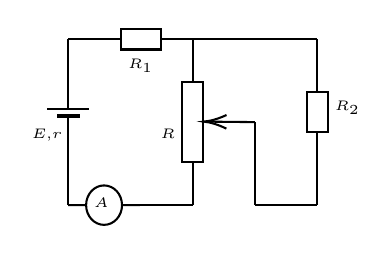
\begin{tikzpicture}[x=0.75pt,y=0.75pt,yscale=-1,xscale=1]
%uncomment if require: \path (0,300); %set diagram left start at 0, and has height of 300

%Straight Lines [id:da9223803374157449] 
\draw    (370,160) -- (430,160) ;
%Straight Lines [id:da4800046187933087] 
\draw    (400,200) -- (400,240) ;
%Straight Lines [id:da15676855229008013] 
\draw    (370,160) -- (370,170) ;
%Shape: Resistor [id:dp5887325110380754] 
\draw   (365,219.2) -- (365,180.8) -- (375,180.8) -- (375,219.2) -- (365,219.2) -- cycle (370,230) -- (370,219.2) (370,180.8) -- (370,170) ;
%Shape: Resistor [id:dp2189689923867002] 
\draw   (425,204.6) -- (425,185.4) -- (435,185.4) -- (435,204.6) -- (425,204.6) -- cycle (430,210) -- (430,204.6) (430,185.4) -- (430,180) ;
%Shape: Battery [id:dp11572428456821915] 
\draw   (310,210) -- (310,196.5) (300,193.5) -- (320,193.5) (310,193.5) -- (310,180) (305,197.7) -- (305,196.5) -- (315,196.5) -- (315,197.7) -- (305,197.7) -- cycle ;
%Straight Lines [id:da5053925872800769] 
\draw    (310,160) -- (310,180) ;
%Shape: Resistor [id:dp8634794872930143] 
\draw   (335.4,155) -- (354.6,155) -- (354.6,165) -- (335.4,165) -- (335.4,155) -- cycle (330,160) -- (335.4,160) (354.6,160) -- (360,160) ;
%Straight Lines [id:da4775642533714568] 
\draw    (310,160) -- (330,160) ;
%Straight Lines [id:da3350904693838317] 
\draw    (360,160) -- (370,160) ;
%Straight Lines [id:da025516599512321214] 
\draw    (310,210) -- (310,240) ;
%Straight Lines [id:da7872440703735311] 
\draw    (370,230) -- (370,240) ;
%Straight Lines [id:da7147480438171852] 
\draw    (400,200) -- (377.34,199.77) ;
\draw [shift={(375.34,199.75)}, rotate = 0.57] [color={rgb, 255:red, 0; green, 0; blue, 0 }  ][line width=0.75]    (10.93,-3.29) .. controls (6.95,-1.4) and (3.31,-0.3) .. (0,0) .. controls (3.31,0.3) and (6.95,1.4) .. (10.93,3.29)   ;
%Shape: Output [id:dp20535874065942084] 
\draw   (318.65,240) .. controls (318.65,234.75) and (322.52,230.5) .. (327.3,230.5) .. controls (332.08,230.5) and (335.95,234.75) .. (335.95,240) .. controls (335.95,245.25) and (332.08,249.5) .. (327.3,249.5) .. controls (322.52,249.5) and (318.65,245.25) .. (318.65,240) -- cycle (310,240) -- (318.65,240) (344.6,240) -- (335.95,240) ;
%Straight Lines [id:da8691520573396538] 
\draw    (340,240) -- (370,240) ;
%Straight Lines [id:da90607602119505] 
\draw    (430,160) -- (430,180) ;
%Straight Lines [id:da522190466993206] 
\draw    (430,210) -- (430,240) ;
%Straight Lines [id:da22747916883790165] 
\draw    (400,240) -- (430,240) ;

% Text Node
\draw (291,202) node [anchor=north west][inner sep=0.75pt]  [font=\tiny] [align=left] {$\displaystyle \ms E$,$\displaystyle r$};
% Text Node
\draw (337.4,168) node [anchor=north west][inner sep=0.75pt]  [font=\tiny] [align=left] {$\displaystyle R_{1}$};
% Text Node
\draw (437,188.4) node [anchor=north west][inner sep=0.75pt]  [font=\tiny] [align=left] {$\displaystyle R_{2}$};
% Text Node
\draw (321,235) node [anchor=north west][inner sep=0.75pt]  [font=\tiny] [align=left] {$\displaystyle A$};
% Text Node
\draw (353,201.67) node [anchor=north west][inner sep=0.75pt]  [font=\tiny] [align=left] {$\displaystyle R$};


\end{tikzpicture}

\end{center}
如图所示电路,内阻不可忽略。现将滑动变阻器$R$的滑片下移,试分析$R_1$、$R_2$两端电压以及电流表$A$的示数$I_A$变化。

~\\
滑片下移,$R$分出的电压更大,即对于子电路而言,电阻$R_2$两端电压增加,电流增加。故通过滑动变阻器$R$的电流增加,滑动变阻器以及子电路等效的电阻减小。由串反并同知$R_1$两端电压增大,电流表$A$示数变大。

当然,由于只有滑动变阻器发生了改变,滑片下移,$R$分出的电压更大,即对于子电路而言,电阻$R_2$两端电压增加,电流增加。滑片下移,其串联部分电阻减小,滑动变阻器以及子电路电阻减小,由串反并同知$R_1$两端电压增大,电流表$A$示数变大。

\end{ep}

\section{变压器等效}

对于变压器问题,一般的方法是对变压器两端列电压方程,再在两个回路中列电学方程,联立求解,这种方法一般会涉及到较多方程的联立,对于选择题等分析判断并不方便,并且有时也不利于运用上文的“串反并同”(见\secref{s_cfbt})。因此,可以通过变压器等效,将其中一个回路等效到另一个回路,从而将一个涉及变压器的双回路问题简化为单回路问题,从而便于运用“串反并同”,简化分析过程,加快计算。

\begin{mk}{符号约定}{}
对于本章节,以下标$L$代表左边的回路的物理量,下标$R$代表右边的回路的物理量。推导出的结论均把下标为$L$的物理量放等号左边,下标为$R$的物理量放右边,这样记忆时只需记忆是正比还是反比即可,更方便。

在下文中,我们将电动势所在的回路上的线圈称为“主线圈”,其回路为“主线圈所在回路”。反之将另一个回路上的线圈称为“从线圈”,其所在回路为“从线圈所在回路”。
\end{mk}

\subsection{变压器电流关系}

对于理想变压器,我们有如下关系

$$\frac{U_L}{n_L} = \frac{U_R}{n_R}, \quad P_L = U_L I_L = U_R I_R = P_R$$

两式相除,得

\begin{equation}
\label{byqdx_eq3}
\boxed{n_L I_L = n_R I_R}
\end{equation}

\begin{center}

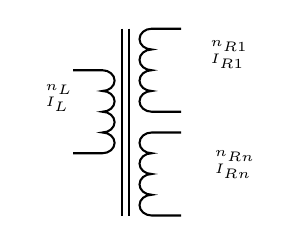
\begin{tikzpicture}[x=0.75pt,y=0.75pt,yscale=-1,xscale=1]
%uncomment if require: \path (0,300); %set diagram left start at 0, and has height of 300

%Shape: Inductor [id:dp27353243461904087] 
\draw   (174.75,120) -- (188.87,120) .. controls (192.11,120) and (194.75,122.24) .. (194.75,125) .. controls (194.75,127.76) and (192.11,130) .. (188.87,130) .. controls (192.11,130) and (194.75,132.24) .. (194.75,135) .. controls (194.75,137.76) and (192.11,140) .. (188.87,140) .. controls (192.11,140) and (194.75,142.24) .. (194.75,145) .. controls (194.75,147.76) and (192.11,150) .. (188.87,150) .. controls (192.11,150) and (194.75,152.24) .. (194.75,155) .. controls (194.75,157.76) and (192.11,160) .. (188.87,160) -- (174.75,160) ;
%Shape: Inductor [id:dp5366739264171354] 
\draw   (226.75,140) -- (212.63,140) .. controls (209.39,140) and (206.75,137.76) .. (206.75,135) .. controls (206.75,132.24) and (209.39,130) .. (212.63,130) .. controls (209.39,130) and (206.75,127.76) .. (206.75,125) .. controls (206.75,122.24) and (209.39,120) .. (212.63,120) .. controls (209.39,120) and (206.75,117.76) .. (206.75,115) .. controls (206.75,112.24) and (209.39,110) .. (212.63,110) .. controls (209.39,110) and (206.75,107.76) .. (206.75,105) .. controls (206.75,102.24) and (209.39,100) .. (212.63,100) -- (226.75,100) ;
%Shape: Inductor [id:dp6707227410735883] 
\draw   (226.75,190) -- (212.63,190) .. controls (209.39,190) and (206.75,187.76) .. (206.75,185) .. controls (206.75,182.24) and (209.39,180) .. (212.63,180) .. controls (209.39,180) and (206.75,177.76) .. (206.75,175) .. controls (206.75,172.24) and (209.39,170) .. (212.63,170) .. controls (209.39,170) and (206.75,167.76) .. (206.75,165) .. controls (206.75,162.24) and (209.39,160) .. (212.63,160) .. controls (209.39,160) and (206.75,157.76) .. (206.75,155) .. controls (206.75,152.24) and (209.39,150) .. (212.63,150) -- (226.75,150) ;
%Straight Lines [id:da43269268551005813] 
\draw    (201.5,100) -- (201.5,190)(198.5,100) -- (198.5,190) ;

% Text Node
\draw (153.37,122.45) node [anchor=north west][inner sep=0.75pt]  [font=\tiny] [align=left] {$\displaystyle  \begin{array}{{>{\displaystyle}l}}
n_{L}\\
I_{L}
\end{array}$};
% Text Node
\draw (232.87,101.7) node [anchor=north west][inner sep=0.75pt]  [font=\tiny] [align=left] {$\displaystyle  \begin{array}{{>{\displaystyle}l}}
n_{R1}\\
I_{R1}
\end{array}$};
% Text Node
\draw (234.87,154.7) node [anchor=north west][inner sep=0.75pt]  [font=\tiny] [align=left] {$\displaystyle  \begin{array}{{>{\displaystyle}l}}
n_{Rn}\\
I_{Rn}
\end{array}$};


\end{tikzpicture}

\end{center}

同理,若存在多个副线圈(如上图),以下标$R1,R2,\cdots,Rn$表示右侧不同副线圈物理量,则

\begin{subequations}
\begin{align}
\label{byqdx_eq1}
\frac{U_L}{n_L} = \frac{U_{R1}}{n_{R1}} = & \cdots = \frac{U_{Rn}}{I_{Rn}} \\
\label{byqdx_eq2}
P_L = U_L I_L = U_{R1} I_{R1} + & \cdots + U_{Rn} I_{Rn} = \sum U_{Ri} I_{Ri}= \sum P_{Ri}
\end{align}
\end{subequations}

用式\eqref{byqdx_eq1}带入式\eqref{byqdx_eq2},化简得

\begin{equation}
\label{byqdx_eq4}
\boxed{n_L I_L = n_{R1} I_{R1} + \cdots + n_{Rn} + I_{Rn} = \sum n_{Ri} I_{Ri}}
\end{equation}

式\eqref{byqdx_eq3}、式\eqref{byqdx_eq4}即为变压器电流关系。

\subsection{变压器等效电阻}

将变压器电压关系$\frac{U_L}{n_L} = \frac{U_R}{n_R}$与电流关系(式\eqref{byqdx_eq3})相除,可得

\begin{equation}
\label{byqdx_eq5}
\boxed{\frac{n_{L}^2}{R_L}=\frac{n_{R}^2}{R_R}}
\end{equation}

同理,对于多个副线圈的情况,可得

\begin{equation}
\label{byqdx_eq6}
\boxed{\frac{n_{L}^2}{R_L} =\frac{n_{R1}^2}{R_{R1}} + \cdots + \frac{n_{Rn}^2}{R_{Rn}} = \sum \frac{n_{Ri}^2}{R_{Ri}}}
\end{equation}

式\eqref{byqdx_eq5}、式\eqref{byqdx_eq6}即为变压器电阻等效公式。

\begin{center}
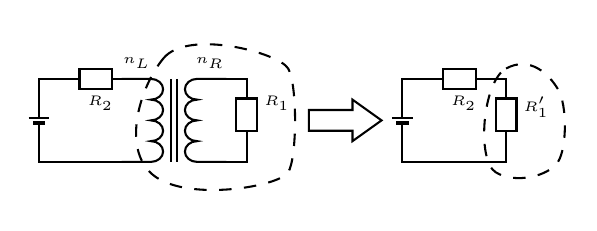
\begin{tikzpicture}[x=0.75pt,y=0.75pt,yscale=-1,xscale=1]
%uncomment if require: \path (0,300); %set diagram left start at 0, and has height of 300

%Shape: Inductor [id:dp27353243461904087] 
\draw   (174.75,120) -- (188.87,120) .. controls (192.11,120) and (194.75,122.24) .. (194.75,125) .. controls (194.75,127.76) and (192.11,130) .. (188.87,130) .. controls (192.11,130) and (194.75,132.24) .. (194.75,135) .. controls (194.75,137.76) and (192.11,140) .. (188.87,140) .. controls (192.11,140) and (194.75,142.24) .. (194.75,145) .. controls (194.75,147.76) and (192.11,150) .. (188.87,150) .. controls (192.11,150) and (194.75,152.24) .. (194.75,155) .. controls (194.75,157.76) and (192.11,160) .. (188.87,160) -- (174.75,160) ;
%Shape: Inductor [id:dp5366739264171354] 
\draw   (225.25,160) -- (211.13,160) .. controls (207.89,160) and (205.25,157.76) .. (205.25,155) .. controls (205.25,152.24) and (207.89,150) .. (211.13,150) .. controls (207.89,150) and (205.25,147.76) .. (205.25,145) .. controls (205.25,142.24) and (207.89,140) .. (211.13,140) .. controls (207.89,140) and (205.25,137.76) .. (205.25,135) .. controls (205.25,132.24) and (207.89,130) .. (211.13,130) .. controls (207.89,130) and (205.25,127.76) .. (205.25,125) .. controls (205.25,122.24) and (207.89,120) .. (211.13,120) -- (225.25,120) ;
%Straight Lines [id:da43269268551005813] 
\draw    (201.5,120) -- (201.5,160)(198.5,120) -- (198.5,160) ;
%Shape: Resistor [id:dp17898965616862061] 
\draw   (154.46,115.28) -- (170.3,115.28) -- (170.3,124.72) -- (154.46,124.72) -- (154.46,115.28) -- cycle (150,120) -- (154.46,120) (170.3,120) -- (174.75,120) ;
%Shape: Resistor [id:dp1038795254331022] 
\draw   (240,129.46) -- (240,145.29) -- (230,145.29) -- (230,129.46) -- (240,129.46) -- cycle (235,125) -- (235,129.46) (235,145.29) -- (235,149.75) ;
%Straight Lines [id:da6753753426347646] 
\draw    (225,120) -- (235,120) -- (235,125) ;
%Straight Lines [id:da7303120384870547] 
\draw    (225.25,160) -- (235,160) -- (235,149.75) ;
%Straight Lines [id:da4345130729061619] 
\draw    (150,120) -- (140,120) ;
%Shape: Battery [id:dp8246420688304279] 
\draw   (135,150) -- (135,140.94) (130,138.93) -- (140,138.93) (135,138.93) -- (135,129.87) (132.5,141.75) -- (132.5,140.94) -- (137.5,140.94) -- (137.5,141.75) -- (132.5,141.75) -- cycle ;
%Straight Lines [id:da43936866820960474] 
\draw    (135,150) -- (135,160) -- (174.75,160) ;
%Straight Lines [id:da690920244145504] 
\draw    (135,130) -- (135,120) -- (140,120) ;
%Left Arrow [id:dp8411203729282917] 
\draw   (300,140) -- (286,150) -- (286,145) -- (265,145) -- (265,135) -- (286,135) -- (286,130) -- cycle ;
%Shape: Polygon Curved [id:ds39327187302490896] 
\draw  [dash pattern={on 4.5pt off 4.5pt}] (195,110) .. controls (206.88,95.83) and (250.5,107.42) .. (255,115) .. controls (259.5,122.58) and (259.37,158.17) .. (255,165) .. controls (250.63,171.83) and (208.13,179.08) .. (191.12,167.2) .. controls (174.12,155.33) and (183.12,124.17) .. (195,110) -- cycle ;
%Shape: Resistor [id:dp3727321464267963] 
\draw   (329.46,115.28) -- (345.3,115.28) -- (345.3,124.72) -- (329.46,124.72) -- (329.46,115.28) -- cycle (325,120) -- (329.46,120) (345.3,120) -- (349.75,120) ;
%Straight Lines [id:da3449293231145629] 
\draw    (325,120) -- (315,120) ;
%Shape: Battery [id:dp28757432788629966] 
\draw   (310,150) -- (310,140.94) (305,138.93) -- (315,138.93) (310,138.93) -- (310,129.87) (307.5,141.75) -- (307.5,140.94) -- (312.5,140.94) -- (312.5,141.75) -- (307.5,141.75) -- cycle ;
%Straight Lines [id:da07750105951735708] 
\draw    (310,150) -- (310,160) -- (349.75,160) ;
%Straight Lines [id:da012940209870557107] 
\draw    (310,130) -- (310,120) -- (315,120) ;
%Shape: Resistor [id:dp3053611810905341] 
\draw   (365,129.45) -- (365,145.3) -- (355,145.3) -- (355,129.45) -- (365,129.45) -- cycle (360,125) -- (360,129.45) (360,145.3) -- (360,149.75) ;
%Straight Lines [id:da2926170106984707] 
\draw    (349.75,120) -- (360,120) -- (360,125) ;
%Straight Lines [id:da6676712847117272] 
\draw    (349.75,160) -- (360,160) -- (360,149.75) ;
%Shape: Polygon Curved [id:ds5017644089146096] 
\draw  [dash pattern={on 4.5pt off 4.5pt}] (360,115) .. controls (371.38,108.83) and (380.5,117.42) .. (385,125) .. controls (389.5,132.58) and (389.37,153.17) .. (385,160) .. controls (380.63,166.83) and (364.38,170.83) .. (355,165) .. controls (345.62,159.17) and (348.62,121.17) .. (360,115) -- cycle ;

% Text Node
\draw (174.12,108.45) node [anchor=north west][inner sep=0.75pt]  [font=\tiny] [align=left] {$\displaystyle n_{L}$};
% Text Node
\draw (209.12,108.2) node [anchor=north west][inner sep=0.75pt]  [font=\tiny] [align=left] {$\displaystyle n_{R}$};
% Text Node
\draw (242,127) node [anchor=north west][inner sep=0.75pt]  [font=\tiny] [align=left] {$\displaystyle R_{1}$};
% Text Node
\draw (157,127) node [anchor=north west][inner sep=0.75pt]  [font=\tiny] [align=left] {$\displaystyle R_{2}$};
% Text Node
\draw (332,127) node [anchor=north west][inner sep=0.75pt]  [font=\tiny] [align=left] {$\displaystyle R_{2}$};
% Text Node
\draw (367,127) node [anchor=north west][inner sep=0.75pt]  [font=\tiny] [align=left] {$\displaystyle R_{1}^{\prime }$};


\end{tikzpicture}

\end{center}

对于上面的公式的应用需要解释说明,如图,若想将左图电路等效成右图电路,\textbf{那么我们要将左图电路中右边的回路等效到左边的回路,从右向左等效,即用右侧物理量解出左侧等效的物理量},由式\eqref{byqdx_eq5}可知

$$R_1^{\prime} = R_L = \frac{n_L^2}{n_R^2} R_R = \frac{n_L^2}{n_R^2} R_1$$

\begin{mk}{思考}{}
对于存在多个副线圈的情况,有变压器电压关系、变压器电流关系以及变压器等效电阻公式

$$\frac{U_L}{n_L} = \frac{U_{R1}}{n_{R1}} = \cdots = \frac{U_{Rn}}{n_{Rn}}$$
$$n_L I_L = n_{R1} I_{R1} + \cdots + n_{Rn} I_{Rn} = \sum n_{Ri} I_{Ri}$$
$$\frac{n_{L}^2}{R_L} =\frac{n_{R1}^2}{R_{R1}} + \cdots + \frac{n_{Rn}^2}{R_{Rn}} = \sum \frac{n_{Ri}^2}{R_{Ri}}$$

此形式与并联电路下电压、电路、等效电阻公式相类似

$$U_L = U_{R1} = \cdots = U_{Rn}$$
$$I_L = I_{R1} + \cdots + I_{Rn} = \sum I_{Ri}$$
$$\frac{1}{R_L} = \frac{1}{R_{R1}} + \cdots + \frac{1}{R_{Rn}} = \sum \frac{1}{R_{Ri}}$$

思考两者之间在物理上有什么相似性
~\\

对于理想变压器,忽略磁损,我们可以注意到,穿过每一个线圈的磁通量相同,其变化率也相同,而感应电动势正比于线圈匝数和磁通量变化率,类似于并联电路下不同支路两端电压相同,只是多了一个线圈匝数项而已。因此两者在公式形式上相似,在物理情形上也具有一定相似性。
\end{mk}

\subsection{变压器等效电源}

\begin{center}

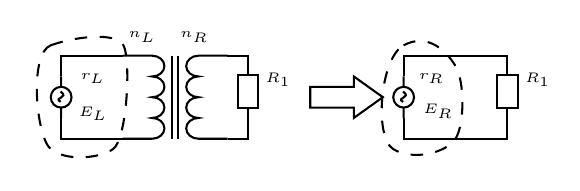
\begin{tikzpicture}[x=0.75pt,y=0.75pt,yscale=-1,xscale=1]
%uncomment if require: \path (0,300); %set diagram left start at 0, and has height of 300

%Shape: Inductor [id:dp27353243461904087] 
\draw   (174.75,120) -- (188.87,120) .. controls (192.11,120) and (194.75,122.24) .. (194.75,125) .. controls (194.75,127.76) and (192.11,130) .. (188.87,130) .. controls (192.11,130) and (194.75,132.24) .. (194.75,135) .. controls (194.75,137.76) and (192.11,140) .. (188.87,140) .. controls (192.11,140) and (194.75,142.24) .. (194.75,145) .. controls (194.75,147.76) and (192.11,150) .. (188.87,150) .. controls (192.11,150) and (194.75,152.24) .. (194.75,155) .. controls (194.75,157.76) and (192.11,160) .. (188.87,160) -- (174.75,160) ;
%Shape: Inductor [id:dp5366739264171354] 
\draw   (225.25,160) -- (211.13,160) .. controls (207.89,160) and (205.25,157.76) .. (205.25,155) .. controls (205.25,152.24) and (207.89,150) .. (211.13,150) .. controls (207.89,150) and (205.25,147.76) .. (205.25,145) .. controls (205.25,142.24) and (207.89,140) .. (211.13,140) .. controls (207.89,140) and (205.25,137.76) .. (205.25,135) .. controls (205.25,132.24) and (207.89,130) .. (211.13,130) .. controls (207.89,130) and (205.25,127.76) .. (205.25,125) .. controls (205.25,122.24) and (207.89,120) .. (211.13,120) -- (225.25,120) ;
%Straight Lines [id:da43269268551005813] 
\draw    (201.5,120) -- (201.5,160)(198.5,120) -- (198.5,160) ;
%Shape: Resistor [id:dp1038795254331022] 
\draw   (240,129.46) -- (240,145.29) -- (230,145.29) -- (230,129.46) -- (240,129.46) -- cycle (235,125) -- (235,129.46) (235,145.29) -- (235,149.75) ;
%Straight Lines [id:da6753753426347646] 
\draw    (225,120) -- (235,120) -- (235,125) ;
%Straight Lines [id:da7303120384870547] 
\draw    (225.25,160) -- (235,160) -- (235,149.75) ;
%Straight Lines [id:da43936866820960474] 
\draw    (145,150) -- (145,160) -- (175,160) ;
%Straight Lines [id:da690920244145504] 
\draw    (145,130) -- (145,120) -- (175,120) ;
%Left Arrow [id:dp8411203729282917] 
\draw   (300,140) -- (286,150) -- (286,145) -- (265,145) -- (265,135) -- (286,135) -- (286,130) -- cycle ;
%Shape: Polygon Curved [id:ds39327187302490896] 
\draw  [dash pattern={on 4.5pt off 4.5pt}] (140,115) .. controls (150.63,111.08) and (171.25,108.17) .. (175,115) .. controls (178.75,121.83) and (176.75,160.33) .. (170,165) .. controls (163.25,169.67) and (147.13,170.88) .. (140,165) .. controls (132.87,159.12) and (129.37,118.92) .. (140,115) -- cycle ;
%Straight Lines [id:da07750105951735708] 
\draw    (310,150) -- (310,160) -- (349.75,160) ;
%Straight Lines [id:da012940209870557107] 
\draw    (310,130) -- (310,120) -- (350,120) ;
%Shape: Resistor [id:dp3053611810905341] 
\draw   (365,129.45) -- (365,145.3) -- (355,145.3) -- (355,129.45) -- (365,129.45) -- cycle (360,125) -- (360,129.45) (360,145.3) -- (360,149.75) ;
%Straight Lines [id:da2926170106984707] 
\draw    (349.75,120) -- (360,120) -- (360,125) ;
%Straight Lines [id:da6676712847117272] 
\draw    (349.75,160) -- (360,160) -- (360,149.75) ;
%Shape: Polygon Curved [id:ds5017644089146096] 
\draw  [dash pattern={on 4.5pt off 4.5pt}] (310,115) .. controls (321.38,108.83) and (330.5,117.42) .. (335,125) .. controls (339.5,132.58) and (339.37,153.17) .. (335,160) .. controls (330.63,166.83) and (314.38,170.83) .. (305,165) .. controls (295.62,159.17) and (298.62,121.17) .. (310,115) -- cycle ;
%Shape: Output [id:dp9397863536393916] 
\draw   (145,135) .. controls (147.76,135) and (150,137.24) .. (150,140) .. controls (150,142.76) and (147.76,145) .. (145,145) .. controls (142.24,145) and (140,142.76) .. (140,140) .. controls (140,137.24) and (142.24,135) .. (145,135) -- cycle (145,130) -- (145,135) (145,150) -- (145,145) ;
%Curve Lines [id:da553613385459726] 
\draw    (144.75,137.25) .. controls (149.17,140.5) and (140.92,140) .. (144.75,142.25) ;

%Shape: Output [id:dp721029072764221] 
\draw   (310,135) .. controls (312.76,135) and (315,137.24) .. (315,140) .. controls (315,142.76) and (312.76,145) .. (310,145) .. controls (307.24,145) and (305,142.76) .. (305,140) .. controls (305,137.24) and (307.24,135) .. (310,135) -- cycle (310,130) -- (310,135) (310,150) -- (310,145) ;
%Curve Lines [id:da018977894649552907] 
\draw    (309.75,137.25) .. controls (314.17,140.5) and (305.92,140) .. (309.75,142.25) ;


% Text Node
\draw (176,107) node [anchor=north west][inner sep=0.75pt]  [font=\tiny] [align=left] {$\displaystyle n_{L}$};
% Text Node
\draw (201,107) node [anchor=north west][inner sep=0.75pt]  [font=\tiny] [align=left] {$\displaystyle n_{R}$};
% Text Node
\draw (242,127) node [anchor=north west][inner sep=0.75pt]  [font=\tiny] [align=left] {$\displaystyle R_{1}$};
% Text Node
\draw (367,127) node [anchor=north west][inner sep=0.75pt]  [font=\tiny] [align=left] {$\displaystyle R_{1}$};
% Text Node
\draw (152,143) node [anchor=north west][inner sep=0.75pt]  [font=\tiny] [align=left] {$\displaystyle \ms E_{L}$};
% Text Node
\draw (316,127) node [anchor=north west][inner sep=0.75pt]  [font=\tiny] [align=left] {$\displaystyle r_{R}$};
% Text Node
\draw (153,127) node [anchor=north west][inner sep=0.75pt]  [font=\tiny] [align=left] {$\displaystyle r_{L}$};
% Text Node
\draw (318,142) node [anchor=north west][inner sep=0.75pt]  [font=\tiny] [align=left] {$\displaystyle \ms E_{R}$};

\end{tikzpicture}

\end{center}

对于有些电路,其副线圈所在电路较为复杂,故我们可以将主线圈所在的回路等效进从线圈。主线圈等效回路总可以等效成电动势为$\ms E_L$,内阻为$r_L$的电动势,则根据前文\theoref{dwndl},当从线圈两端开路时,根据变压器电压关系,可以算出等效的电动势满足

$$\frac{\ms E_L}{n_L} = \frac{\ms E_R}{n_R}$$

即与电动势电压关系相同(根据戴维宁定理,等效电源电动势等于开路时电压,故电动势等效关系形式上同变压器电压关系)

根据前文变压器等效电阻关系,结合戴维宁定理,可得

$$\frac{n_L^2}{r_L} = \frac{n_R^2}{r_R}$$

即与变压器等效电阻形式相同(根据戴维宁定理,等效电源内阻等于去除电动势后两端阻值,故电源内阻等效关系形式上同变压器等效电阻关系)

\section{“均方根值”速求有效值}

在高中,电压和电流的有效值的计算一般而言先假设一电阻,求出一端时间后该电阻发热,再假设其等效的电压或电流值,计算该电阻在相同时间内的发热,两者相等,联立消去假设的电阻和时间,求解出等效电压或者电流值。这个方法准确的描述了有效值的定义,但并不利于计算。运用均方根值\footnote{“均方根值”本质上跟数学上的“幂平均值”相同,但在电学分析中一般称其为“均方根值”}以及正弦波与方波的等效可以便捷地求出高中内任意波形的有效值。

\begin{defi}{均方根值}{}

对于一组数$x_1$、$x_2$ ... $x_i$以及其对应的权重$a_1$、$a_2$ ... $a_i$,其均方根值\footnote{rms为均方根值缩写。对于均方根值严格的定义为在一个周期内,$x_{rms} = \sqrt{\frac{1}{T} \int_0^T f(t) dt}$,若$f(t)$对应方波,则可得到离散的上式;对于正弦波的处理,见下文}为

$$x_{rms} = \sqrt{\sum a_i x_i^2} = \sqrt{a_1 \cdot x_1^2 + a_2 \cdot x_2^2 + \cdots + a_i \cdot x_i^2}$$

\end{defi}

现在我们来证明均方根值便是有效值\footnote{其实均方根值的定义便是根据有效值而来,与其称其为证明不如称其为验证}

现在假设一个均为方波的电压周期内,其电压$U_i$占时间$t_i$,假设这一电压加在某一电阻$R$上,则其一个周期内发热为

$$ Q = \sum \frac{U_i^2}{R} t_i $$

现在假设其等效电压为$U_{eq}$,加在电阻$R$上一个周期的时间,则其发热为

$$ Q = \frac{U_{eq}^2}{R} (\sum t_i)$$

上面两式相等,记一个周期时间$T = \sum t_i $,$a_i$为电压$U_i$在周期内占比,则有
 
$$U_{eq}^2 = \sum \frac{U_i^2 t_i}{T} = \sum a_i U_i^2$$

故电压的有效值为电压的均方根值。对于电流同理。

\begin{theo}{正弦式交流电有效值}{}
对于正弦式交流电,\textbf{其等效值为峰值的$\frac{1}{\sqrt{2}}$倍}
\end{theo}

对于上述结论,高中课本并未给出证明,但可以通过积分证明上述关系,如下

设有一正弦式电压$U = U_0 \sin (\frac{2 \pi}{T} \cdot t )$其中$T$为该正弦交流电周期,$U_0$为该正弦式交流电振幅。将其通在阻值为$R$的电阻上一个周期,则其发热为

$$Q = \int_0^T \frac{1}{R} U_0^2 \sin^2 (\frac{2 \pi}{T} \cdot t ) dt = \frac{U_0^2}{R} \frac{T}{2 \pi} \int_0^{2 \pi} \sin^2 \theta d \theta = \frac{U_0^2 T}{2R}$$

现在假设其等效电压为$U_{eq}$,加在电阻$R$上一个周期的时间,则其发热为

$$ Q = \frac{U_{eq}^2 T}{R} $$

上面两式相等,则有$U_{eq} = \frac{U_0}{\sqrt{2}}$。上述推到对于电流同理,即正弦式交流电等效值为峰值的$\frac{1}{\sqrt{2}}$倍,QED。

\begin{theo}[label=zxbdxfb]{正弦交流电等效方波}{}
对于正弦式交流电,由于$\frac{U_0^2}{2} \cdot t = U_{eq}^2 \cdot \frac{t}{2}$,因此\textbf{对于一个持续时间为$t$、峰值为$U_0$正弦式交流电,其可以用一个电压为$U_0$,持续时间为$\frac{t}{2}$的恒定方波替代(电流同理)}\footnote{这里要求该正弦式交流电满足$\frac{T}{4}$的整数倍,在高中阶段大多满足。由于不满足此条件超出了高中阶段能求解的范围,故笔者目前仍未见到不能运用此方法等效的高中题目。但为了严谨起见,仍旧在此说明一下}。
\end{theo}

\begin{center}
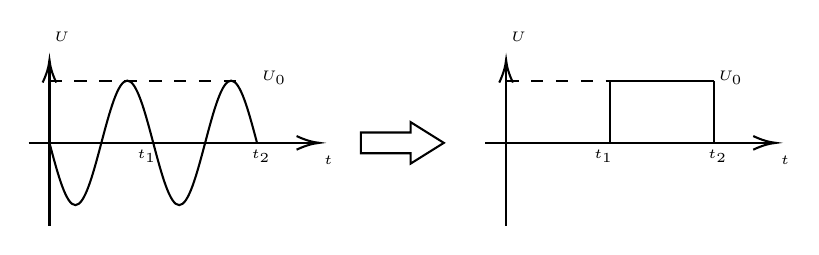
\begin{tikzpicture}[x=0.75pt,y=0.75pt,yscale=-1,xscale=1]
%uncomment if require: \path (0,300); %set diagram left start at 0, and has height of 300

%Shape: Wave [id:dp5957275904614414] 
\draw   (40,100) .. controls (44.08,115.37) and (47.98,130) .. (52.5,130) .. controls (57.02,130) and (60.92,115.37) .. (65,100) .. controls (69.08,84.63) and (72.98,70) .. (77.5,70) .. controls (82.02,70) and (85.92,84.63) .. (90,100) .. controls (94.08,115.37) and (97.98,130) .. (102.5,130) .. controls (107.02,130) and (110.92,115.37) .. (115,100) .. controls (119.08,84.63) and (122.98,70) .. (127.5,70) .. controls (132.02,70) and (135.92,84.63) .. (140,100) ;
%Straight Lines [id:da8807380521016539] 
\draw    (30,100) -- (168,100) ;
\draw [shift={(170,100)}, rotate = 180] [color={rgb, 255:red, 0; green, 0; blue, 0 }  ][line width=0.75]    (10.93,-3.29) .. controls (6.95,-1.4) and (3.31,-0.3) .. (0,0) .. controls (3.31,0.3) and (6.95,1.4) .. (10.93,3.29)   ;
%Straight Lines [id:da7234210438419781] 
\draw    (40,140) -- (40,62) ;
\draw [shift={(40,60)}, rotate = 90] [color={rgb, 255:red, 0; green, 0; blue, 0 }  ][line width=0.75]    (10.93,-3.29) .. controls (6.95,-1.4) and (3.31,-0.3) .. (0,0) .. controls (3.31,0.3) and (6.95,1.4) .. (10.93,3.29)   ;
%Straight Lines [id:da8881692477795176] 
\draw  [dash pattern={on 4.5pt off 4.5pt}]  (40,70) -- (130,70) ;
%Straight Lines [id:da7037740098329359] 
\draw    (250,100) -- (388,100) ;
\draw [shift={(390,100)}, rotate = 180] [color={rgb, 255:red, 0; green, 0; blue, 0 }  ][line width=0.75]    (10.93,-3.29) .. controls (6.95,-1.4) and (3.31,-0.3) .. (0,0) .. controls (3.31,0.3) and (6.95,1.4) .. (10.93,3.29)   ;
%Straight Lines [id:da24696901338014343] 
\draw    (260,140) -- (260,62) ;
\draw [shift={(260,60)}, rotate = 90] [color={rgb, 255:red, 0; green, 0; blue, 0 }  ][line width=0.75]    (10.93,-3.29) .. controls (6.95,-1.4) and (3.31,-0.3) .. (0,0) .. controls (3.31,0.3) and (6.95,1.4) .. (10.93,3.29)   ;
%Straight Lines [id:da028807109360900807] 
\draw  [dash pattern={on 4.5pt off 4.5pt}]  (260,70) -- (350,70) ;
%Right Arrow [id:dp35127513802390187] 
\draw   (190,95) -- (214,95) -- (214,90) -- (230,100) -- (214,110) -- (214,105) -- (190,105) -- cycle ;
%Straight Lines [id:da6668988615484821] 
\draw    (310,70) -- (310,100) ;
%Straight Lines [id:da5154013723623756] 
\draw    (360,70) -- (360,100) ;
%Straight Lines [id:da6769085058841795] 
\draw    (310,70) -- (360,70) ;

% Text Node
\draw (171,105) node [anchor=north west][inner sep=0.75pt]  [font=\tiny] [align=left] {$\displaystyle t$};
% Text Node
\draw (41,45) node [anchor=north west][inner sep=0.75pt]  [font=\tiny] [align=left] {$\displaystyle U$};
% Text Node
\draw (141,64) node [anchor=north west][inner sep=0.75pt]  [font=\tiny] [align=left] {$\displaystyle U_{0}$};
% Text Node
\draw (391,105) node [anchor=north west][inner sep=0.75pt]  [font=\tiny] [align=left] {$\displaystyle t$};
% Text Node
\draw (261,45) node [anchor=north west][inner sep=0.75pt]  [font=\tiny] [align=left] {$\displaystyle U$};
% Text Node
\draw (361,64) node [anchor=north west][inner sep=0.75pt]  [font=\tiny] [align=left] {$\displaystyle U_{0}$};
% Text Node
\draw (81,102) node [anchor=north west][inner sep=0.75pt]  [font=\tiny] [align=left] {$\displaystyle t_{1}$};
% Text Node
\draw (136,102) node [anchor=north west][inner sep=0.75pt]  [font=\tiny] [align=left] {$\displaystyle t_{2}$};
% Text Node
\draw (301,102) node [anchor=north west][inner sep=0.75pt]  [font=\tiny] [align=left] {$\displaystyle t_{1}$};
% Text Node
\draw (356,102) node [anchor=north west][inner sep=0.75pt]  [font=\tiny] [align=left] {$\displaystyle t_{2}$};


\end{tikzpicture}

\end{center}

运用以上方法,我们可以快速计算高中范围内所能见到的电压和电流的有效值,具体操作见下面例题。

\begin{ep}{自编题}{}
现有一交流电,其单个周期内波形如图所示,求该交流电有效值

\begin{center}
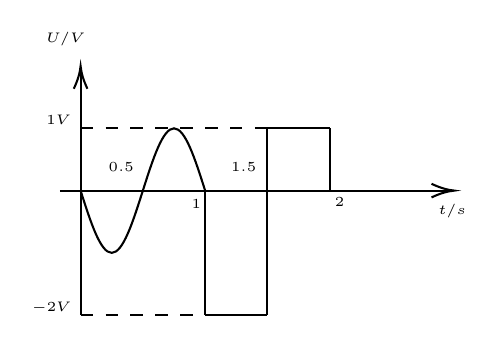
\begin{tikzpicture}[x=0.75pt,y=0.75pt,yscale=-1,xscale=1]
%uncomment if require: \path (0,300); %set diagram left start at 0, and has height of 300

%Shape: Wave [id:dp5957275904614414] 
\draw   (40,100) .. controls (44.89,115.37) and (49.57,130) .. (55,130) .. controls (60.43,130) and (65.11,115.37) .. (70,100) .. controls (74.89,84.63) and (79.57,70) .. (85,70) .. controls (90.43,70) and (95.11,84.63) .. (100,100) ;
%Straight Lines [id:da8807380521016539] 
\draw    (30,100) -- (167.3,100) -- (218,100) ;
\draw [shift={(220,100)}, rotate = 180] [color={rgb, 255:red, 0; green, 0; blue, 0 }  ][line width=0.75]    (10.93,-3.29) .. controls (6.95,-1.4) and (3.31,-0.3) .. (0,0) .. controls (3.31,0.3) and (6.95,1.4) .. (10.93,3.29)   ;
%Straight Lines [id:da7234210438419781] 
\draw    (40,160) -- (40,42) ;
\draw [shift={(40,40)}, rotate = 90] [color={rgb, 255:red, 0; green, 0; blue, 0 }  ][line width=0.75]    (10.93,-3.29) .. controls (6.95,-1.4) and (3.31,-0.3) .. (0,0) .. controls (3.31,0.3) and (6.95,1.4) .. (10.93,3.29)   ;
%Straight Lines [id:da8881692477795176] 
\draw  [dash pattern={on 4.5pt off 4.5pt}]  (40,70) -- (150,70) ;
%Straight Lines [id:da4109302093413363] 
\draw    (100,100) -- (100,160) ;
%Straight Lines [id:da7251683684825969] 
\draw    (100,160) -- (115.63,160) -- (130,160) ;
%Straight Lines [id:da6247280744273678] 
\draw  [dash pattern={on 4.5pt off 4.5pt}]  (40,160) -- (100,160) ;
%Straight Lines [id:da4811824903906994] 
\draw    (130,70) -- (130,160) ;
%Straight Lines [id:da07707215432170345] 
\draw    (130,70) -- (160,70) ;
%Straight Lines [id:da7362129417956969] 
\draw    (160,70) -- (160,100) ;

% Text Node
\draw (211,105) node [anchor=north west][inner sep=0.75pt]  [font=\tiny] [align=left] {$\displaystyle t/s$};
% Text Node
\draw (22,22) node [anchor=north west][inner sep=0.75pt]  [font=\tiny] [align=left] {$\displaystyle U/V$};
% Text Node
\draw (22,62) node [anchor=north west][inner sep=0.75pt]  [font=\tiny] [align=left] {$\displaystyle 1V$};
% Text Node
\draw (92,103) node [anchor=north west][inner sep=0.75pt]  [font=\tiny] [align=left] {$\displaystyle 1$};
% Text Node
\draw (161,102) node [anchor=north west][inner sep=0.75pt]  [font=\tiny] [align=left] {$\displaystyle 2$};
% Text Node
\draw (15,152) node [anchor=north west][inner sep=0.75pt]  [font=\tiny] [align=left] {$\displaystyle -2V$};
% Text Node
\draw (111,85) node [anchor=north west][inner sep=0.75pt]  [font=\tiny] [align=left] {$\displaystyle 1.5$};
% Text Node
\draw (52,85) node [anchor=north west][inner sep=0.75pt]  [font=\tiny] [align=left] {$\displaystyle 0.5$};


\end{tikzpicture}

\end{center}

首先,我们先把正弦波等效为方波,根据前文\theoref{zxbdxfb},有

\begin{center}
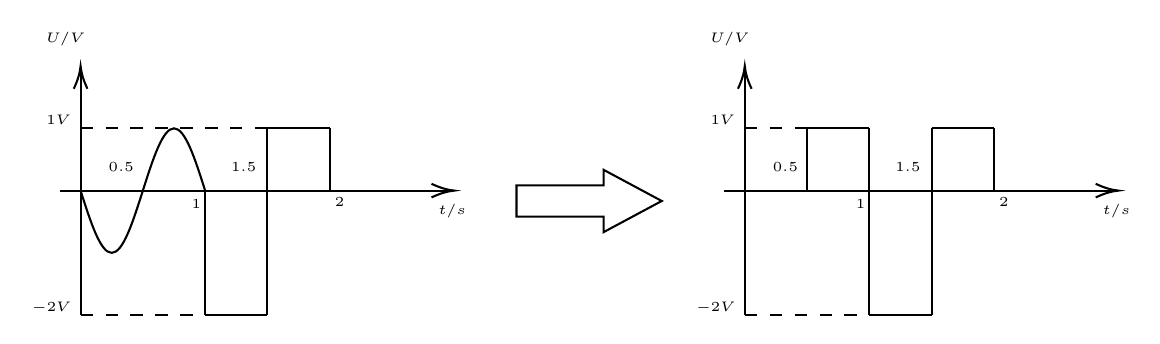
\begin{tikzpicture}[x=0.75pt,y=0.75pt,yscale=-1,xscale=1]
%uncomment if require: \path (0,300); %set diagram left start at 0, and has height of 300

%Shape: Wave [id:dp5957275904614414] 
\draw   (40,100) .. controls (44.89,115.37) and (49.57,130) .. (55,130) .. controls (60.43,130) and (65.11,115.37) .. (70,100) .. controls (74.89,84.63) and (79.57,70) .. (85,70) .. controls (90.43,70) and (95.11,84.63) .. (100,100) ;
%Straight Lines [id:da8807380521016539] 
\draw    (30,100) -- (167.3,100) -- (218,100) ;
\draw [shift={(220,100)}, rotate = 180] [color={rgb, 255:red, 0; green, 0; blue, 0 }  ][line width=0.75]    (10.93,-3.29) .. controls (6.95,-1.4) and (3.31,-0.3) .. (0,0) .. controls (3.31,0.3) and (6.95,1.4) .. (10.93,3.29)   ;
%Straight Lines [id:da7234210438419781] 
\draw    (40,160) -- (40,42) ;
\draw [shift={(40,40)}, rotate = 90] [color={rgb, 255:red, 0; green, 0; blue, 0 }  ][line width=0.75]    (10.93,-3.29) .. controls (6.95,-1.4) and (3.31,-0.3) .. (0,0) .. controls (3.31,0.3) and (6.95,1.4) .. (10.93,3.29)   ;
%Straight Lines [id:da8881692477795176] 
\draw  [dash pattern={on 4.5pt off 4.5pt}]  (40,70) -- (150,70) ;
%Straight Lines [id:da4109302093413363] 
\draw    (100,100) -- (100,160) ;
%Straight Lines [id:da7251683684825969] 
\draw    (100,160) -- (115.63,160) -- (130,160) ;
%Straight Lines [id:da6247280744273678] 
\draw  [dash pattern={on 4.5pt off 4.5pt}]  (40,160) -- (100,160) ;
%Straight Lines [id:da4811824903906994] 
\draw    (130,70) -- (130,160) ;
%Straight Lines [id:da07707215432170345] 
\draw    (130,70) -- (160,70) ;
%Straight Lines [id:da7362129417956969] 
\draw    (160,70) -- (160,100) ;
%Right Arrow [id:dp2964750951442603] 
\draw   (250,97.5) -- (292,97.5) -- (292,90) -- (320,105) -- (292,120) -- (292,112.5) -- (250,112.5) -- cycle ;
%Straight Lines [id:da09767427738803702] 
\draw    (350,100) -- (487.3,100) -- (538,100) ;
\draw [shift={(540,100)}, rotate = 180] [color={rgb, 255:red, 0; green, 0; blue, 0 }  ][line width=0.75]    (10.93,-3.29) .. controls (6.95,-1.4) and (3.31,-0.3) .. (0,0) .. controls (3.31,0.3) and (6.95,1.4) .. (10.93,3.29)   ;
%Straight Lines [id:da14812927937967957] 
\draw    (360,160) -- (360,42) ;
\draw [shift={(360,40)}, rotate = 90] [color={rgb, 255:red, 0; green, 0; blue, 0 }  ][line width=0.75]    (10.93,-3.29) .. controls (6.95,-1.4) and (3.31,-0.3) .. (0,0) .. controls (3.31,0.3) and (6.95,1.4) .. (10.93,3.29)   ;
%Straight Lines [id:da18788096109920538] 
\draw    (420,70) -- (420,160) ;
%Straight Lines [id:da8582172719266195] 
\draw    (420,160) -- (435.63,160) -- (450,160) ;
%Straight Lines [id:da198364716671944] 
\draw  [dash pattern={on 4.5pt off 4.5pt}]  (360,160) -- (420,160) ;
%Straight Lines [id:da052239762684211044] 
\draw    (450,70) -- (450,160) ;
%Straight Lines [id:da06018736260010238] 
\draw    (450,70) -- (480,70) ;
%Straight Lines [id:da6522253327127172] 
\draw    (480,70) -- (480,100) ;
%Straight Lines [id:da41909877434480447] 
\draw    (390,70) -- (390,100) ;
%Straight Lines [id:da42513251191113355] 
\draw    (390,70) -- (420,70) ;
%Straight Lines [id:da6695934984306693] 
\draw  [dash pattern={on 4.5pt off 4.5pt}]  (360,70) -- (390,70) ;

% Text Node
\draw (211,105) node [anchor=north west][inner sep=0.75pt]  [font=\tiny] [align=left] {$\displaystyle t/s$};
% Text Node
\draw (22,22) node [anchor=north west][inner sep=0.75pt]  [font=\tiny] [align=left] {$\displaystyle U/V$};
% Text Node
\draw (22,62) node [anchor=north west][inner sep=0.75pt]  [font=\tiny] [align=left] {$\displaystyle 1V$};
% Text Node
\draw (92,103) node [anchor=north west][inner sep=0.75pt]  [font=\tiny] [align=left] {$\displaystyle 1$};
% Text Node
\draw (161,102) node [anchor=north west][inner sep=0.75pt]  [font=\tiny] [align=left] {$\displaystyle 2$};
% Text Node
\draw (15,152) node [anchor=north west][inner sep=0.75pt]  [font=\tiny] [align=left] {$\displaystyle -2V$};
% Text Node
\draw (111,85) node [anchor=north west][inner sep=0.75pt]  [font=\tiny] [align=left] {$\displaystyle 1.5$};
% Text Node
\draw (52,85) node [anchor=north west][inner sep=0.75pt]  [font=\tiny] [align=left] {$\displaystyle 0.5$};
% Text Node
\draw (531,105) node [anchor=north west][inner sep=0.75pt]  [font=\tiny] [align=left] {$\displaystyle t/s$};
% Text Node
\draw (342,22) node [anchor=north west][inner sep=0.75pt]  [font=\tiny] [align=left] {$\displaystyle U/V$};
% Text Node
\draw (342,62) node [anchor=north west][inner sep=0.75pt]  [font=\tiny] [align=left] {$\displaystyle 1V$};
% Text Node
\draw (412,103) node [anchor=north west][inner sep=0.75pt]  [font=\tiny] [align=left] {$\displaystyle 1$};
% Text Node
\draw (481,102) node [anchor=north west][inner sep=0.75pt]  [font=\tiny] [align=left] {$\displaystyle 2$};
% Text Node
\draw (335,152) node [anchor=north west][inner sep=0.75pt]  [font=\tiny] [align=left] {$\displaystyle -2V$};
% Text Node
\draw (431,85) node [anchor=north west][inner sep=0.75pt]  [font=\tiny] [align=left] {$\displaystyle 1.5$};
% Text Node
\draw (372,85) node [anchor=north west][inner sep=0.75pt]  [font=\tiny] [align=left] {$\displaystyle 0.5$};
\end{tikzpicture}
\end{center}

因此,我们可以看到,等效后整个波形由两个电压组成,$1V$电压持续了$1s$,占了整个波形的$\frac{1}{2}$。而$2V$电压(\textbf{计算有效值时我们不考虑正负})持续了$0.5s$,占了整个波形的$\frac{1}{4}$。因此,由均方根值计算公式,有

$$U_{eq} = \sqrt{\frac{1}{2} \times 1^2 + \frac{1}{4} \times 2^2} = \frac{\sqrt{6}}{2}$$

此方法熟练后,如果题目数据设置比较易算,我们可以直接口算出有效值。

\end{ep}

\section{正则动量}

\begin{center}

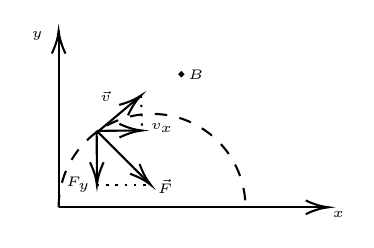
\begin{tikzpicture}[x=0.75pt,y=0.75pt,yscale=-1,xscale=1]
%uncomment if require: \path (0,300); %set diagram left start at 0, and has height of 300

%Shape: Arc [id:dp14057216895852598] 
\draw  [draw opacity=0][dash pattern={on 4.5pt off 4.5pt}] (100,175) .. controls (100,175) and (100,175) .. (100,175) .. controls (100,150.15) and (120.15,130) .. (145,130) .. controls (169.85,130) and (190,150.15) .. (190,175) -- (145,175) -- cycle ; \draw  [dash pattern={on 4.5pt off 4.5pt}] (100,175) .. controls (100,175) and (100,175) .. (100,175) .. controls (100,150.15) and (120.15,130) .. (145,130) .. controls (169.85,130) and (190,150.15) .. (190,175) ;  
%Straight Lines [id:da08657086057780239] 
\draw    (100,175) -- (228,175) ;
\draw [shift={(230,175)}, rotate = 180] [color={rgb, 255:red, 0; green, 0; blue, 0 }  ][line width=0.75]    (10.93,-3.29) .. controls (6.95,-1.4) and (3.31,-0.3) .. (0,0) .. controls (3.31,0.3) and (6.95,1.4) .. (10.93,3.29)   ;
%Straight Lines [id:da6524966000913504] 
\draw    (100,175) -- (100,92) ;
\draw [shift={(100,90)}, rotate = 90] [color={rgb, 255:red, 0; green, 0; blue, 0 }  ][line width=0.75]    (10.93,-3.29) .. controls (6.95,-1.4) and (3.31,-0.3) .. (0,0) .. controls (3.31,0.3) and (6.95,1.4) .. (10.93,3.29)   ;
%Straight Lines [id:da7289215350120348] 
\draw    (118,139.33) -- (138.14,122.43) ;
\draw [shift={(139.67,121.15)}, rotate = 140] [color={rgb, 255:red, 0; green, 0; blue, 0 }  ][line width=0.75]    (10.93,-3.29) .. controls (6.95,-1.4) and (3.31,-0.3) .. (0,0) .. controls (3.31,0.3) and (6.95,1.4) .. (10.93,3.29)   ;
%Shape: Circle [id:dp25826008472643713] 
\draw  [fill={rgb, 255:red, 0; green, 0; blue, 0 }  ,fill opacity=1 ] (158.25,110.88) .. controls (158.25,110.39) and (158.64,110) .. (159.12,110) .. controls (159.61,110) and (160,110.39) .. (160,110.88) .. controls (160,111.36) and (159.61,111.75) .. (159.12,111.75) .. controls (158.64,111.75) and (158.25,111.36) .. (158.25,110.88) -- cycle ;
%Straight Lines [id:da4913512294964639] 
\draw    (118.33,138.18) -- (138.19,138.04) ;
\draw [shift={(140.19,138.02)}, rotate = 179.58] [color={rgb, 255:red, 0; green, 0; blue, 0 }  ][line width=0.75]    (10.93,-3.29) .. controls (6.95,-1.4) and (3.31,-0.3) .. (0,0) .. controls (3.31,0.3) and (6.95,1.4) .. (10.93,3.29)   ;
%Straight Lines [id:da1860456917216915] 
\draw  [dash pattern={on 0.84pt off 2.51pt}]  (139.67,121.15) -- (140.19,138.02) ;
%Straight Lines [id:da8050183117692913] 
\draw    (118.33,138.18) -- (118.43,162.27) ;
\draw [shift={(118.44,164.27)}, rotate = 269.76] [color={rgb, 255:red, 0; green, 0; blue, 0 }  ][line width=0.75]    (10.93,-3.29) .. controls (6.95,-1.4) and (3.31,-0.3) .. (0,0) .. controls (3.31,0.3) and (6.95,1.4) .. (10.93,3.29)   ;
%Straight Lines [id:da977236805798956] 
\draw    (118.33,138.18) -- (143.02,162.86) ;
\draw [shift={(144.44,164.27)}, rotate = 224.98] [color={rgb, 255:red, 0; green, 0; blue, 0 }  ][line width=0.75]    (10.93,-3.29) .. controls (6.95,-1.4) and (3.31,-0.3) .. (0,0) .. controls (3.31,0.3) and (6.95,1.4) .. (10.93,3.29)   ;
%Straight Lines [id:da3726775979597923] 
\draw  [dash pattern={on 0.84pt off 2.51pt}]  (118.44,164.27) -- (144.44,164.27) ;

% Text Node
\draw (230.58,175.63) node [anchor=north west][inner sep=0.75pt]  [font=\tiny]  {$x$};
% Text Node
\draw (85.58,88.97) node [anchor=north west][inner sep=0.75pt]  [font=\tiny]  {$y$};
% Text Node
\draw (118.66,117.88) node [anchor=north west][inner sep=0.75pt]  [font=\tiny]  {$\vec{v}$};
% Text Node
\draw (161,107.4) node [anchor=north west][inner sep=0.75pt]  [font=\tiny]  {$B$};
% Text Node
\draw (143,133.15) node [anchor=north west][inner sep=0.75pt]  [font=\tiny]  {$v_{x}$};
% Text Node
\draw (102.25,158.9) node [anchor=north west][inner sep=0.75pt]  [font=\tiny]  {$F_{y}$};
% Text Node
\draw (146.25,160.15) node [anchor=north west][inner sep=0.75pt]  [font=\tiny]  {$\vec{F}$};


\end{tikzpicture}

\end{center}
如图所示,在垂直纸面向外的磁场$B$中有一个质量为$m$,电荷为$q$的带正电荷粒子初始时以速度$v$沿着$y$轴运动。由洛伦兹力得

$$F_y = B q v_x$$

上式中$F_y$方向为沿着$y$轴负方向(略去了仅代表方向的负号,只考虑大小),上式两端乘$\Delta t$,得

$$\Delta P_y = F_y \Delta t = B q v_x \Delta t = B q \Delta x$$

\begin{theo}{正则动量}{}
粒子在$x$方向上的位移$\Delta x$与在$y$方向上的动量改变量$\Delta P_y$满足

$$\Delta P_y = B q \Delta x$$

其中$\Delta P_y$的方向遵循左手定则\footnote{这里是化简的写法,在大学物理中,电磁场中正则动量为$\hat{P} = m \vec{v} + q \vec{A}$,其中$\vec{A}$为磁矢势。正则动量在磁场中守恒。对于前文所提匀强磁场,$\hat{P_y} = m v_y + B q x$,初末态$\hat{P}$相等,化简得出上式。也因此此方法其实就是正则动量守恒}。

\end{theo}

这里我们可以举一个我们再熟悉不过的例子验证此式子的正确。我们知道,带电粒子只受磁场力且在垂直磁场平面运动时为圆周运动,满足

$$B q v = m \frac{v^2}{R}$$

当粒子运动了$\frac{1}{4}$圆周时,其$y$方向动量改变$\Delta P_y$,因此由正则动量守恒,有

$$\Delta x = \frac{\Delta P_y}{B q} = \frac{m v}{B q}$$

可以看到就是我们所熟悉的粒子运动半径$R$,由图示可知$\Delta x$确实等于$R$。

\section{“同吸反斥”}

\begin{center}

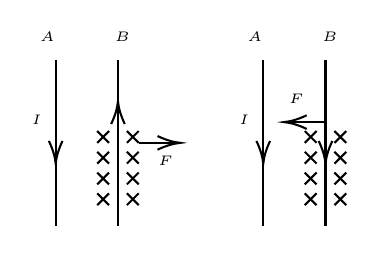
\begin{tikzpicture}[x=0.75pt,y=0.75pt,yscale=-1,xscale=1]
%uncomment if require: \path (0,300); %set diagram left start at 0, and has height of 300

%Straight Lines [id:da9726211238858622] 
\draw    (140,70) -- (140,150) ;
%Straight Lines [id:da7695426039962214] 
\draw    (170,70) -- (170,150) ;
%Straight Lines [id:da8260247386172599] 
\draw    (140,90) -- (140,118) ;
\draw [shift={(140,120)}, rotate = 270] [color={rgb, 255:red, 0; green, 0; blue, 0 }  ][line width=0.75]    (10.93,-3.29) .. controls (6.95,-1.4) and (3.31,-0.3) .. (0,0) .. controls (3.31,0.3) and (6.95,1.4) .. (10.93,3.29)   ;
%Straight Lines [id:da7709293981109604] 
\draw    (170,120) -- (170,92) ;
\draw [shift={(170,90)}, rotate = 90] [color={rgb, 255:red, 0; green, 0; blue, 0 }  ][line width=0.75]    (10.93,-3.29) .. controls (6.95,-1.4) and (3.31,-0.3) .. (0,0) .. controls (3.31,0.3) and (6.95,1.4) .. (10.93,3.29)   ;
%Straight Lines [id:da4626627845879374] 
\draw    (180,110) -- (198,110) ;
\draw [shift={(200,110)}, rotate = 180] [color={rgb, 255:red, 0; green, 0; blue, 0 }  ][line width=0.75]    (10.93,-3.29) .. controls (6.95,-1.4) and (3.31,-0.3) .. (0,0) .. controls (3.31,0.3) and (6.95,1.4) .. (10.93,3.29)   ;
%Straight Lines [id:da7556852046106817] 
\draw    (174.3,104.3) -- (180,110) ;
%Straight Lines [id:da3056633172798764] 
\draw    (180,104.3) -- (174.3,110) ;

%Straight Lines [id:da869864321489574] 
\draw    (160,104.3) -- (165.7,110) ;
%Straight Lines [id:da7393063880787207] 
\draw    (165.7,104.3) -- (160,110) ;

%Straight Lines [id:da8750050188826155] 
\draw    (174.3,114.3) -- (180,120) ;
%Straight Lines [id:da11301530874135057] 
\draw    (180,114.3) -- (174.3,120) ;

%Straight Lines [id:da49493004908563787] 
\draw    (160,114.3) -- (165.7,120) ;
%Straight Lines [id:da30954199680164174] 
\draw    (165.7,114.3) -- (160,120) ;

%Straight Lines [id:da8531640047364577] 
\draw    (174.3,124.3) -- (180,130) ;
%Straight Lines [id:da44587483395009175] 
\draw    (180,124.3) -- (174.3,130) ;

%Straight Lines [id:da42443043610212694] 
\draw    (160,124.3) -- (165.7,130) ;
%Straight Lines [id:da9188692663482869] 
\draw    (165.7,124.3) -- (160,130) ;

%Straight Lines [id:da41788523071131123] 
\draw    (174.3,134.3) -- (180,140) ;
%Straight Lines [id:da9544792756550795] 
\draw    (180,134.3) -- (174.3,140) ;

%Straight Lines [id:da4433110870124555] 
\draw    (160,134.3) -- (165.7,140) ;
%Straight Lines [id:da6800629739118609] 
\draw    (165.7,134.3) -- (160,140) ;

%Straight Lines [id:da8440880013672787] 
\draw    (240,70) -- (240,150) ;
%Straight Lines [id:da057150037628339145] 
\draw    (270,70) -- (270,150) ;
%Straight Lines [id:da2742462831123351] 
\draw    (240,90) -- (240,118) ;
\draw [shift={(240,120)}, rotate = 270] [color={rgb, 255:red, 0; green, 0; blue, 0 }  ][line width=0.75]    (10.93,-3.29) .. controls (6.95,-1.4) and (3.31,-0.3) .. (0,0) .. controls (3.31,0.3) and (6.95,1.4) .. (10.93,3.29)   ;
%Straight Lines [id:da4841221810696197] 
\draw    (270,90) -- (270,118) ;
\draw [shift={(270,120)}, rotate = 270] [color={rgb, 255:red, 0; green, 0; blue, 0 }  ][line width=0.75]    (10.93,-3.29) .. controls (6.95,-1.4) and (3.31,-0.3) .. (0,0) .. controls (3.31,0.3) and (6.95,1.4) .. (10.93,3.29)   ;
%Straight Lines [id:da41148702267178616] 
\draw    (270,100) -- (252,100) ;
\draw [shift={(250,100)}, rotate = 360] [color={rgb, 255:red, 0; green, 0; blue, 0 }  ][line width=0.75]    (10.93,-3.29) .. controls (6.95,-1.4) and (3.31,-0.3) .. (0,0) .. controls (3.31,0.3) and (6.95,1.4) .. (10.93,3.29)   ;
%Straight Lines [id:da4874107654826265] 
\draw    (274.3,104.3) -- (280,110) ;
%Straight Lines [id:da3209563362299912] 
\draw    (280,104.3) -- (274.3,110) ;

%Straight Lines [id:da5685878086287939] 
\draw    (260,104.3) -- (265.7,110) ;
%Straight Lines [id:da4644596696434773] 
\draw    (265.7,104.3) -- (260,110) ;

%Straight Lines [id:da3255281963831984] 
\draw    (274.3,114.3) -- (280,120) ;
%Straight Lines [id:da3659699288633731] 
\draw    (280,114.3) -- (274.3,120) ;

%Straight Lines [id:da9401441995552069] 
\draw    (260,114.3) -- (265.7,120) ;
%Straight Lines [id:da35693277494486786] 
\draw    (265.7,114.3) -- (260,120) ;

%Straight Lines [id:da5739270247855444] 
\draw    (274.3,124.3) -- (280,130) ;
%Straight Lines [id:da519349341958852] 
\draw    (280,124.3) -- (274.3,130) ;

%Straight Lines [id:da32740686649303874] 
\draw    (260,124.3) -- (265.7,130) ;
%Straight Lines [id:da24227504756826423] 
\draw    (265.7,124.3) -- (260,130) ;

%Straight Lines [id:da4688572412478589] 
\draw    (274.3,134.3) -- (280,140) ;
%Straight Lines [id:da031095938355117703] 
\draw    (280,134.3) -- (274.3,140) ;

%Straight Lines [id:da6487424748031143] 
\draw    (260,134.3) -- (265.7,140) ;
%Straight Lines [id:da5986743936375074] 
\draw    (265.7,134.3) -- (260,140) ;


% Text Node
\draw (131,55) node [anchor=north west][inner sep=0.75pt]  [font=\tiny] [align=left] {$\displaystyle A$};
% Text Node
\draw (167,55) node [anchor=north west][inner sep=0.75pt]  [font=\tiny] [align=left] {$\displaystyle B$};
% Text Node
\draw (188,115) node [anchor=north west][inner sep=0.75pt]  [font=\tiny] [align=left] {$\displaystyle F$};
% Text Node
\draw (127,95) node [anchor=north west][inner sep=0.75pt]  [font=\tiny] [align=left] {$\displaystyle I$};
% Text Node
\draw (231,55) node [anchor=north west][inner sep=0.75pt]  [font=\tiny] [align=left] {$\displaystyle A$};
% Text Node
\draw (267,55) node [anchor=north west][inner sep=0.75pt]  [font=\tiny] [align=left] {$\displaystyle B$};
% Text Node
\draw (251,85) node [anchor=north west][inner sep=0.75pt]  [font=\tiny] [align=left] {$\displaystyle F$};
% Text Node
\draw (227,95) node [anchor=north west][inner sep=0.75pt]  [font=\tiny] [align=left] {$\displaystyle I$};


\end{tikzpicture}

\end{center}

对于两根通电导线,若两根导线电流方向相反,如左图所示,根据安培定则以及右手螺旋定则,则两根导线相互排斥;同理,若两根导线电流方向相同,则两根导线相互吸引。

\begin{theo}{“同吸反斥”}{}
\textbf{电流总有趋向于同向的趋势,同向电流相互吸引,反向电流相互排斥},即“同吸反斥”。
\end{theo}

此定理可以和楞次定律的“增反减同”、“来拒去留”、“增缩减扩”一同记忆,在解决电磁感应下导线受力问题时常常能极大简化分析,具体操作见如下例题。

\section{电磁场换系}
\label{s_dcchx}

\begin{center}

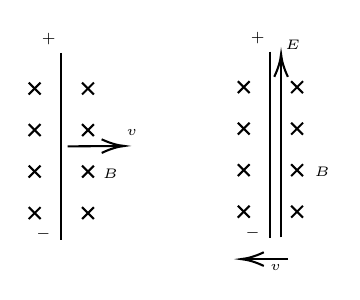
\begin{tikzpicture}[x=0.75pt,y=0.75pt,yscale=-1,xscale=1]
%uncomment if require: \path (0,300); %set diagram left start at 0, and has height of 300

%Straight Lines [id:da7695426039962214] 
\draw    (170,60) -- (170,150) ;
%Straight Lines [id:da7556852046106817] 
\draw    (180,74.3) -- (185.7,80) ;
%Straight Lines [id:da3056633172798764] 
\draw    (185.7,74.3) -- (180,80) ;

%Straight Lines [id:da869864321489574] 
\draw    (154.3,74.3) -- (160,80) ;
%Straight Lines [id:da7393063880787207] 
\draw    (160,74.3) -- (154.3,80) ;

%Straight Lines [id:da8750050188826155] 
\draw    (180,94.3) -- (185.7,100) ;
%Straight Lines [id:da11301530874135057] 
\draw    (185.7,94.3) -- (180,100) ;

%Straight Lines [id:da49493004908563787] 
\draw    (154.3,94.3) -- (160,100) ;
%Straight Lines [id:da30954199680164174] 
\draw    (160,94.3) -- (154.3,100) ;

%Straight Lines [id:da8531640047364577] 
\draw    (180,114.3) -- (185.7,120) ;
%Straight Lines [id:da44587483395009175] 
\draw    (185.7,114.3) -- (180,120) ;

%Straight Lines [id:da42443043610212694] 
\draw    (154.3,114.3) -- (160,120) ;
%Straight Lines [id:da9188692663482869] 
\draw    (160,114.3) -- (154.3,120) ;

%Straight Lines [id:da41788523071131123] 
\draw    (180,134.3) -- (185.7,140) ;
%Straight Lines [id:da9544792756550795] 
\draw    (185.7,134.3) -- (180,140) ;

%Straight Lines [id:da4433110870124555] 
\draw    (154.3,134.3) -- (160,140) ;
%Straight Lines [id:da6800629739118609] 
\draw    (160,134.3) -- (154.3,140) ;

%Straight Lines [id:da43990185383735314] 
\draw    (173,105) -- (198.38,104.84) ;
\draw [shift={(200.38,104.82)}, rotate = 179.63] [color={rgb, 255:red, 0; green, 0; blue, 0 }  ][line width=0.75]    (10.93,-3.29) .. controls (6.95,-1.4) and (3.31,-0.3) .. (0,0) .. controls (3.31,0.3) and (6.95,1.4) .. (10.93,3.29)   ;
%Straight Lines [id:da447256886640123] 
\draw    (270.75,59.32) -- (270.75,149.32) ;
%Straight Lines [id:da8108904848429168] 
\draw    (280.75,73.62) -- (286.45,79.32) ;
%Straight Lines [id:da22647656640350244] 
\draw    (286.45,73.62) -- (280.75,79.32) ;

%Straight Lines [id:da04493093294125461] 
\draw    (255.05,73.62) -- (260.75,79.32) ;
%Straight Lines [id:da44087585195785506] 
\draw    (260.75,73.62) -- (255.05,79.32) ;

%Straight Lines [id:da14075284118411946] 
\draw    (280.75,93.62) -- (286.45,99.32) ;
%Straight Lines [id:da9617822087320003] 
\draw    (286.45,93.62) -- (280.75,99.32) ;

%Straight Lines [id:da2241357731693263] 
\draw    (255.05,93.62) -- (260.75,99.32) ;
%Straight Lines [id:da3543204736554191] 
\draw    (260.75,93.62) -- (255.05,99.32) ;

%Straight Lines [id:da6424389047712769] 
\draw    (280.75,113.62) -- (286.45,119.32) ;
%Straight Lines [id:da8372903681478225] 
\draw    (286.45,113.62) -- (280.75,119.32) ;

%Straight Lines [id:da22862218634462628] 
\draw    (255.05,113.62) -- (260.75,119.32) ;
%Straight Lines [id:da4701024632645656] 
\draw    (260.75,113.62) -- (255.05,119.32) ;

%Straight Lines [id:da48139298541867737] 
\draw    (280.75,133.62) -- (286.45,139.32) ;
%Straight Lines [id:da506331558201988] 
\draw    (286.45,133.62) -- (280.75,139.32) ;

%Straight Lines [id:da0678654926298945] 
\draw    (255.05,133.62) -- (260.75,139.32) ;
%Straight Lines [id:da36131022791916534] 
\draw    (260.75,133.62) -- (255.05,139.32) ;

%Straight Lines [id:da4285683783673411] 
\draw    (279.25,159.32) -- (258.63,159.32) ;
\draw [shift={(256.63,159.32)}, rotate = 359.99] [color={rgb, 255:red, 0; green, 0; blue, 0 }  ][line width=0.75]    (10.93,-3.29) .. controls (6.95,-1.4) and (3.31,-0.3) .. (0,0) .. controls (3.31,0.3) and (6.95,1.4) .. (10.93,3.29)   ;
%Straight Lines [id:da7794422427057781] 
\draw    (275.88,148.82) -- (275.88,62.57) ;
\draw [shift={(275.88,60.57)}, rotate = 90] [color={rgb, 255:red, 0; green, 0; blue, 0 }  ][line width=0.75]    (10.93,-3.29) .. controls (6.95,-1.4) and (3.31,-0.3) .. (0,0) .. controls (3.31,0.3) and (6.95,1.4) .. (10.93,3.29)   ;

% Text Node
\draw (188.5,114.5) node [anchor=north west][inner sep=0.75pt]  [font=\tiny] [align=left] {$\displaystyle B$};
% Text Node
\draw (200,95.5) node [anchor=north west][inner sep=0.75pt]  [font=\tiny] [align=left] {$\displaystyle v$};
% Text Node
\draw (159,49) node [anchor=north west][inner sep=0.75pt]  [font=\tiny] [align=left] {$\displaystyle +$};
% Text Node
\draw (156.3,143) node [anchor=north west][inner sep=0.75pt]  [font=\tiny] [align=left] {$\displaystyle -$};
% Text Node
\draw (290.5,113.57) node [anchor=north west][inner sep=0.75pt]  [font=\tiny] [align=left] {$\displaystyle B$};
% Text Node
\draw (269.25,160.32) node [anchor=north west][inner sep=0.75pt]  [font=\tiny] [align=left] {$\displaystyle v$};
% Text Node
\draw (259.75,48.32) node [anchor=north west][inner sep=0.75pt]  [font=\tiny] [align=left] {$\displaystyle +$};
% Text Node
\draw (257.05,142.32) node [anchor=north west][inner sep=0.75pt]  [font=\tiny] [align=left] {$\displaystyle -$};
% Text Node
\draw (276.5,52.32) node [anchor=north west][inner sep=0.75pt]  [font=\tiny] [align=left] {$\displaystyle E$};


\end{tikzpicture}

\end{center}

如图左图所示,若在一个大小为$B$的匀强磁场中存在一根长为$L$的金属杆以速度$v$切割磁感线,那么金属杆两端的电动势为$\ms E = B L v$;但我们还可以在另一个参考系考虑这个问题。如右图所示,\textbf{我们以金属杆为参照选取参考系},那么在新参考系中,金属杆速度为$0$,而磁场以速度$v$向左运动。\textbf{由于改变参考系不应改变杆两端的电势差,故我们可以认为在新参考系中存在一个方向向上的电场$E$},其电场大小满足$E L = B L v$,即$E = B v$,方向可用左图由右手定则判断(跟判断动生电动势相同,但将电流当成电场,电流方向即电场方向。当然也可以用后面的\secref{s_tyzsdz}或者下文的叉乘式(式\eqref{e_dcchx_cc})判断方向)。

故我们可以得到电磁场换系的变换关系

\begin{theo}[label=d_dcchx]{电磁场换系}{}
若在参考系$S$中存在匀强磁场$B$(为讨论方便,取原电场为0),现有新参考系$S^{\prime}$相对旧参考系$S$以速度$v$运动,在新参考系$S^{\prime}$中,其等效的磁场$B^{\prime}$,电场$E^{\prime}$满足

$$B^{\prime} = B, \quad E^{\prime} = B v$$

其中$E^{\prime}$方向可在$S$系中由右手定则确定。

\end{theo}

\begin{mk}{更严谨的推导(超纲)}{}
对于上文电磁场换系,其本质上是电磁场的相对论变换,其需要竞赛的一些知识,在此不做介绍,感兴趣的同学可自行搜索有关内容。以下给出其简略推导过程
~\\

电磁场满足洛伦兹变换,从$S$系变换到$S^{\prime}$系满足

$$\vec{E^{\prime}} = \gamma (\vec{E} - \vec{v} \times \vec{B}), \quad \vec{B^{\prime}} = \gamma (\vec{B} +\frac{\vec{v} \times \vec{E}}{c^2}), \quad \gamma = \frac{1}{\sqrt{1-(\frac{v}{c})^2}}$$

其中$\gamma$为洛伦兹因子,“$\times$”为叉乘(见\defiref{d_cc})。在低速中($v \ll c$),$\gamma = 1$,$(\vec{v} \times \vec{E})/c^2 = 0$,故上式化简为
$$\vec{E^{\prime}} = \vec{E} - \vec{v} \times \vec{B}, \quad \vec{B^{\prime}} = \vec{B}$$

取原电场场强为$\vec{0}$,由叉乘的反交换律\eqref{d_cc},得

\begin{equation}
\label{e_dcchx_cc}
\boxed{\vec{E^{\prime}} = \vec{B} \times \vec{v}, \quad \vec{B^{\prime}} = \vec{B}}
\end{equation}

即前文公式的矢量式。
\end{mk}

\section{配速法}

\iffalse
\subsection{运动独立性原则}

在介绍配速法前,先介绍一下配速法的一个重要的理论基础

\begin{theo}[label=d_yddlx]{运动独立性原则}{}
运动独立性原则,是指一个物体同时参与几种运动,各分运动都可看成独立进行的,互不影响,\textbf{物体的合运动则视为几个相互独立分运动叠加的结果}。
\end{theo}

在高中阶段,上面的定理经常被用于处理平抛运动,$x$方向上的匀速运动和$y$方向上的自由落体,互不影响。而物体的合运动则为$x$方向上运动和$y$方向上运动的叠加。

我们可以将上面的定律进行推广,我们在进行速度的分解时并不一定要进行正交分解\footnote{“正交”指分解的两个矢量相互垂直},\textbf{我们可以通过平行四边形法则任意分解,其合运动仍旧为几个相互独立分运动叠加的结果}。而一般我们进行正交分解只是因为其便于讨论。

\subsection{配速法}
\fi

\subsection{分解速度角度介绍“配速法”}

何为“配速法”?配速法其实就是将原来速度分解,给物体配一个速度$\vec{v}$,使得这个速度所产生的洛伦兹力与题中的重力或者电场力(视情况而定)抵消,对应的,这时还会剩下一个速度$\vec{v^{\prime}}$,这时等效于只受到一个洛伦兹力,而不再是重力或者电场力加上洛伦兹力,从而降低分析难度。

\begin{center}
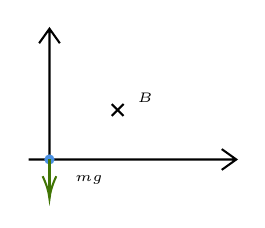
\begin{tikzpicture}[x=0.75pt,y=0.75pt,yscale=-1,xscale=1]
%uncomment if require: \path (0,300); %set diagram left start at 0, and has height of 300

%Straight Lines [id:da869864321489574] 
\draw    (210,94.3) -- (215.7,100) ;
%Straight Lines [id:da7393063880787207] 
\draw    (215.7,94.3) -- (210,100) ;

%Shape: Axis 2D [id:dp2610193597490549] 
\draw  (170,121) -- (270,121)(180,58) -- (180,128) (263,116) -- (270,121) -- (263,126) (175,65) -- (180,58) -- (185,65)  ;
%Shape: Circle [id:dp711598281784179] 
\draw  [color={rgb, 255:red, 74; green, 144; blue, 226 }  ,draw opacity=1 ][fill={rgb, 255:red, 74; green, 144; blue, 226 }  ,fill opacity=1 ] (178.09,121) .. controls (178.09,119.94) and (178.94,119.09) .. (180,119.09) .. controls (181.06,119.09) and (181.91,119.94) .. (181.91,121) .. controls (181.91,122.06) and (181.06,122.91) .. (180,122.91) .. controls (178.94,122.91) and (178.09,122.06) .. (178.09,121) -- cycle ;
%Straight Lines [id:da05120481576189717] 
\draw [color={rgb, 255:red, 65; green, 117; blue, 5 }  ,draw opacity=1 ]   (180,121) -- (180,138) ;
\draw [shift={(180,140)}, rotate = 270] [color={rgb, 255:red, 65; green, 117; blue, 5 }  ,draw opacity=1 ][line width=0.75]    (10.93,-3.29) .. controls (6.95,-1.4) and (3.31,-0.3) .. (0,0) .. controls (3.31,0.3) and (6.95,1.4) .. (10.93,3.29)   ;

% Text Node
\draw (221,87.4) node [anchor=north west][inner sep=0.75pt]  [font=\tiny]  {$B$};
% Text Node
\draw (191,127.4) node [anchor=north west][inner sep=0.75pt]  [font=\tiny]  {$mg$};


\end{tikzpicture}

\end{center}

我们先来分析如下情境。如图,一个带点小球位于坐标原点,其质量为$m$,电荷量为$q$,位于磁场强度为$B$的水平磁场中,初速度为$0$,试分析其运动。

我们可以对运动进行如下分解:

\begin{center}

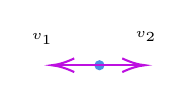
\begin{tikzpicture}[x=0.75pt,y=0.75pt,yscale=-1,xscale=1]
%uncomment if require: \path (0,300); %set diagram left start at 0, and has height of 300

%Shape: Circle [id:dp8577753533756336] 
\draw  [color={rgb, 255:red, 74; green, 144; blue, 226 }  ,draw opacity=1 ][fill={rgb, 255:red, 74; green, 144; blue, 226 }  ,fill opacity=1 ] (196.17,140) .. controls (196.17,138.94) and (197.03,138.09) .. (198.09,138.09) .. controls (199.14,138.09) and (200,138.94) .. (200,140) .. controls (200,141.06) and (199.14,141.91) .. (198.09,141.91) .. controls (197.03,141.91) and (196.17,141.06) .. (196.17,140) -- cycle ;
%Straight Lines [id:da03072071750773664] 
\draw [color={rgb, 255:red, 189; green, 16; blue, 224 }  ,draw opacity=1 ]   (198.09,140) -- (177,140) ;
\draw [shift={(175,140)}, rotate = 360] [color={rgb, 255:red, 189; green, 16; blue, 224 }  ,draw opacity=1 ][line width=0.75]    (10.93,-3.29) .. controls (6.95,-1.4) and (3.31,-0.3) .. (0,0) .. controls (3.31,0.3) and (6.95,1.4) .. (10.93,3.29)   ;
%Straight Lines [id:da26303253715785346] 
\draw [color={rgb, 255:red, 189; green, 16; blue, 224 }  ,draw opacity=1 ]   (198.09,140) -- (218,140) ;
\draw [shift={(220,140)}, rotate = 180] [color={rgb, 255:red, 189; green, 16; blue, 224 }  ,draw opacity=1 ][line width=0.75]    (10.93,-3.29) .. controls (6.95,-1.4) and (3.31,-0.3) .. (0,0) .. controls (3.31,0.3) and (6.95,1.4) .. (10.93,3.29)   ;

% Text Node
\draw (164,123.4) node [anchor=north west][inner sep=0.75pt]  [font=\tiny]  {$v_{1}$};
% Text Node
\draw (214,122.4) node [anchor=north west][inner sep=0.75pt]  [font=\tiny]  {$v_{2}$};


\end{tikzpicture}

\end{center}

首先我们对初速度(这里初速度为$\vec{0}$)进行平行四边形分解,由于初始时速度为$0$,故我们可以分解成两个等大反向的速度(即$v_1$和$v_2$等大反向)。$v_1$和$v_2$在磁场中分别产生洛伦兹力,且\textbf{物体受到的总的洛伦兹力可以表示为$v_1$、$v_2$分别产生的洛伦兹力的矢量合成}。其中,\textbf{我们希望$v_2$产生的洛伦兹力可以抵消重力},故
$$v_2=\frac{mg}{Bq}$$
则$v_2$引起的运动为向右的匀速直线运动。由于$v_1$和$v_2$等大反向,故$v_1 = v_2$(只考虑大小,不考虑方向)。由于$v_2$产生的洛伦兹力抵消了重力,那么分析$v_1$造成的运动时可不考虑重力,故$v_1$会使得物体做圆周运动,其半径为
$$R = \frac{m v_1}{B q} = \frac{m^2 g}{B^2 q^2}$$
\textbf{物体实际的运动为$v_2$引起的向右匀速直线运动和$v_1$引起的逆时针圆周运动的合成},实际轨迹见下图(取$R=1$,$v_1=v_2=1$)

\begin{figure}[htbp]
\centering
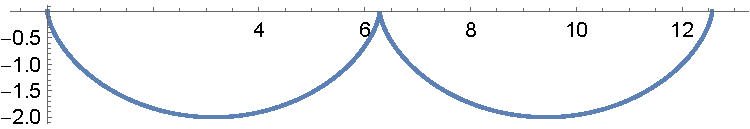
\includegraphics[width=0.5\textwidth]{pic_eled/psf_p3.pdf}
\end{figure}

\subsection{电磁场换系角度介绍“配速法”}

借助前文\secref{s_dcchx},我们可以从另一个角度分析配速法。考虑同样的情景,如图,一个带点小球位于坐标原点,其质量为$m$,电荷量为$q$,位于磁场强度为$B$的水平磁场中,初速度为$0$,试分析其运动。

\begin{center}



\tikzset{every picture/.style={line width=0.75pt}} %set default line width to 0.75pt        

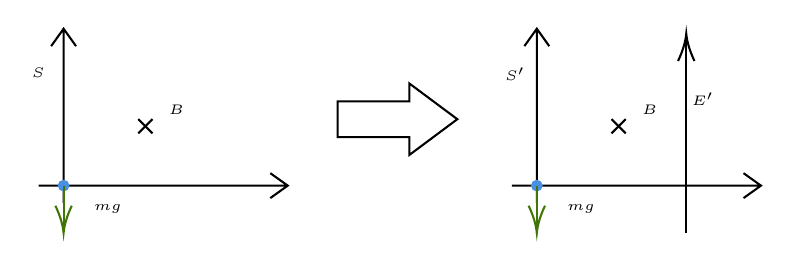
\begin{tikzpicture}[x=0.75pt,y=0.75pt,yscale=-1.2,xscale=1.2]
%uncomment if require: \path (0,300); %set diagram left start at 0, and has height of 300

%Straight Lines [id:da869864321489574] 
\draw    (210,94.3) -- (215.7,100) ;
%Straight Lines [id:da7393063880787207] 
\draw    (215.7,94.3) -- (210,100) ;

%Shape: Axis 2D [id:dp2610193597490549] 
\draw  (170,121) -- (270,121)(180,58) -- (180,128) (263,116) -- (270,121) -- (263,126) (175,65) -- (180,58) -- (185,65)  ;
%Shape: Circle [id:dp711598281784179] 
\draw  [color={rgb, 255:red, 74; green, 144; blue, 226 }  ,draw opacity=1 ][fill={rgb, 255:red, 74; green, 144; blue, 226 }  ,fill opacity=1 ] (178.09,121) .. controls (178.09,119.94) and (178.94,119.09) .. (180,119.09) .. controls (181.06,119.09) and (181.91,119.94) .. (181.91,121) .. controls (181.91,122.06) and (181.06,122.91) .. (180,122.91) .. controls (178.94,122.91) and (178.09,122.06) .. (178.09,121) -- cycle ;
%Straight Lines [id:da05120481576189717] 
\draw [color={rgb, 255:red, 65; green, 117; blue, 5 }  ,draw opacity=1 ]   (180,121) -- (180,138) ;
\draw [shift={(180,140)}, rotate = 270] [color={rgb, 255:red, 65; green, 117; blue, 5 }  ,draw opacity=1 ][line width=0.75]    (10.93,-3.29) .. controls (6.95,-1.4) and (3.31,-0.3) .. (0,0) .. controls (3.31,0.3) and (6.95,1.4) .. (10.93,3.29)   ;
%Straight Lines [id:da6674644989552678] 
\draw    (400,94.3) -- (405.7,100) ;
%Straight Lines [id:da20624873275002797] 
\draw    (405.7,94.3) -- (400,100) ;

%Shape: Axis 2D [id:dp8282527076559207] 
\draw  (360,121) -- (460,121)(370,58) -- (370,128) (453,116) -- (460,121) -- (453,126) (365,65) -- (370,58) -- (375,65)  ;
%Shape: Circle [id:dp6046113343970185] 
\draw  [color={rgb, 255:red, 74; green, 144; blue, 226 }  ,draw opacity=1 ][fill={rgb, 255:red, 74; green, 144; blue, 226 }  ,fill opacity=1 ] (368.09,121) .. controls (368.09,119.94) and (368.94,119.09) .. (370,119.09) .. controls (371.06,119.09) and (371.91,119.94) .. (371.91,121) .. controls (371.91,122.06) and (371.06,122.91) .. (370,122.91) .. controls (368.94,122.91) and (368.09,122.06) .. (368.09,121) -- cycle ;
%Straight Lines [id:da7526857324404845] 
\draw [color={rgb, 255:red, 65; green, 117; blue, 5 }  ,draw opacity=1 ]   (370,121) -- (370,138) ;
\draw [shift={(370,140)}, rotate = 270] [color={rgb, 255:red, 65; green, 117; blue, 5 }  ,draw opacity=1 ][line width=0.75]    (10.93,-3.29) .. controls (6.95,-1.4) and (3.31,-0.3) .. (0,0) .. controls (3.31,0.3) and (6.95,1.4) .. (10.93,3.29)   ;
%Right Arrow [id:dp6817029209016499] 
\draw   (290,87.17) -- (318.85,87.17) -- (318.85,80) -- (338.09,94.33) -- (318.85,108.67) -- (318.85,101.5) -- (290,101.5) -- cycle ;
%Straight Lines [id:da6241127557743624] 
\draw    (430,140) -- (430,62) ;
\draw [shift={(430,60)}, rotate = 90] [color={rgb, 255:red, 0; green, 0; blue, 0 }  ][line width=0.75]    (10.93,-3.29) .. controls (6.95,-1.4) and (3.31,-0.3) .. (0,0) .. controls (3.31,0.3) and (6.95,1.4) .. (10.93,3.29)   ;

% Text Node
\draw (221,87.4) node [anchor=north west][inner sep=0.75pt]  [font=\tiny]  {$B$};
% Text Node
\draw (191,127.4) node [anchor=north west][inner sep=0.75pt]  [font=\tiny]  {$mg$};
% Text Node
\draw (166,72.4) node [anchor=north west][inner sep=0.75pt]  [font=\tiny]  {$S$};
% Text Node
\draw (411,87.4) node [anchor=north west][inner sep=0.75pt]  [font=\tiny]  {$B$};
% Text Node
\draw (381,127.4) node [anchor=north west][inner sep=0.75pt]  [font=\tiny]  {$mg$};
% Text Node
\draw (356,72.4) node [anchor=north west][inner sep=0.75pt]  [font=\tiny]  {$S^{\prime }$};
% Text Node
\draw (431,82.4) node [anchor=north west][inner sep=0.75pt]  [font=\tiny]  {$E^{\prime }$};


\end{tikzpicture}


\end{center}

如图,我们记相对地面静止的参考系为$S$系,\textbf{由于$S$系中物体受到重力和磁场力,运动较难分析,故我们考虑选取一个新的参考系$S^{\prime}$,使得在$S^{\prime}$中存在一个方向向上的电场$E^{\prime}$,与重力$mg$抵消,使得在$S^{\prime}$系中物体做匀速圆周运动}。(见\secref{s_dcchx})

在$S^{\prime}$系中,由于电场力与重力抵消,故$E^{\prime} q = m g$。根据\theoref{d_dcchx},有$E^{\prime} = B v$,故$S^{\prime}$系相对$S$系以速度$v = \frac{mg}{Bq}$向右运动。

由于$S^{\prime}$系相对$S$系以速度$v$向右运动,初始时物体相对$S$系速度为$0$,根据\secref{s_sdql},在$S^{\prime}$系中,初始时物体速度$v^{\prime} = 0 - v = -\frac{mg}{Bq}$,负号代表方向向左。根据前文物体在$S^{\prime}$系中做匀速圆周运动,故圆周运动半径为(计算时忽略了$v^{\prime}$的负号,只考虑大小)

$$R = \frac{mv^{\prime}}{Bq} = \frac{m^2 g}{B^2 q}$$

根据\secref{s_sdql},物体在$S$系中的运动为物体在$S^{\prime}$系的运动与$S^{\prime}$系相对$S$系运动的叠加,故\textbf{物体实际的运动为$S^{\prime}$系相对$S$系运动引起的以速度$v$向右匀速直线运动和在$S^{\prime}$系运动引起的半径为$R$的逆时针圆周运动的合成}。

\subsection{配速法与粒子汇聚}

\begin{mk}{注意}{}
这里所讲与一般所讲的圆形磁场的“磁汇聚”并不相同,此模型笔者在写此章节时没有在任何参考书中见过,考的可能性也不大,但由于较有意思,故在此介绍。
\end{mk}

\begin{center}

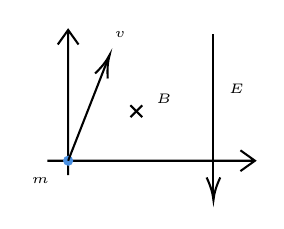
\begin{tikzpicture}[x=0.75pt,y=0.75pt,yscale=-1,xscale=1]
%uncomment if require: \path (0,300); %set diagram left start at 0, and has height of 300

%Straight Lines [id:da869864321489574] 
\draw    (210,94.3) -- (215.7,100) ;
%Straight Lines [id:da7393063880787207] 
\draw    (215.7,94.3) -- (210,100) ;

%Shape: Axis 2D [id:dp2610193597490549] 
\draw  (170,121) -- (270,121)(180,58) -- (180,128) (263,116) -- (270,121) -- (263,126) (175,65) -- (180,58) -- (185,65)  ;
%Shape: Circle [id:dp711598281784179] 
\draw  [color={rgb, 255:red, 74; green, 144; blue, 226 }  ,draw opacity=1 ][fill={rgb, 255:red, 74; green, 144; blue, 226 }  ,fill opacity=1 ] (178.09,121) .. controls (178.09,119.94) and (178.94,119.09) .. (180,119.09) .. controls (181.06,119.09) and (181.91,119.94) .. (181.91,121) .. controls (181.91,122.06) and (181.06,122.91) .. (180,122.91) .. controls (178.94,122.91) and (178.09,122.06) .. (178.09,121) -- cycle ;
%Straight Lines [id:da6241127557743624] 
\draw    (250,60) -- (250,138) ;
\draw [shift={(250,140)}, rotate = 270] [color={rgb, 255:red, 0; green, 0; blue, 0 }  ][line width=0.75]    (10.93,-3.29) .. controls (6.95,-1.4) and (3.31,-0.3) .. (0,0) .. controls (3.31,0.3) and (6.95,1.4) .. (10.93,3.29)   ;
%Straight Lines [id:da5680319150859066] 
\draw    (180,121) -- (199.27,71.86) ;
\draw [shift={(200,70)}, rotate = 111.41] [color={rgb, 255:red, 0; green, 0; blue, 0 }  ][line width=0.75]    (10.93,-3.29) .. controls (6.95,-1.4) and (3.31,-0.3) .. (0,0) .. controls (3.31,0.3) and (6.95,1.4) .. (10.93,3.29)   ;

% Text Node
\draw (221,87.4) node [anchor=north west][inner sep=0.75pt]  [font=\tiny]  {$B$};
% Text Node
\draw (161,127.4) node [anchor=north west][inner sep=0.75pt]  [font=\tiny]  {$m$};
% Text Node
\draw (256,82.4) node [anchor=north west][inner sep=0.75pt]  [font=\tiny]  {$E$};
% Text Node
\draw (201,57.4) node [anchor=north west][inner sep=0.75pt]  [font=\tiny]  {$v$};


\end{tikzpicture}

\end{center}

如图所示,在如图所示复合场中,原点处有一个粒子源,向外发射质量为$m$,带电量为$q$的粒子,初速度为$v$,方向任意。根据前文“配速法”,我们可知任意粒子运动为向右匀速直线运动$v^{\prime}$跟匀速圆周运动叠加而成。由前文易知,向右匀速直线运动$v^{\prime}$满足(注意,前面除磁场外的力为重力,这里为电场力)

$$v^{\prime} = \frac{E}{B}$$

由于磁场中匀速圆周运动周期$T = \frac{2 \pi m}{Bq}$与速度无关,故\textbf{无论粒子初速度大小和方向,其分运动中的匀速圆周运动周期$T$相同,在$n T$的时间后回到原处}($n \in \mathbb{N^{+}}$)\footnote{$\mathbb{N^{+}}$为非零实数集},此时,分运动中的匀速向右运动经过的路程为

$$x = v^{\prime} \cdot n T = n \cdot \frac{2 \pi m E}{B^2 q}$$

可以看到此路程与粒子初速度大小和方向无关,因此,\textbf{在经过$nT$的时间后,粒子分运动中匀速向右运动距离相同,圆周运动均回到原处,故粒子会汇聚在$n \cdot \frac{2 \pi m E}{B^2 q}$处,与粒子初速度大小和方向无关。}

\section{通用“左手定则” \quad * \protect \footnote{带“*”号为娱乐章节,仅介绍一下笔者一些自认为有意思的想法,可选择不读}}

\label{s_tyzsdz}

\begin{mk}{警告}{}
此章节为娱乐章节,仅介绍一下笔者一些自认为有意思的想法,\textbf{如读者感到疑惑或者已有自己习惯,用不习惯此方法,大可将此章节直接抛掉}。
\end{mk}

在高中阶段,我们有描述安培力和洛伦兹力方向的“左手定则”,也有描述动生电动势方向的“右手定则”。有时我们会搞混“左手定则”和“右手定则”,造成方向的误判。故笔者提出一种新的通用的“左手定则”,均使用左手来判断上述三种情况的方向。相比原本的两个定则,笔者认为这个新的方法更不容易出错,并且在做题中更方便。

首先,我们要引入叉乘的概念

\begin{defi}[label=d_cc]{叉乘}{}
叉乘\footnote{又称为外积、向量积、叉积}是两个向量之间的运算,两个向量的叉乘得到的还是向量,向量$\vec{a}$与向量$\vec{b}$的叉乘记为$\vec{a} \times \vec{b}$
~\\

\textbf{叉乘的模}  \quad 两向量叉乘得到的向量的模长满足

$$ | \vec{a} \times \vec{b} | = | \vec{a} | | \vec{b} | \sin \theta$$

其中$\theta$为向量$\vec{a}$与向量$\vec{b}$的夹角,可以看到对于叉乘的模长与我们所熟悉的点乘相比只需要将点乘的$\cos \theta$替换为$\sin \theta$即可\footnote{此时你可以注意到叉乘模长的运算形式与安培力、洛伦兹力、动生电动势的式子形式相似}。
~\\

\textbf{叉乘的方向} \quad 记$\vec{c} = \vec{a} \times \vec{b}$,则$\vec{c}$与$\vec{a}$和$\vec{b}$所在平面垂直,且满足“右手定则”,即伸开右手,使得拇指与其余四个手指垂直,且与手掌在同一平面内,让四指先指向第一个向量($\vec{a}$),后弯向第二个向量($\vec{b}$),此时拇指所在方向即为叉乘方向($\vec{c}$)。
~\\

\textbf{叉乘的反交换律} \quad 叉乘有如下所示的重要性质,可通过右手定则验证

$$\vec{a} \times \vec{b} = - \vec{b} \times \vec{a}$$

\end{defi}

\begin{figure}[htbp]
\centering
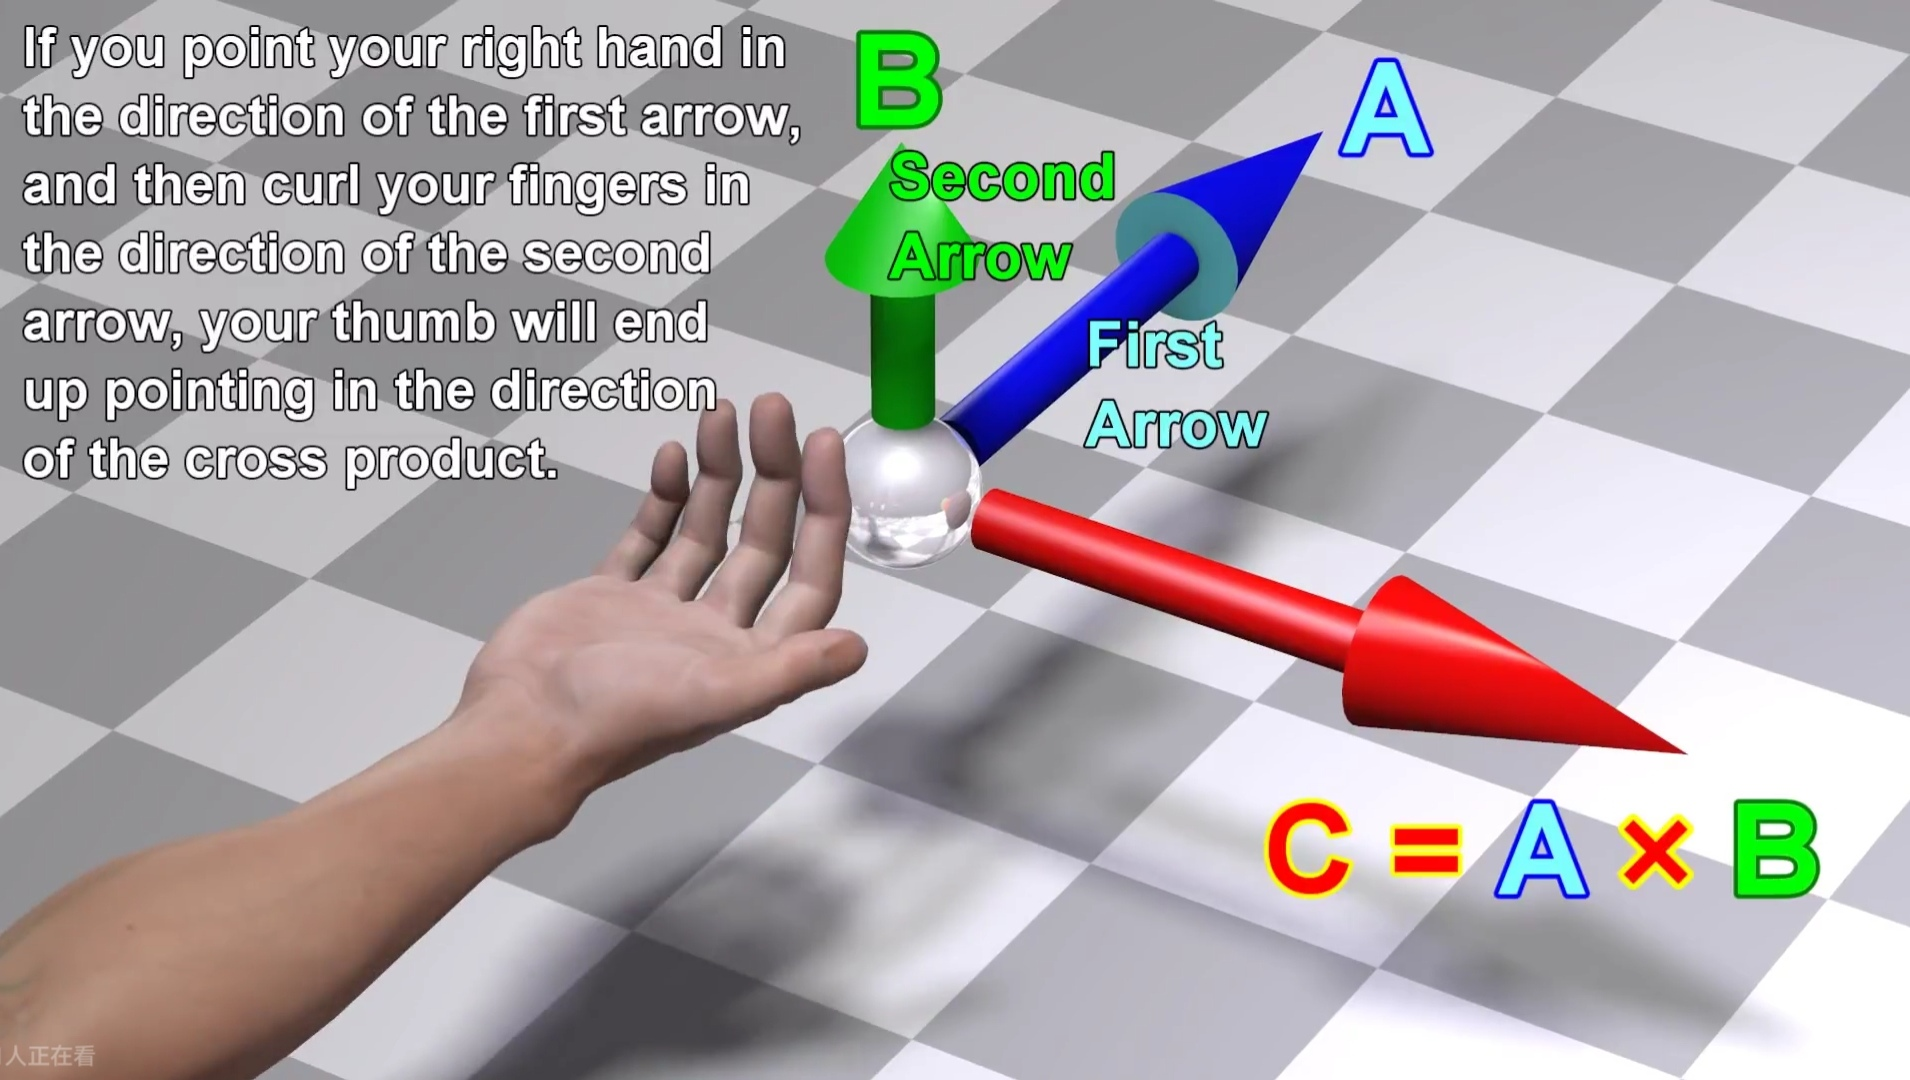
\includegraphics[width=0.6\textwidth]{pic_eled/xxsyt.jpg}
\caption{右手定制判断叉乘方向\protect \footnotemark[\value{footnote}]}
\end{figure}

\footnotetext[\value{footnote}]{截图自视频\url{https://b23.tv/gvNiqfm}}

对于安培力、洛伦兹力、动生电动势,其矢量式分别为

$$\vec{F} = I \vec{L} \times \vec{B}, \quad \vec{F} = q \vec{v} \times \vec{B}, \quad \ms E = (\vec{v} \times \vec{B}) \cdot \vec{L}$$

上式中$\vec{L}$的方向定义为导线中电流的方向。对于第三个式子,若只考虑$\vec{v} \times \vec{B}$与$\vec{L}$平行的情况(高中中绝大多数都是这种情况),结合前文提到的叉乘的反交换律,则上面三式可改写为

$$\vec{F} = - I \vec{B} \times \vec{L}, \quad \vec{F} = - q \vec{B} \times \vec{v}, \quad \ms E = L | (- \vec{B}) \times \vec{v} |$$

从上面三式可以看出,其都为$\vec{B}$叉乘其他矢量的结构(提出负号),且被叉乘的矢量为“原因”,得到的量为“结果”。而前面的负号可以通过将“右手定则”改为“左手定则”而自动加上。因此,我们可以得到如下的新“左手定则”

\begin{theo}{通用“左手定则”}{}
类似前文提到的“右手定则”,伸开\textbf{左手},使得拇指与其余四个手指垂直,且与手掌在同一平面内,\textbf{让四指先指向磁场方向,后弯向“因”,此时拇指所在方向即为“果”}。

这里需要对上面的“原因”和“结果”进一步说明:

\begin{itemize}
	\item \textbf{安培力} \quad 因为有电流,故产生了安培力。电流为“因”,安培力为“果”
	\item \textbf{洛伦兹力} \quad 因为有速度,产生了电流\footnote{正电荷电流方向跟运动方向相同,负电荷相反},故产生了洛伦兹力。电流为“因”,洛伦兹力为“果”
	\item \textbf{动生电动势} \quad 因为有速度,故产生了电流\footnote{这里电流为电源内部电流,故电流流向电源正极,即拇指方向指向电源正极}。速度为“因”,电动势为“果”
\end{itemize}

\end{theo}

可见,运用此方法,我们可以将安培力、洛伦兹力、动生电动势方向均可以使用通用“左手定则”判断。且还有一个好处,运用此方法,我们不需要想象磁场线在垂直手掌方向的分量,磁场与“因”的方向可以不是$90^{\circ}$,而是任意度数(只有弯手掌时不弯$90^{\circ}$即可)